\documentclass[a4paper,12pt]{article}
\usepackage{fontspec}
\usepackage{xeCJK}
\setmainfont{Times New Roman}
\usepackage{amsmath}
\usepackage{amsthm}
\usepackage{amsfonts}
\usepackage{amssymb}
\usepackage{graphicx}
\usepackage{hyperref}
\usepackage{enumitem}
\usepackage{textcomp}
\usepackage{float}
\usepackage{booktabs}
\usepackage{url}
\usepackage[colorinlistoftodos]{todonotes}
\usepackage[left=1.50cm, right=1.50cm, top=1.20cm]{geometry}
\linespread{1.5}
\usepackage{algorithm}
\usepackage{algpseudocode}
\usepackage{tikz}
\usetikzlibrary{matrix, positioning, fit, calc, arrows, intersections, shapes, decorations.markings}
\usepackage{upquote}
\usepackage{listings}
\usepackage{color}
\usepackage{subcaption}
\usepackage[tikz]{mdframed}
\lstdefinestyle{customc}{
  belowcaptionskip=1\baselineskip,
  breaklines=true,
  frame=L,
  xleftmargin=\parindent,
  language=C++,
  tabsize=2,
  %numbers=left,
  %stepnumber=1,
  showstringspaces=false,
  basicstyle=\small\ttfamily,
  keywordstyle=\bfseries\color{green!40!black},
  commentstyle=\itshape\color{purple!40!black},
  identifierstyle=\color{blue},
  stringstyle=\color{orange},
}
\mdfdefinestyle{mymdf}{leftmargin=1cm,rightmargin=2cm,%
innerleftmargin=1cm,innerrightmargin=1cm,roundcorner=10pt,backgroundcolor=lg}
\definecolor{lg}{RGB}{247,249,250}
\title{Algorithm Problem Set \\ \large No. 300 --- 399}
\author{SS}

\begin{document}
\renewcommand{\thelstlisting}{\thesection.\arabic{lstlisting}}
\newcommand{\fcc}[1]{\lstinline[language=C++, basicstyle=\small\ttfamily, keywordstyle=\bfseries\color{green!40!black}]|#1|}
\newcommand{\fcj}[1]{\lstinline[language=Java, basicstyle=\small\ttfamily, keywordstyle=\bfseries\color{green!40!black}]|#1|}
%\sloppy
\maketitle
\section{300. Longest Increasing Subsequence}
Given an unsorted array of integers $A$, find the length of longest increasing subsequence.

\paragraph{Example:}

\begin{flushleft}
\textbf{Input}: [10, 9, 2, 5, 3, 7, 101, 18]
\\
\textbf{Output}: 4 
\\
\textbf{Explanation}: The longest increasing subsequence is [2, 3, 7, 101], therefore the length is 4.
\end{flushleft} 

\paragraph{Note:}
\begin{itemize}
\item There may be more than one LIS combination, it is only necessary for you to return the length.
\item Your algorithm should run in $O(n^2)$ complexity.
\end{itemize}

\paragraph{Follow up:} 
\begin{itemize}
\item Could you improve it to $O(n \log n)$ time complexity?
\end{itemize}

\subsection{Dynamic Programming}
\begin{itemize}
\item 这是典型的循环式DP。
\item Suppose $F[i]$表示以 $A[i]$为结尾的LIS的长度,
\item 对于每一个$A[i]$,从$A[0]$循环到$A[i-1]$,如果发现其中某个数$A[j] < A[i]$, update $F[i]$ as $F[i]\gets \max(F[i], F[j] + 1)$。
\item 在上述update $F[i]$时,同时记录current maximum $F[i]$ as $\ell$。
\item At the end,$\ell$就是global LIS的长度。
\end{itemize}

\setcounter{algorithm}{0}
\begin{algorithm}[H]
\caption{Dynamic Programming}
\begin{algorithmic}[1]
\Procedure{LengthOfLIS}{$A, L$}
\State $\star$ create an array $F$ with size $L$ as DP array
\State $\star$ Set all elements in $F$ as 1
\State $\star$ Set result LIS $\ell$ as 1
\For{$i:=1$ \textbf{to} $L-1$}
\For{$j:=0$ \textbf{to} $i-1$}
\algstore{300algo}
\end{algorithmic}
\end{algorithm}
\begin{algorithm}[H]
\begin{algorithmic}[1]
\algrestore{300algo}
\If{$A[j] < A[i]$}
\State $F[i]\gets \max(F[i], F[j]+1)$
\State $\ell\gets\max(\ell, F[i])$
\EndIf
\EndFor
\EndFor
\State \Return $\ell$
\EndProcedure
\end{algorithmic}
\end{algorithm}

\setcounter{lstlisting}{0}
\begin{lstlisting}[style=customc, caption={Dynamic Programming}]
int lengthOfLIS( vector<int>& nums )
{
    if( nums.empty() )
    {
        return 0;
    }

    vector<int> F( nums.size(), 1 );

    int ans = 1;

    for( size_t i = 1; i < nums.size(); ++i )
    {
        for( size_t j = 0; j < i; ++j )
        {
            if( nums[j] < nums[i] )
            {
                F[i] = ( max )( F[i], F[j] + 1 );
                //update global maximum LIS
                ans = ( max )( ans, F[i] );
            }
        }
    }

    return ans;
}
\end{lstlisting}

\subsection{Binary Search}
\begin{enumerate}
\item 初始化一个array $F$,最初为empty。
\item 遍历输入数组$A$,对于每个$A[i]$,用leftmost binary search在$F$中查找第一个不小于$A[i]$的值 $F[\omega]$,
\item 如果这个值不存在,就把$A[i]$加入到$F$
\item 否则,将$F[\omega]$替换为$A[i]$。
\item 最后返回$F$的size。
\item 特别注意的是$F$可能不是一个真实的LIS,只是长度和LIS相等。
\end{enumerate}

\begin{algorithm}[H]
\caption{Binary Search}
\begin{algorithmic}[1]
\Procedure{LengthOfLIS}{$A, L$}
\State $\star$ Create an empty array $F$
\State $\star$ Add $A[0]$ to $F$
\For{$i:=1$ \textbf{to} $L-1$}
\State $\star$ leftmost binary search $F$ to find the first index $\omega$ where $F[\omega]\geq A[i]$
\If{$\omega=\lvert F\vert$} \Comment $A[i]$ is largest for all elements in $F$
\State  $\star$ Add $A[i]$ to $F$
\Else
\State $F[\omega]\gets A[i]$ \Comment Update $F[\omega]$ to $A[i]$
\EndIf
\EndFor
\State \Return $ \lvert F\vert $ \Comment Return the size of $F$
\EndProcedure
\end{algorithmic}
\end{algorithm}

\begin{lstlisting}[style=customc, caption={Binary Search}]
int lengthOfLIS( vector<int>& nums )
{

    if( nums.empty() )
    {
        return 0;
    }

    vector<int> F;
    F.reserve( nums.size() );

    F.push_back( nums[0] );

    for( size_t i = 1; i < nums.size(); ++i )
    {

        auto p = leftmost( F, nums[i] );

        if( p == F.size() )
        {
            //no any number in F is no less than nums[i]
            F.push_back( nums[i] );
        }
        else
        {
            //update F[p] as nums[i]
            F[p] = nums[i];
        }
    }

    //The size of F is the length
    //but F itself maynot be LIS
    return F.size();
}

//leftmost binary search
size_t leftmost( vector<int>& A, int x )
{
    size_t l = 0;
    size_t r = A.size();

    while( l < r )
    {
        auto mid = ( l + r ) / 2;
        if( A[mid] < x )
        {
            l = mid + 1;
        }
        else
        {
            r = mid;
        }
    }

    return l;
}
\end{lstlisting}

\paragraph{Related Problems}
\begin{itemize}
\item \textbf{334. Increasing Triplet Subsequence}
\item \textbf{354. Russian Doll Envelopes}
\item \textbf{646. Maximum Length of Pair Chain}
\item \textbf{673. Number of Longest Increasing Subsequence}
\end{itemize}
% \section{301 --- Remove Invalid Parentheses}
Remove the minimum number of invalid parentheses in order to make the input string valid. Return all possible results.
\par
\textbf{Note:} The input string may contain letters other than the parentheses ( and ).

\paragraph{Example 1:}

\begin{flushleft}
\textbf{Input}: $()())()$
\\
\textbf{Output}: [$()()()$, $(())()$]
\\
\end{flushleft}

\paragraph{Example 2:}

\begin{flushleft}
\textbf{Input}: $(a)())()$
\\
\textbf{Output}: [$(a)()()$, $(a())()$]
\end{flushleft}

\paragraph{Example 3:}


\begin{flushleft}
\textbf{Input}: )(
\\
\textbf{Output}: []
\end{flushleft}
\subsection{Backtracking}
\begin{itemize}
	\item 对每一个括号,都有两个选择,加入或者不加入最终的expression。
	\item 由于每个选择都要进行测试,因此可以通过递归的方法生成。
	\item 递归的状态由当前$S$中的index $p$来确定,同时递归的状态中加入$x$和$y$分别代表已经加入expression的左括号和右括号的个数。同时,递归的状态中还包括从$S$中不加入expression的字符的counter $z$。
	\item 如果$S[p]$不是左括号或者右括号,直接加入到生成的expresssion。
	\item 如果$S[p]$是左括号或者右括号,那么如上所述,可以把$S[p]$加入或者不加入到expression中。
	\begin{enumerate}
		\item 首先选择不加入,然后继续递归,这时候$x$和$y$都不变,但是记录不加入expression的字符个数的counter $z$ increments。
		\item 然后选择加入。
		\begin{itemize}
			\item 如果$S[p]$是左括号,$x$ increments,其余状态都不变
			\item 如果$S[p]$是右括号,这时候要判断$y$和$x$的关系,如果$y>x$,即右括号个数大于左括号个数,这时候就不用继续递归了,因为这时候一定不是valid expression。否则,继续递归,$y$ increments,其余状态不变。
		\end{itemize}
	\end{enumerate}
\item 当$p$equal to $S$的length时,如果$x$和$y$相等,表示expression是valid string。但这时候需要比较$z$是否比之前获得的最少的count of characters removed,如果相等,加入最终的结果中,如果$z$还要小,那么$z$最新的global minimum count,这时候要把结果清空,然后加入当前的expression。
\item 为了避免重复的string,用一个hash set来存放expression。
\end{itemize}
\begin{algorithm}[H]
	\caption{Recursion}
	\begin{algorithmic}[1]
		\Procedure{RemoveInvalidParentheses}{$S, L$}
		\State $\star$ Create an empty hash set $A$ to store the valid expressions
		\State $\star$ Create an empty string $E$ to store current valid expression
		\State $z_0:=0$ \Comment Global minimum count of characters removed from $S$
		\State \Call{DFS}{$S, L, p = 0, x = 0, y = 0, E, A, 0, \hat{z}=z_0$}
		\EndProcedure
	\end{algorithmic}
\end{algorithm}
Function \texttt{DFS}递归生成所有valid parentheses expressions。递归的状态包括
\begin{itemize}
	\item $p$ --- Current index in $S$
	\item $x$, $y$ --- The count of left parentheses and right parentheses
	\item $E$ --- 当前生成的valid expression
	\item $A$ --- 保存所有生成的具有最小count of removed characters的valid expression的hash set
\end{itemize}
\begin{algorithm}[H]
	\caption{Recursion Helper Function}
	\begin{algorithmic}[1]
		\Function{DFS}{$S,L,p,x,y,E,A,z,\hat{z}$}
		\State $\ast$ 递归结束的处理
		\If{$p=L$}
		\If{$x=y$} \Comment 只有当前左括号个数与右括号个数相等时,才是合法的expression
		\If{$z = \hat{z}$} \Comment Removed character个数与当前的global
		 minimum相等
		\algstore{301algo}
		\end{algorithmic}
	\end{algorithm}
\begin{algorithm}[H]
	\begin{algorithmic}[1]
		\algrestore{301algo}
				 \State $\star$ 把$E$加入$A$中
		\ElsIf{$z<\hat{z}$} \Comment Removed character个数比当前的global minmum还要少
		\State $\star$ Clear $A$ 因为$A$中的所有expression比起$E$来更短
		\State $\hat{z}\gets z$ \Comment Update Global minimum count
		\State $\star$ 把$E$加入$A$中
		\EndIf
		\EndIf
		\State \Return 
		\EndIf
		
				\If{$S[p]$既不是左括号也不是右括号}
		\State $\star$ Add $S[p]$ to $E$
		\State $\ast$ 继续下一层递归
		
				\State \Call{DFS}{$S, L, p+1, x, y, E, A, z, \hat{z}$}
		\State $\star$ 上述递归结束后,把$S[p]$从$E$中移除
		
				\Else
		\State $\ast$ 首先选择不把$S[p]$加入$E$中,然后继续下一层递归
		\State \Call{DFS}{$S, L, p+1, x, y, E, A, z+1, \hat{z}$} \Comment 这时候$z$要increments
		\State $\star$ $S[p]$加入$E$中
		\If{$S[p]$是左括号}
		\State $\ast$ 继续下一层递归,这时候$E$中多了一个左括号,因此$x\gets x+1$
		\State \Call{DFS}{$S, L, p+1, x+1, y, E, A, z, \hat{z}$}
		\ElsIf{$x>y$} \Comment 右括号情况下,只有左括号的个数大于右括号个数才能加入这个右括号
		\State $\ast$ 继续下一层递归,这时候$E$中多了一个右括号,因此$y\gets y+1$
		\State \Call{DFS}{$S, L, p+1, x, y+1, E, A, z, \hat{z}$}
		\EndIf
		\State $\star$ 结束后,把$S[p]$从$E$中移除
		\EndIf
		\EndFunction
	\end{algorithmic}
\end{algorithm}
\setcounter{lstlisting}{0}
\begin{lstlisting}[style=customc, caption={Recursive Method 1}]
vector<string> removeInvalidParentheses( string s )
{

    //record the expressions generated during recursion
    unordered_set<string> A;

    string E;

    E.reserve( s.size() );

    int z0 = INT_MAX;

    DFS( s, 0, 0, 0, E, A, 0, z0 );

    return {A.begin(), A.end()};
}

void DFS( const string& S, size_t p, int x, int y, string& expr, unordered_set<string>& A, int z, int& z0 )
{
    if( p == S.size() )
    {
        if( x == y )
        {
            if( z == z0 )
            {
                //current count of removed characters
                //is equal to the global minimum characters
                A.emplace( expr );
            }
            else if( z < z0 )
            {
                //current count of removed characters
                //is less than the global minimum characters
                A.clear();
                A.emplace( expr );

                z0 = z;
            }
        }

        return;
    }

    if( ( S[p] != '(' ) && ( S[p] != ')' ) )
    {
        //Other letters
        //Just add to the expression
        expr.push_back( S[p] );
        DFS( S, p + 1, x, y, expr, A, z, z0 );
        expr.pop_back();
    }
    else
    {
        //First choosing not to add to the expression
        DFS( S, p + 1, x, y, expr, A, z + 1, z0 );

        //Then choose adding to the expression
        expr.push_back( S[p] );

        if( S[p] == '(' )
        {
            //add left parenthesis
            DFS( S, p + 1, x + 1, y, expr, A, z, z0 );
        }
        else if( y < x )
        {
            //Only add right parenthesis when there are fewer right parenthesis than left parenthesis
            //in the expression
            DFS( S, p + 1, x, y + 1, expr, A, z, z0 );
        }

        expr.pop_back();
    }
}
\end{lstlisting}
\subsection{Optimized Recursion}
\begin{itemize}
\item 上述算法中,可以进行更多的prunning。方法是在上述递归的状态中,加入额外两个状态,即number of left misplaced parentheses and number of misplaced right parenthese removed from $S$ to get a valid expression。分别用$\alpha$和$\beta$表示。
\item 为了能够得到上述的额外两个状态的初始值,需要preprocess $S$。方法如下
\begin{itemize}
\item 从左到右扫描$S$
\item 如果遇到一个左括号,这个括号可能会包含在一个valid expression中,取决于在其右边是否存在匹配的右括号。但是这时候我们并不知道,因此just increments 左括号的counter $\alpha$。
\item 如果遇到一个右括号,如果当前左括号个数$\alpha$为零,显然这个右括号不能被匹配,因此increments misplaced的右括号的counter $\beta$。如果$\alpha$不为零,这个右括号可以被之前的一个左括号匹配,而这时候misplaced left parenthese counter $\alpha$就要decrement。
\end{itemize}
\item 由于$\alpha$和$\beta$告诉我们需要remove多少parenthesis,算法需要进行修改一边利用这两个状态信息。
\begin{enumerate}
\item 当前$p$ equal to $S$的length时, 这时候expression is valid的条件是$\alpha=0$ and $\beta=0$,不再需要判定$x$和$y$是否相等了。
\item 当选择不加入当前的左括号或者右括号时,需要检查$\alpha$或者$\beta$是否为零,如果是零,表示不能再remove了,因此也就不能继续进行递归了。
\end{enumerate}
\end{itemize}
\begin{algorithm}[H]
	\caption{Recursion Method 2: More Efficient}
	\begin{algorithmic}[1]
		\Procedure{RemoveInvalidParentheses}{$S, L$}
		\State $\star$ Create an empty hash set $A$ to store the valid expressions
		\State $\star$ Create an empty string $E$ to store current valid expression
		\State $\ast$ Preprocess $S$ to get number of misplaced left and right parentheses
				\algstore{301algo}
				\end{algorithmic}
			\end{algorithm}
		\begin{algorithm}[H]
			\begin{algorithmic}[1]
				\algrestore{301algo}
		\State $\alpha:=0$ and $\beta:=0$
		\For{Each character $c$ in $S$}
		\If{$c$ is left parenthesis}
		\State $\alpha\gets\alpha+1$
		\ElsIf{$c$ is right parenthesis}
		\If{$\alpha=0$}
		\State $\beta\gets\beta+1$ \Comment 不能再找到匹配的左括号
		\Else
		\State $\alpha\gets\alpha-1$ \Comment 有匹配的左括号,decrements $\alpha$
		\EndIf
		\EndIf
		\EndFor
		\State \Call{DFS}{$S, L, p = 0, x = 0, y = 0, \alpha, \beta, E, A$}
		\EndProcedure
	\end{algorithmic}
\end{algorithm}
Function \texttt{DFS}递归生成所有valid parentheses expressions。递归的状态包括
\begin{itemize}
	\item $p$ --- Current index in $S$
	\item $x$, $y$ --- The count of left parentheses and right parentheses
	\item $\alpha$, $\beta$ --- The misplaced number of left and right parentheses
	\item $E$ --- 当前生成的valid expression
	\item $A$ --- 保存所有生成的具有最小count of removed characters的valid expression的hash set
\end{itemize}
\begin{algorithm}[H]
	\caption{Recursion Helper Function}
	\begin{algorithmic}[1]
		\Function{DFS}{$S,L,p,x,y,E,A,z,\hat{z}$}
		\State $\ast$ 递归结束的处理
		\If{$p=L$}
		\If{$\alpha=0$ \textbf{and} $\beta=0$} \Comment No more misplaced parentheses
		\State $\star$ 把$E$加入$A$中
		\EndIf
		\State \Return
		\EndIf
		\algstore{301algo}
		\end{algorithmic}
	\end{algorithm}
\begin{algorithm}[H]
	\begin{algorithmic}[1]
		\algrestore{301algo}	
				\If{$S[p]$既不是左括号也不是右括号}
		\State $\star$ Add $S[p]$ to $E$
		\State $\ast$ 继续下一层递归
		
				\State \Call{DFS}{$S, L, p+1, x, y, \alpha, \beta, E, A$}
		\State $\star$ 上述递归结束后,把$S[p]$从$E$中移除
		
				\Else
		\State $\ast$ 首先选择不把$S[p]$加入$E$中,然后继续下一层递归
		\If{$S[p]$ is left parenthesis}
		\If{$\alpha > 0$}
		\State $\ast$只有当剩下的misplaced left parenthesis 大于零
		\State $\ast$才可以忽略当前的左括号进入下一层递归
		\State  \Call{DFS}{$S, L, p+1, x, y, \alpha-1, \beta, E, A$}
		\EndIf
		\State $\star$ $S[p]$加入$E$中
		\State $\ast$ 继续下一层递归,这时候$E$中多了一个左括号,因此$x\gets x+1$
		\State \Call{DFS}{$S, L, p+1, x+1, y, \alpha, \beta, E, A$}
		\State $\star$ 结束后,把$S[p]$从$E$中移除
		\Else
				\State $\ast$只有当剩下的misplaced right parenthesis 大于零时,
				\State $\ast$ 才可以忽略当前的右括号进入下一层递归
				\State  \Call{DFS}{$S, L, p+1, x, y, \alpha, \beta-1, E, A$}
				\EndIf
				\If{$x>y$} \Comment 右括号情况下,只有左括号的个数大于右括号个数才能加入这个右括号
					\State $\star$ $S[p]$加入$E$中
					\State $\ast$ 继续下一层递归,这时候$E$中多了一个右括号,因此$y\gets y+1$
					\State \Call{DFS}{$S, L, p+1, x, y+1, \alpha, \beta, E, A$}
					\State $\star$ 结束后,把$S[p]$从$E$中移除
				\EndIf	
		\EndIf
		\EndFunction
	\end{algorithmic}
\end{algorithm}
\begin{lstlisting}[style=customc, caption={Recursive Method 1}]
vector<string> removeInvalidParentheses( string s )
{

    unordered_set<string> s_expr;

    string expr;
    expr.reserve( s.size() );

    int alpha = 0;
    int beta = 0;

    //get misplaced left and right parentheses
    for( auto c : s )
    {
        if( c == '(' )
        {
            ++alpha;
        }
        else if( c == ')' )
        {
            if( alpha == 0 )
            {
                ++beta;
            }
            else
            {
                --alpha;
            }
        }
    }

    dfs( s, 0, 0, 0, alpha, beta, expr, s_expr );

    return {s_expr.begin(), s_expr.end()};
}

void dfs( const string& S, size_t p, int x, int y, int alpha, int beta, string& expr, unordered_set<string>& ss )
{
    if( p == S.size() )
    {
        if( ( alpha == 0 ) && ( beta == 0 ) )
        {
            ss.emplace( expr );
        }

        return;
    }

    if( ( S[p] != '(' ) && ( S[p] != ')' ) )
    {
        //Normal letter
        expr.push_back( S[p] );
        dfs( S, p + 1, x, y, alpha, beta, expr, ss );
        expr.pop_back();
    }
    else
    {
        if( S[p] == '(' )
        {
            if( alpha > 0 )
            {
                //only when remained misplaced left parentheses
                //are larger than zero, go to next recursion
                dfs( S, p + 1, x, y, alpha - 1, beta, expr, ss );
            }

            expr.push_back( S[p] );
            dfs( S, p + 1, x + 1, y, alpha, beta, expr, ss );
            expr.pop_back();
        }
        else
        {
            if( beta > 0 )
            {
                //only when remained misplaced right parentheses
                //are larger than zero, go to next recursion
                dfs( S, p + 1, x, y, alpha, beta - 1, expr, ss );
            }

            if( y < x )
            {
                //only when right parentheses is fewer than
                //left parentheses
                expr.push_back( S[p] );
                dfs( S, p + 1, x, y + 1, alpha, beta, expr, ss );
                expr.pop_back();
            }
        }
    }
}
\end{lstlisting}
\subsection{Recursive Method 3: Most Efficient}
\begin{itemize}
\item 每一次递归中,首先检测到哪个位置会出现右括号多于左括号。如果找到了这个位置,就将多余的第一个右括号移除,然后从这个移除的右括号的下一个位置继续下一层递归。
\item 如果这时候检测到左括号多于右括号,那么需要将多余的第一个左括号移除,然后从这个移除的左括号的下一个位置进行递归。但这个时候需要从右到左扫描找到第一个需要移除的左括号。
\item 为了避免从左到右和从右到左使用不同的代码,可以用一个小技巧,将$S$进行翻转,这样从右到左的扫描,就变为从左到右扫描了。
\item 但是这时候有个问题是之前的左括号和右括号的位置发生了变化,为了仍然能够得到valid expression,再得到去除第一个多余的左括号后,把生成的expression再反转一遍。
\item 为了避免在上述过程中得到duplicate expression,如果不使用hash set,可以在递归状态中包含上一次删除的括号的index。这样下一层递归就从这个index开始。
\item 可以使用一个key检查示当前是从左到右删除多余的右括号,还是在翻转字符中从左到右删除多余的左括号。前者这个key是$()$,而后者这个key则是$)($。这样通过比较这个key,就知道当前是要搜索左括号还是右括号作删除,以及当前是否需要翻转$S$。
\end{itemize}
\begin{lstlisting}[style=customc, caption={Recursive Method 3: Most Efficient}]
class Solution
{
public:
    vector<string> removeInvalidParentheses( string s )
    {

        vector<string> ans;

        dfs( s, ans, 0, 0, "()" );

        return ans;
    }

    //x: Last removed position for key[0]
    //y: Last removed position for key[1]
    void dfs( string S, vector<string>& A, size_t x, size_t y, string key )
    {
        int t = 0;

        //The target is to remove additional key[1]
        for( size_t i = x; i < S.size(); ++i )
        {
            if( S[i] == key[0] )
            {
                ++t;
            }
            else if( S[i] == key[1] )
            {
                --t;
            }

            if( t >= 0 )
            {
                //number of key[0] is larger than key[1]
                continue;
            }

            if( y > i )
            {
                //Have not yet reached the last removed position for key[1]
                //No need to further since before y, parenthesis are balanced
                return;
            }

            if( S[y] == key[1] )
            {
                //S[y] is the first index of key[1] after last removed position of key[1]
                dfs( S.substr( 0, y ) + S.substr( y + 1 ), A, i, y, key );
            }

            for( size_t j = y + 1; j <= i; ++j )
            {
                //We found another equal to key[1] candidate to be removed
                //Notice: In this loop, we are searching for candidates to be removed.
                //If there is a consequtive letters equal to key[1]
                //We only need to remove the first one from left to right
                if( ( S[j] == key[1] ) && ( S[j - 1] != key[1] ) )
                {
                    dfs( S.substr( 0, j ) + S.substr( j + 1 ), A, i, j, key );
                }
            }

            return;
        }

        //candidates equal to key[0]
        //is no less than candidiates equal to key[1]
        //We need to reverse, and
        //1. removing right parthesis when now is finding additional right parenthesis
        //2. add reversed string to output when now is finding additional left parenthesis
        reverse( S.begin(), S.end() );

        if( key[0] == '(' )
        {
            //finished left to right scan
            dfs( S, A, 0, 0, ")(" );
        }
        else
        {
            //finished right to left
            A.emplace_back( S );
        }
    }
};
\end{lstlisting}
% \section{302 -- Smallest Rectangle Enclosing Black Pixels}
An image is represented by a binary matrix $M$ with 0 as a white pixel and 1 as a black pixel. The black pixels are connected, i.e., there is only one black region. Pixels are connected horizontally and vertically. Given the location $(x, y)$ of one of the black pixels, return the area of the smallest (axis-aligned) rectangle that encloses all black pixels.
\par
For example, given the following image:
\begin{flushleft}
\begin{table}[H]
\begin{tabular}{cccc}
0 & 0 & 1 & 0\\
0 & 1 & 1 & 0\\
0 & 1 & 0 & 0
\end{tabular}
\end{table}
and $x = 0$, $y = 2$
\par
Return 6.
\end{flushleft}
\subsection{Depth First Search}
\begin{itemize}
\item DFS 搜索,并在递归中记录black pixel的最大和最小的row和col。
\item 为了避免重复搜索,对已经访问过的black pixel标记为2。
\end{itemize}
\setcounter{lstlisting}{0}
\begin{lstlisting}[style=customc, caption={Depth First Search}]
class Solution
{
public:
    int smallestRectangleArea( vector<vector<int>>& image, int x, int y )
    {
        m = static_cast< int >( image.size() );
        n = static_cast< int >( image[0].size() );
        min_x = m;
        min_y = n;
        max_x = -1;
        max_y = -1;

        dfs( image, x, y );
		
        return ( max_x - min_x  + 1 ) * ( max_y - min_y  + 1 );
    }

    void dfs( vector<vector<int>>& M, int x, int y )
    {
        if( ( x < 0 ) || ( x >= m )
                || ( y < 0 ) || ( y >= n )
                || ( M[x][y] != 1 ) )
        {
            return;
        }

        //mark as visited
        M[x][y] = 2;

        min_x = ( min )( x, min_x );
        min_y = ( min )( y, min_y );

        max_x = ( max )( x, max_x );
        max_y = ( max )( y, max_y );


        dfs( M, x - 1, y );
        dfs( M, x + 1, y );
        dfs( M, x, y - 1 );
        dfs( M, x, y + 1 );
    }

private:

    int min_x;
    int max_x;
    int min_y;
    int max_y;

    int m;
    int n;
};
\end{lstlisting}
\subsection{Binary Search}
\begin{itemize}
\item ,以给定的black pixel的坐标$ (x, y) $为中心,用binary search快速找到整个黑色区域的上下左右的临界点,然后直接算出面积。
\item 以寻找黑色连通区域的top为例,因为是top,那么其范围肯定在$ [0, x] $之间。
\begin{enumerate}
\item 假设top在第$ i $行,显然这一行中至少有一个点是black pixel。而这个black pixel的column的范围就在$[0, n]$之间(其中$n$是输入image的宽)。
\item 在进行binary search时,是对row
进行中点计算,然后column从0开始遍历,直到找到为1的点,或者越界位置。目标是从上到下第一个包含有black pixel的row。
\end{enumerate}
\item 寻找bottom与寻找top类似,不同的是,我们是从上到下寻找第一个没有black pixel的行。因此在binary search时,如果middle row包含有black pixel,要将binary search的左边界更新为middle row$  + 1 $。
\item 对于left和right的寻找,与top和bottom的寻找相类似,只不过寻找的是column。
\item 由于bottom和right都是从上到下和从左到右第一个没有black pixel的行和列,因此计算面积直接是(bottom $-$ top)$\times$(right $ - $ left)。
\end{itemize}
\begin{lstlisting}[style=customc, caption={Binary Search}]
class Solution
{
public:
    int smallestRectangleArea( vector<vector<int>>& image, int x, int y )
    {
        m = static_cast< int >( image.size() );
        n = static_cast< int >( image[0].size() );

        int top = topmost( image, 0, x, true );
        int bottom = bottommost( image, y, m, true );
        int left = topmost( image, 0, y, false );
        int right = bottommost( image, y, m, false );

        return ( bottom - top ) * ( right - left );
    }


    int topmost( vector<vector<int>>& M, int l, int r, bool row_mode )
    {
        //find first row/column that contains black pixel
        while( l < r )
        {
            int mid = ( l + r ) / 2;
            bool has_black = false;

            if( row_mode )
            {
                //Searching row
                for( int i = 0; i < n; ++i )
                {
                    if( M[mid][i] == 1 )
                    {
                        has_black = true;
                        break;
                    }
                }
            }
            else
            {
                //Searching Column
                for( int i = 0; i < m; ++i )
                {
                    if( M[i][mid] == 1 )
                    {
                        has_black = true;
                        break;
                    }
                }
            }

            if( !has_black )
            {
                l = mid + 1;
            }
            else
            {
                r = mid;
            }
        }

        return l;
    }

    int bottommost( vector<vector<int>>& M, int l, int r, bool row_mode )
    {
        //find first row/column that does not contain black pixel
        while( l < r )
        {
            int mid = ( l + r ) / 2;
            bool has_black = false;

            if( row_mode )
            {
                //Search for row
                for( int i = 0; i < n; ++i )
                {
                    if( M[mid][i] == 1 )
                    {
                        has_black = true;
                        break;
                    }
                }
            }
            else
            {
                //Search for column
                for( int i = 0; i < m; ++i )
                {
                    if( M[i][mid] == 1 )
                    {
                        has_black = true;
                        break;
                    }
                }
            }


            if( has_black )
            {
                l = mid + 1;
            }
            else
            {
                r = mid;
            }
        }

        return l;
    }


private:

    int m;
    int n;
};
\end{lstlisting}
% \section{303 --- Range Sum Query - Immutable}

\textbf{Easy}

Given an integer array \fcj{nums}, find the sum of the elements between indices $i$ and $j$ ($i \leq j$), inclusive.

\paragraph{Example:}

\begin{flushleft}
\textbf{Input}:  \fcj{nums = [-2, 0, 3, -5, 2, -1]}

\fcj{sumRange(0, 2) -> 1}

\fcj{sumRange(2, 5) -> -1}

\fcj{sumRange(0, 5) -> -3}
\end{flushleft}

\paragraph{Note:}
\begin{itemize}
\item You may assume that the array does not change.
\item There are many calls to \fcj{sumRange} function.
\end{itemize}

\paragraph{Related Problems}
\begin{itemize}
\item \textbf{304. Range Sum Query 2D - Immutable}
\item \textbf{307. Range Sum Query - Mutable}
\item \textbf{325. Maximum Size Subarray Sum Equals k}
\end{itemize}
% \section{304 --- Range Sum Query 2D - Immutable}
Given a 2D matrix matrix $M$, find the sum of the elements inside the rectangle defined by its upper left corner $(r_1, c_1)$ and lower right corner $(r_2, c_2)$.
\begin{figure}[H]
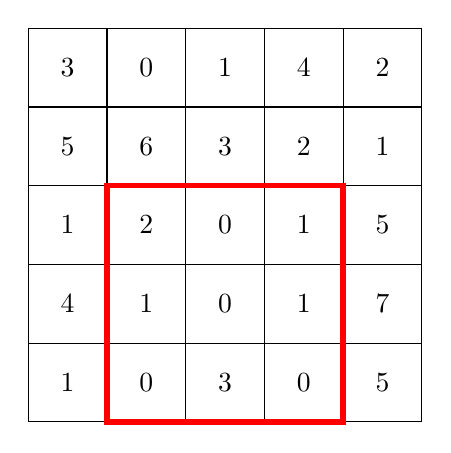
\begin{tikzpicture}
\draw[black, thin] (0,0) grid (5,5);
\node at (0.5,4.5) {$3$};
\node at (1.5,4.5) {$0$};
\node at (2.5,4.5) {$1$};
\node at (3.5,4.5) {$4$};
\node at (4.5,4.5) {$2$};
%row2
\node at (0.5,3.5) {$5$};
\node at (1.5,3.5) {$6$};
\node at (2.5,3.5) {$3$};
\node at (3.5,3.5) {$2$};
\node at (4.5,3.5) {$1$};
%row3
\node at (0.5,2.5) {$1$};
\node at (1.5,2.5) {$2$};
\node at (2.5,2.5) {$0$};
\node at (3.5,2.5) {$1$};
\node at (4.5,2.5) {$5$};
%row 4
\node at (0.5,1.5) {$4$};
\node at (1.5,1.5) {$1$};
\node at (2.5,1.5) {$0$};
\node at (3.5,1.5) {$1$};
\node at (4.5,1.5) {$7$};
%row 5
\node at (0.5,0.5) {$1$};
\node at (1.5,0.5) {$0$};
\node at (2.5,0.5) {$3$};
\node at (3.5,0.5) {$0$};
\node at (4.5,0.5) {$5$};
\draw[line width=2pt,red] (1,0) rectangle ++(3,3);
\end{tikzpicture}
\end{figure}
The above rectangle (with the red border) is defined by $(r_1, c_1) = (2, 1)$ and $(r_2, c_2) = (4, 3)$, which contains sum = 8.
\paragraph{Example:}
\begin{flushleft}
Give matrix $M$ is
\begin{table}[H]
    \begin{tabular}{ccccc}
        3 & 0 & 1 & 4 & 2 \\
        5 &  6 &  3 &  2 &  1\\
        1 &  2 &  0 &  1 &  5 \\
        4 &  1 &  0 &  1 &  7\\
        1 &  0 &  3 &  0 &  5
    \end{tabular}
\end{table}
\begin{lstlisting}[style=customc]
sumRegion(2, 1, 4, 3) // 8
sumRegion(1, 1, 2, 2) // 11
sumRegion(1, 2, 2, 4) // 12
\end{lstlisting}
\end{flushleft}
\paragraph{Note:}
\begin{itemize}
    \item You may assume that the matrix does not change.
    \item There are many calls to \texttt{sumRegion} function.
    \item You may assume that $r_1 \leq r_2$ and $c_1 \leq c_2$.
\end{itemize}
\subsection{Caching}
\begin{itemize}
    \item 这种方法类似于prefix sum的方式,这时候cumulative sum是相对于$(0,0)$的。
\end{itemize}
如下图所示,如果需要计算ABCD部分的sum $S$。将$S$用以$O$为原点的cumulative sum来表示。
\definecolor{lightblue}{RGB}{229,241,255}
\begin{enumerate}
\item Cumulative sum from $O$ to $D$, denote as $S_0$
\begin{figure}[H]
\begin{tikzpicture}
\draw[thin,color=white!60!black!30] (0,0) grid (9,9);
\draw[line width=2pt, color=black] (0,0) rectangle (9,9);
\draw[line width=1pt, color=blue, fill=lightblue, fill opacity=0.3] (0,9) rectangle ++(7,-7);
\node at (0.5,8.5) {$O$};
\node at (3.5,2.5) {$C$};
\node at (3.5,5.5) {$A$};
\node at (6.5,2.5) {$D$};
\node at (6.5,5.5) {$B$};
\draw[line width=2pt, color=red] (3,2) rectangle (7,6);
\end{tikzpicture}
\end{figure}
    \item Cumulative sum from $O$ to the top of $B$, denote as $S_1$
\begin{figure}[H]
\begin{tikzpicture}
\draw[thin,color=white!60!black!30] (0,0) grid (9,9);
\draw[line width=2pt, color=black] (0,0) rectangle (9,9);
\draw[line width=1pt, color=blue, fill=lightblue, fill opacity=0.3] (0,9) rectangle ++(7,-3);
\node at (0.5,8.5) {$O$};
\node at (3.5,2.5) {$C$};
\node at (3.5,5.5) {$A$};
\node at (6.5,2.5) {$D$};
\node at (6.5,5.5) {$B$};
\node at (3.5,7.5) [minimum size=2cm] {\Huge $S_1$};
\draw[line width=2pt, color=red] (3,2) rectangle (7,6);
\end{tikzpicture}
\end{figure}
\item Cumulative sum from $O$ to the left of $C$, denote as $S_2$
\begin{figure}[H]
\begin{tikzpicture}
\draw[thin,color=white!60!black!30] (0,0) grid (9,9);
\draw[line width=2pt, color=black] (0,0) rectangle (9,9);
\draw[line width=1pt, color=blue, fill=lightblue, fill opacity=0.3] (0,9) rectangle ++(3,-7);
\node at (0.5,8.5) {$O$};
\node at (3.5,2.5) {$C$};
\node at (3.5,5.5) {$A$};
\node at (6.5,2.5) {$D$};
\node at (6.5,5.5) {$B$};
\node at (1.5,5.5) [minimum size=2cm] {\Huge $S_2$};
\draw[line width=2pt, color=red] (3,2) rectangle (7,6);
\end{tikzpicture}
\end{figure}
\item Cumulative sum from $O$ to top left of $A$, denote as $S_3$
\begin{figure}[H]
\begin{tikzpicture}
\draw[thin,color=white!60!black!30] (0,0) grid (9,9);
\draw[line width=2pt, color=black] (0,0) rectangle (9,9);
\draw[line width=1pt, color=blue, fill=lightblue, fill opacity=0.3] (0,9) rectangle ++(3,-3);
\node at (0.5,8.5) {$O$};
\node at (3.5,2.5) {$C$};
\node at (3.5,5.5) {$A$};
\node at (6.5,2.5) {$D$};
\node at (6.5,5.5) {$B$};
\node at (1.5,7.5) [minimum size=2cm] {\Huge $S_3$};
\draw[line width=2pt, color=red] (3,2) rectangle (7,6);
\end{tikzpicture}
\end{figure}
\item 注意到$S_1$和$S_2$都包括了$S_3$,因此$S=S_0-S_1-S_2+S_3$
\item 用一个二维数组$F$来记录从$O$到当前坐标$(r,c)$的cumulative sum,注意到$F$的dimension类似于一维的prefix sum,如果matrix的dimension是$m\times n$,那么F的dimension就是$(m+1)\times(n+1)$。因此在坐标$(r,c)$的$F$其实是$F[r+1][c+1]$。于是有$F[r+1][c+1]=F[r+1][c]+F[r][c+1]+M[r][c]-F[r][c]$。因为都$F[r+1][c]$和$F[r][c+1]$都
包括了$F[r][c]$。
\item 对于从$(r_1,c_1)$到$(r_2,c_2)$的sum $S$,用$F$来表示,即为$S=F[r_2+1][c_2+1] - F[r_1][c_2+1] - F[r_2+1][c_1] + F[r_1][c_1]$。其中$F[r_2+1][c_2+1]$, $F[r_1][c_2+1]$,$F[r_2+1][c_1]$和$F[r_1][c_1]$分别为上述分析中的$S_0$,$S_1$,$S_2$和$S_3$
\end{enumerate}
\setcounter{lstlisting}{0}
\begin{lstlisting}[style=customc, caption={Caching}]
class NumMatrix {
public:
    NumMatrix(vector<vector<int>> matrix) {
        
        if(matrix.empty() || matrix[0].empty())
        {
            s=matrix;
            return;
        }
        
        vector<vector<int>> tmp(matrix.size()+1, vector<int>(matrix[0].size()+1,0));
        s.swap(tmp);
        
        for(size_t i = 0; i< matrix.size(); ++i)
        {
            for(size_t j = 0; j < matrix[0].size(); ++j)
            {
                s[i+1][j+1] = s[i+1][j] + s[i][j+1] + matrix[i][j] - s[i][j];
            }
        }
    }
    
    int sumRegion(int row1, int col1, int row2, int col2) {
        if(s.empty() || s[0].empty())
        {
            return 0;
        }
        
        return s[row2+1][col2+1] - s[row1][col2+1] - s[row2+1][col1] + s[row1][col1];
    }
    
    vector<vector<int>> s;
};
\end{lstlisting}
% 
\section{305 --- Number of Islands II}

\textbf{Hard}

A 2d grid map of $m$ rows and $n$ columns is initially filled with water. We may perform an \fcj{addLand} operation which turns the water at position \fcj{(row, col)} into a land. Given a list of positions to operate, count the number of islands after each \fcj{addLand} operation. An island is surrounded by water and is formed by connecting adjacent lands horizontally or vertically. You may assume all four edges of the grid are all surrounded by water.

\paragraph{Example:}

\begin{flushleft}
\textbf{Input}: $m = 3$, $n = 3$, \fcj{positions = [[0,0], [0,1], [1,2], [2,1]]}

\textbf{Output}: \fcj{[1,1,2,3]}

\textbf{Explanation}:

Initially, the 2d grid grid is filled with water. (Assume 0 represents water and 1 represents land).

\[
\begin{bmatrix}
0 & 0 & 0\\
0 & 0 & 0\\
0 & 0 & 0
\end{bmatrix}
\]


Operation 1: \fcj{addLand(0, 0)} turns the water at \fcj{grid[0][0]} into a land.

\[
\begin{bmatrix}
1 & 0 & 0\\
0 & 0 & 0\\
0 & 0 & 0
\end{bmatrix}
\]

Number of islands:  1

Operation 2: \fcj{addLand(0, 1)} turns the water at \fcj{grid[0][1]} into a land.

\[
\begin{bmatrix}
1 & 1 & 0\\
0 & 0 & 0\\
0 & 0 & 0
\end{bmatrix}
\]

Number of islands: 1

Operation 3: \fcj{addLand(1, 2)} turns the water at \fcj{grid[1][2]} into a land.

\[
\begin{bmatrix}
1 & 1 & 0\\
0 & 0 & 1\\
0 & 0 & 0
\end{bmatrix}
\]

Number of islands: 2

Operation 4: \fcj{addLand(2, 1)} turns the water at \fcj{grid[2][1]} into a land.

\[
\begin{bmatrix}
1 & 1 & 0\\
0 & 0 & 1\\
0 & 1 & 0
\end{bmatrix}
\]

Number of islands: 3
\end{flushleft}

\paragraph{Follow up:}

\begin{itemize}
\item Can you do it in time complexity $O(k \log mn)$, where $k$ is the length of the \fcj{positions}?
\end{itemize}

\subsection{Union Find}
Treat the 2d grid map as an undirected graph (formatted as adjacency matrix) and there is an edge between two horizontally or vertically adjacent nodes of value 1, then the problem reduces to finding the number of connected components in the graph after each \fcj{addLand} operation.

Make use of a \textbf{Union Find} data structure of size $m\times n$ to store all the nodes in the graph and initially each node's parent value is set to $-1$ to represent an empty graph. 

For each \fcj{addLand} operation at position \fcj{(row, col)}, union it with its adjacent neighbors if they are islands added before. 

\setcounter{lstlisting}{0}
\begin{lstlisting}[style=customc, caption={Union Find}]
vector<int> numIslands2( int m, int n, vector<vector<int>>& positions )
{
    int N = m * n;
    vector<int> parents( N, -1 );
    vector<int> ranks( N, 0 );
    //helper lambda to check if (m,n) is an island
    auto is_land = [&parents, m, n]( int r, int c )
    {
        int x = r * n + c;
        return parents[x] >= 0;
    };
    int num_islands = 0;
    vector<int> ans;
    for( const auto& pos : positions )
    {
        int r = pos[0];
        int c = pos[1];
        int x = r * n + c;
        if( parents[x] >= 0 )
        {
            //check if we have already add island at (r,c)
            ans.push_back( ans.back() );
            continue;
        }
        //this is a new land
        //set parent as itself
        parents[x] = x;
        //increments the number of islands
        ++num_islands;
        if( ( r - 1 >= 0 ) && ( is_land( r - 1, c ) ) )
        {
            if( set_union( x, ( r - 1 ) * n + c, parents, ranks ) )
            {
                //if they are different parents
                //union them
                //and decrements the number of islands
                --num_islands;
            }
        }
        if( ( r + 1 < m ) && ( is_land( r + 1, c ) ) )
        {
            if( set_union( x, ( r + 1 ) * n + c, parents, ranks ) )
            {
                --num_islands;
            }

        }
        if( ( c - 1 >= 0 ) && ( is_land( r, c - 1 ) ) )
        {
            if( set_union( x, r * n + c - 1, parents, ranks ) )
            {
                --num_islands;
            }

        }
        if( ( c + 1 < n ) && ( is_land( r, c + 1 ) ) )
        {
            if( set_union( x, r * n + c + 1, parents, ranks ) )
            {
                --num_islands;
            }

        }
        ans.push_back( num_islands );
    }
    return ans;
}
//find parent of x
int find( int x, vector<int>& parents )
{
    while( x != parents[x] )
    {
        x = parents[x];
    }

    return x;
}
//union x and y
bool set_union( int x, int y, vector<int>& parents, vector<int>& ranks )
{
    auto px = find( x, parents );
    auto py = find( y, parents );
    if( px != py )
    {
        //only when their parents
        //are different
        //union them
        if( ranks[px] < ranks[py] )
        {
            swap( px, py );
        }
        else if( ranks[px] == ranks[py] )
        {
            ranks[px] = ranks[py] + 1;
        }
        parents[py] = px;
        return true;
    }
    return false;
}
\end{lstlisting}

\paragraph{Related Problems}
\begin{itemize}
\item \textbf{200. Number of Islands}
\end{itemize}
% \section{306 --- Additive Number}
Additive number is a string whose digits can form additive sequence.
\par
A valid additive sequence should contain at least three numbers. Except for the first two numbers, each subsequent number in the sequence must be the sum of the preceding two.
\par
Given a string containing only digits $0$---$9$, write a function to determine if it's an additive number.
\par
\paragraph{Note: }
\begin{itemize}
\item Numbers in the additive sequence cannot have leading zeros, so sequence 1, 2, 03 or 1, 02, 3 is invalid.
\end{itemize}

\paragraph{Example 1:}

\begin{flushleft}
\textbf{Input}: $112358$
\\
\textbf{Output}: \texttt{true} 
\\
\textbf{Explanation}: 
\\The digits can form an additive sequence: $1$, $1$, $ 2 $, $ 3 $, $ 5 $, $ 8 $.
\\ 
$ 1 + 1 = 2 $, $ 1 + 2 = 3 $, $ 2 + 3 = 5 $, $ 3 + 5 = 8 $
\end{flushleft}

\paragraph{Example 2:}

\begin{flushleft}
\textbf{Input}: $ 199100199 $
\\
\textbf{Output}: \texttt{true}
\\ 
\textbf{Explanation}: The additive sequence is: $ 1 $, $ 99 $, $ 100 $, $ 199 $.
\\ 
$ 1 + 99 = 100 $, $ 99 + 100 = 199 $
\end{flushleft}

\paragraph{Follow up:}
\begin{itemize}
\item How would you handle overflow for very large input integers?
\end{itemize}
\subsection{Recursion}
\begin{itemize}
\item 前两个数的长度都不能能大于输入字符串$S$的长度$L$的一半。
\item 所以开始需要两重循环生成前两个数字。
\item 第一个循环的index $i$最多到$L/2-1$,这样第一个数字就是$S[0\ldots i]$,长度就限制在$L/2$。
\item 第二个循环的index $j$则从$i+1$开始,由于其长度必须也不能大于$L$的一半,即$j-(i+1)+1\leq L/2$,即$j\leq i+L/2$
\end{itemize}

\setcounter{lstlisting}{0}
\begin{lstlisting}[style=customc, caption={Recursion}]
bool isAdditiveNumber( string num )
{

    if( num.empty() )
    {
        return false;
    }

    int L = static_cast< int >( num.size() );

    //The length of the first two numbers
    //cannot be larger than L/2
    for( int i = 0; i < L / 2; ++i )
    {
        for( int j = i + 1; j <= L / 2 + i; ++j )
        {
            if( check( num, 0, i, j ) )
            {
                return true;
            }
        }
    }

    return false;
}

//check if sum of s[start...e1] and s[e1+1...e2]
//can be found in s
bool check( const string& s, int start, int e1, int e2 )
{
    int L = static_cast< int >( s.size() );


    //skip the numbers that starting with zero
    //and length is larger than 1
    if( ( s[start] == '0' ) && ( e1 - start >= 1 ) )
    {
        return false;
    }


    //skip the numbers that starting with zero
    //and length is larger than 1

    if( ( s[e1 + 1] == '0' ) && ( e2 - e1 >= 2 ) )
    {
        return false;
    }


    string sum;

    findSum( s, start, e1, e2, sum );

    int Ls = static_cast< int >( sum.size() );

    //The sum will overflow the length of s
    if( e2 + Ls >= L )
    {
        return false;
    }

    //check if the sum is in s
    for( int u = e2 + 1; u <= e2 + Ls; ++u )
    {
        if( s[u] != sum[u - e2 - 1] )
        {
            return false;
        }
    }

    //The sum reaches the end of s
    //so the whole string s is scanned properly
    if( e2 + Ls == L - 1 )
    {
        return true;
    }

    //check s[e1+1...e2] and s[e2+1...e2+Ls]
    return check( s, e1 + 1, e2, e2 + Ls );
}

//get the sum for S[p...x] + S[x+1...y]
void findSum( const string& s, int p, int x, int y, string &sum )
{
    auto i = x;
    auto j = y;

    int carry = 0;

    while( ( i >= p ) && ( j >= x + 1 ) )
    {
        int a1 = s[i] - '0';
        int a2 = s[j] - '0';

        int t = a1 + a2 + carry;
        if( t >= 10 )
        {
            carry = 1;
            t -= 10;
        }
        else
        {
            carry = 0;
        }

        sum.push_back( t + '0' );

        --i;
        --j;
    }

    while( i >= p )
    {
        int t = s[i] - '0' + carry;
        if( t >= 10 )
        {
            carry = 1;
            t -= 10;
        }
        else
        {
            carry = 0;
        }

        sum.push_back( t + '0' );
        --i;
    }

    while( j >= x + 1 )
    {
        int t = s[j] - '0' + carry;
        if( t >= 10 )
        {
            carry = 1;
            t -= 10;
        }
        else
        {
            carry = 0;
        }

        sum.push_back( t + '0' );
        --j;
    }

    if( carry == 1 )
    {
        sum.push_back( '1' );
    }

    reverse( sum.begin(), sum.end() );
}

\end{lstlisting}
% \section{307 --- Range Sum Query: Mutable}
Given an integer array $A$, find the sum of the elements between indices $i$ and $j$ ($i \leq j$), inclusive.
\par
The \texttt{update} function modifies $A$ by updating the element at index $i$ to a given value.
\begin{lstlisting}[style=customc]
void update( int i, int val )
{
}
\end{lstlisting}

\paragraph{Example:}

\begin{lstlisting}[style=customc]
//A = [1, 3, 5]
sumRange(0, 2) // 9
update(1, 2)
sumRange(0, 2) // 8
\end{lstlisting}

\paragraph{Note:}

\begin{itemize}
\item The array is only modifiable by the \texttt{update} function.
\item You may assume the number of calls to \texttt{update} and \texttt{sumRange} function is distributed evenly.
\end{itemize}

\subsection{Bit Indexed Tree}
\begin{itemize}
\item Bit Indexed Tree 的存储方式是array.
\item BIT的每个node存放的是原有数组中某些元素的sum。
\item The size of the BIT is equal to the size of the input array。In actual implementation, the size of BIT array is $n+1$ where $n$ is the size of the input array.
\end{itemize}
如果要得到sum of the subarray $A[0\ldots x]$,算法步骤如下:
\begin{enumerate}
\item Denote the sum as $y$ and $B$ as the array for BIT,从index $i = L+1$开始进行循环,其中$L$是$ A $的长度。
\item 循环中的每一步
\begin{itemize}
\item $y\gets y+B[i]$
\item 然后Go to the parent of $B[i]$,这里$ B[i] $的parent是通过removing the last 1 bit from $ i $得到的,即$i\gets i - (i\land(-i))$。
\end{itemize}
\end{enumerate}
For example: suppose $A = [2, 1, 1, 3, 2, 3, 4, 5, 6, 7, 8, 9]$,生成的BIT如下所示
\begin{figure}[H]
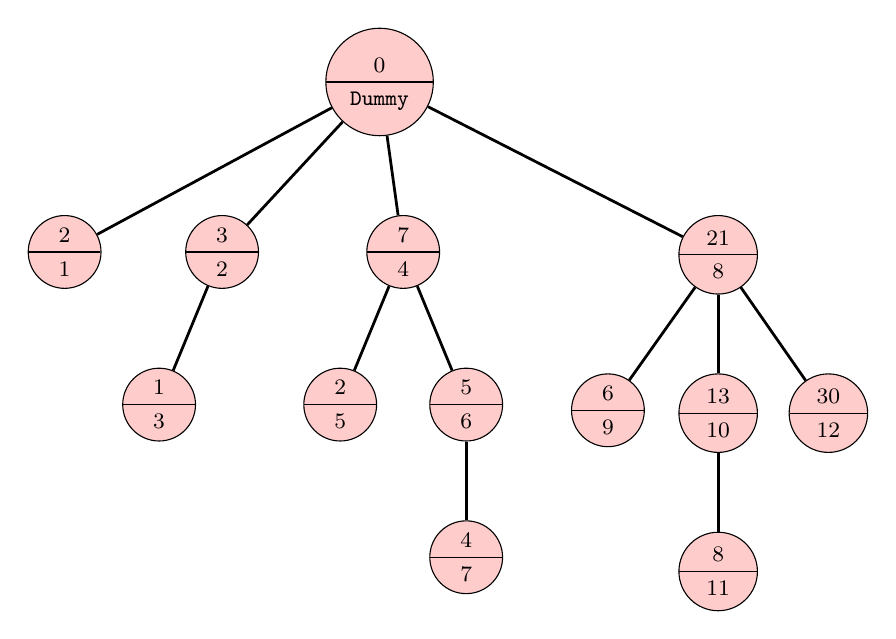
\begin{tikzpicture}
[my/.style={draw, circle split, fill=red!20!}]
\node[my](0){\footnotesize {$ 0 $}\nodepart{lower}{\footnotesize \texttt{Dummy}}};
\node[my](1)[below=1cm of 0, xshift=-4cm]{\footnotesize {$ 2 $}\nodepart{lower}{\footnotesize $ 1 $}};
\node[my](2)[below=1cm of 0, xshift=-2cm]{\footnotesize {$ 3 $}\nodepart{lower}{\footnotesize $ 2 $}};
\node[my](3)[below=1cm of 0, xshift=3mm]{\footnotesize {$ 7 $}\nodepart{lower}{\footnotesize $ 4 $}};
\node[my](4)[below=1cm of 0, xshift=4.3cm]{\footnotesize {$ 21 $}\nodepart{lower}{\footnotesize $ 8 $}};
\node[my](5)[below=1cm of 2, xshift=-8mm]{\footnotesize {$ 1 $}\nodepart{lower}{\footnotesize $3$}};
\node[my](6)[below=1cm of 3, xshift=-8mm]{\footnotesize {$ 2 $}\nodepart{lower}{\footnotesize $ 5 $}};
\node[my](7)[below=1cm of 3, xshift=8mm]{\footnotesize {$ 5 $}\nodepart{lower}{\footnotesize $ 6 $}};
\node[my](8)[below=1cm of 4, xshift=-1.4cm]{\footnotesize {$ 6 $}\nodepart{lower}{\footnotesize $ 9 $}};
\node[my](9)[below=1cm of 4]{\footnotesize {$ 13 $}\nodepart{lower}{\footnotesize $ 10 $}};
\node[my](10)[below=1cm of 4, xshift=1.4cm]{\footnotesize {$ 30 $}\nodepart{lower}{\footnotesize $ 12 $}};
\node[my](11)[below=1cm of 7]{\footnotesize {$ 4 $}\nodepart{lower}{\footnotesize $ 7 $}};
\node[my](12)[below=1cm of 9]{\footnotesize {$ 8 $}\nodepart{lower}{\footnotesize $ 11 $}};
\draw[line width=1pt] (0)--(1);
\draw[line width=1pt] (0)--(2);
\draw[line width=1pt] (0)--(3);
\draw[line width=1pt] (0)--(4);
\draw[line width=1pt] (2)--(5);
\draw[line width=1pt] (3)--(6);
\draw[line width=1pt] (3)--(7);
\draw[line width=1pt] (4)--(8);
\draw[line width=1pt] (4)--(9);
\draw[line width=1pt] (4)--(10);
\draw[line width=1pt] (7)--(11);
\draw[line width=1pt] (9)--(12);
\end{tikzpicture}
\end{figure}
其中
\begin{itemize}
\item $B[0]$ 是dummy node
\item $B[y]$ is the parent of $B[x]$ if $y=x-(x\land(-x))$
\item $ B[y] $的子节点$ B[x] $保存的是$A[y\ldots x]$的sum。
\end{itemize}
对于Update操作,即update index $i$ by adding a value $t$ or $A[i]\gets A[i]+t$,算法大致步骤如下
\begin{enumerate}
\item 同样从从index $i = L+1$开始进行循环,其中$L$是$ A $的长度。
\item 在循环的每一步:
\begin{itemize}
\item Update $B[i]$ as $B[i] + t$
\item Go to parent of $ B[i] $,这里$ B[i] $的parent是通过incrementing the last 1 bit of current index $ i $得到的,即$i\gets i + (i\land(-i))$。
\end{itemize}
\end{enumerate}
\subsubsection{How does Binary Indexed Tree work?}
\begin{itemize}
\item The idea is based on the fact that all positive integers can be represented as the sum of powers of 2。例如19可以表示成$19=16+2+1$。
\item BIT中的每个node保存的是sum of $n$ elements where n is a power of 2。例如,在上述示意图中,the sum of the first 12 elements 可以分为两个部分
\begin{enumerate}
\item The sum of the last 4 elements (from 9 to 12)。
\item The sum of the first 8 elements (from 1 to 8)。
\end{enumerate}
\item 而number $ n$对应的二进制数中bit 1的个数是$ \lceil\log n\rceil $。因此上述两个操作最多只需要遍历$ \lceil\log n\rceil $ nodes。
\item 构建$BIT$的时间复杂度为$ O(n\log n) $,因为需要call update operation for all $ n $ elements。
\end{itemize}
相关的算法如下:
\begin{enumerate}
\item Get sum of $A[0\ldots i]$
\setcounter{algorithm}{0}
\begin{algorithm}[H]
\caption{Get Sum of $ A[0\ldots i] $}
\begin{algorithmic}[1]
\Procedure{GetSum}{$B, i$}
\State $z:=0$
\State $i\gets i+1$ \Comment Index in $ B $ is 1 more than the one in $ A $
\While{$ i>0 $}
\State $z\gets z+B[i]$
\State $i\gets i - (i\land (-1))$ \Comment Move to the parent of $i$
\EndWhile 
\EndProcedure
\end{algorithmic}
\end{algorithm}
\item Update BIT by adding the given value $ d $ to $B[i+1]$ and all of its ancestors.
\begin{algorithm}[H]
\caption{Update BIT at index $ i+1 $ and all its ancestors}
\begin{algorithmic}[1]
\Procedure{Update}{$ B, L, i, d $}
\State $i\gets i+1$ \Comment Change to index in $B$
\While{$i \leq L-1$} \Comment $L-1$ is the length of original array
\State $ B[i]\gets B[i] + d $ \Comment Add $ d $ to current node of BIT
\State $ i\gets i + i\land(-i)  $
\EndWhile
\EndProcedure
\end{algorithmic}
\end{algorithm}
\item Contruct BIT, suppose the input array $A$ has size $ n $
\begin{algorithm}[H]
\caption{Construct BIT}
\begin{algorithmic}[1]
\Procedure{Construct}{$ A, n $}
\State $\star$ 创建一个大小为$ n+1 $的数组$B$作为BIT,同时初始化所有元素为零
\State $\ast$ Call \texttt{Update} by adding $A[i]$ to $B[i+1]$ and all of its ancetors
\For{$i:=0$ \textbf{to} $ n-1 $}
\State \Call{Update}{$ B, n+1, i, A[i] $}
\EndFor 
\State \Return $ B $
\EndProcedure
\end{algorithmic}
\end{algorithm}
\end{enumerate}
运用到本题中,要注意到\texttt{Update}中,输入的$d$其实是$A[i]$的增量。而在本题中,value是$A[i]$update之后的值,所以$d$就是$ A[i] $前后的插值。
\setcounter{lstlisting}{0}
\begin{lstlisting}[style=customc, caption={BIT}]
class NumArray
{
public:
    NumArray( vector<int> nums )
    {

        int n = static_cast<int>( nums.size() );

        vector<int> tmp( n + 1, 0 );

        swap( tmp, BIT );

        swap( A, nums );

        //Construct BIT
        for( int i = 0; i < n; ++i )
        {
            updateBIT( i, A[i] );
        }

    }

    //update BIT for the changes values in A[i]
    void updateBIT( int i, int diff )
    {
        int x = i + 1;
        int n = static_cast<int>( A.size() );

        while( x <= n )
        {
            BIT[x] += diff;
            x += ( x & ( -x ) );
        }
    }

    //val is the value that A[i] will be updated to
    //not the different
    void update( int i, int val )
    {

        int diff = val - A[i];

        //Don't forget to update A[i]
        A[i] = val;

        updateBIT( i, diff );

    }

    int getSum( int i )
    {
        int x = i + 1;

        int sum = 0;

        while( x > 0 )
        {
            sum += BIT[x];

            x -= ( x & ( -x ) );
        }

        return sum;
    }

    int sumRange( int i, int j )
    {

        int s1 = getSum( i - 1 );
        int s2 = getSum( j );

        return s2 - s1;
    }


    vector<int> BIT;

    vector<int> A;
};

\end{lstlisting}
\subsection{Segment Tree}
这是range sum最典型的数据结构,其中
\begin{itemize}
\item 叶子节点是输入数组的elements.
\item Each internal node represents some merging of the leaf nodes. The merging are different for different problems. 对于本题, merging 则代表 the sum of leaves under a node.
\item Segment Trees一般用array来代表。For each node at index $i$, the left child is at index $2\times i+1$, right child at $2\times i+2$ and the parent is at $ \lfloor (i-1)/2\rfloor $ 
\item 和Heap不同,Segment Tree不是完全二叉树,只是full binary tree,即每个node有0或者2 nodes。
\end{itemize}
具体的算法包括Construct,Query和Update。
\begin{itemize}
\item Construction:
\begin{enumerate}
\item Start the whole array $A[0\ldots L-1]$ as the first segment
\item Every time, 如果当前segment的length不为1,则将其对半划分为两个部分,然后对这两个部分继续下一层递归。
\end{enumerate}
\begin{itemize}
\item 由于构建出的tree是full binary tree with $ n $ leaves,因此总共有$ n-1 $ internal nodes。这样total nodes有$ 2\times n -1 $。
\item Tree的高度为$ \lceil log_2{n}\rceil $。总共需要分配大小为$ 2\times 2^{\lceil log_2{n}\rceil}-1 $的memory。
\end{itemize}
\begin{algorithm}[H]
\caption{Segment Tree Construction}
\begin{algorithmic}[1]
\Procedure{Construct}{$ A, n $} \Comment Input array $A$ has size $n$
\State $\star$ 创建大小为$ 2\times 2^{\lceil log_2{n}\rceil}-1 $的array $T$ 作为 Segment Tree
\State $\ast$ Call helper function to recursively building segment tree $T$ from $T[0]$ for range $A[0\ldots n-1]$
\State \Call{ConstructUtil}{$ A, 0, n-1, T, 0 $} 
\EndProcedure
\end{algorithmic}
\end{algorithm}

\begin{algorithm}[H]
\caption{Construct Helper Function To Recursively Building Segment Tree}
\begin{algorithmic}[1]
\Procedure{ConstructUtil}{$ A, l, r, T, x $}
\State $\ast$ Build leaf node
\If{$l=r$}
\State $T[x]\gets A[l]$
\State \Return $T[x]$
\EndIf
\State $m:=(l+r)/2$ \Comment 对半划分$ A[l\ldots r]$
\State $\ast$ Recursively building left substree for $A[l\ldots m]$
\State $\ast$ 这时候$T[x]$的left child node is $2\times x+1$
\algstore{307algo}
\end{algorithmic}
\end{algorithm}
\begin{algorithm}[H]
\begin{algorithmic}[1]
\algrestore{307algo}
\State $s_0:=$\Call{ConstructUtil}{$ A, l, m, T, 2\times x+1 $}
\State $\ast$ Recursively building right substree for $A[m+1\ldots r]$
\State $\ast$ 这时候$T[x]$的right child node is $2\times x+2$
\State $s_1:=$\Call{ConstructUtil}{$ A, m+1, r, T, 2\times x+2 $}
\State $\ast$ Merge left and right subtree results (Here is the sum)
\State $T[x]\gets s_0+s_1$
\State \Return $T[x]$
\EndProcedure
\end{algorithmic}
\end{algorithm}
\item Query: Suppose we want to query the range sum of $A[l\ldots r]$, and the segment tree is $T$.  Since $T[0]$ contains the range sum of $A[0,n-1]$($n$ is the size of $A$), the recursion starts with $T[0]$ for range $[0,n-1]$.
\begin{itemize}
\item Notice: In the algorithm, we don't need $A$.
\end{itemize}
\begin{algorithm}[H]
\caption{Get Range Sum For Segment Tree}
\begin{algorithmic}[1]
\Procedure{GetSum}{$T, n, l, r, 0$}
\If{$l > n-1$ \textbf{or} $r < 0$} \Comment Query range $ [l\ldots r] $ is outside of $[0\ldots n-1]$
\State \Return An invalid result
\EndIf
\State $\ast$ The recursion starts with $T[0]$ for range $[0,n-1]$.
\State \Return \Call{GetSumUtil}{$ T, 0, n-1, l, r, 0 $}
\EndProcedure
\end{algorithmic}
\end{algorithm}
\begin{algorithm}[H]
\caption{Helper Function To Get Range Sum}
\begin{algorithmic}[1]
\Procedure{GetSumUtil}{$T, \alpha, \beta ,l, r, x$}
\State $\ast$ Check if range $ [\alpha,\beta] $ is completely contained by the query range $ [l,r] $
\If{ $\alpha \geq l$ \textbf{and} $ \beta \leq r $ }
\State Node $x$ of $T$ has the sum for range $ [l,r] $
\State \Return $ T[x] $
\ElsIf{$\beta<l$ \textbf{or} $ \alpha > r $} \Comment Range $ [\alpha,\beta] $ does not overlap with the query range $ [l,r] $
\State \Return 0 \Comment We must return 0
\Else \Comment Range $ [\alpha,\beta] $ does not overlap with the query range $ [l,r] $
\algstore{307algo}
\end{algorithmic}
\end{algorithm}
\begin{algorithm}[H]
\begin{algorithmic}[1]
\algrestore{307algo}
\State $\ast$ 分别对$ T[i] $的left and right child node进行递归。
\State $m:=(\alpha+\beta)/2$
\State $\ast$ Recursively process the left child tree of $T[x]$
\State $s_0:=$\Call{GetSumUtil}{$ T, \alpha, m, l ,r, 2\times x + 1 $}
\State $\ast$ Recursively process the right child tree of $T[x]$
\State $s_1:=$\Call{GetSumUtil}{$ T, m+1, \beta, l ,r, 2\times x + 2 $}
\State $\ast$ Merge the result (here is the sum)
\State \Return $s_0 + s_1$
\EndIf
\EndProcedure
\end{algorithmic}
\end{algorithm}
\item Update:  Suppose we are updating $A[i]$ to V. 
\begin{enumerate}
\item Starts from root of the segment tree and add $ \delta:= V-A[i] $ to all nodes which have given index $ i $ in their range.
\item If a node does not have given index $ i $ in its range, no any change to this node.
\end{enumerate}
\begin{algorithm}[H]
\caption{Update Segment Tree When $A[i]$ is updated to $V$}
\begin{algorithmic}[1]
\Procedure{Update}{$ T, A, n, i, V$}
\State $\star$ Make sure $i$ is inside $[0,n-1]$
\State $\delta:=V-A[i]$
\State $\ast$ The recursion starts with $T[0]$ for range $[0,n-1]$.
\State \Call{UpdateUtil}{$ T, 0, n-1, i, 0, \delta $}
\EndProcedure
\end{algorithmic}
\end{algorithm}
\begin{algorithm}[H]
\caption{Helper Function: $A[i]$ is updated to $A[i]+\delta$}
\begin{algorithmic}[1]
\Procedure{UpdateUtil}{$ T, \alpha, \beta, i, x, \delta $}
\State $\ast$ If $i$ lies outside of range $[\alpha, \beta]$, just return
\If{$i>\beta$ \textbf{or} $ i<\alpha $}
\State \Return
\EndIf
\State $T[x]\gets T[x]+\delta$ \Comment Update node $x$ of segment tree $T$
\algstore{307algo}
\end{algorithmic}
\end{algorithm}
\begin{algorithm}[H]
\begin{algorithmic}[1]
\algrestore{307algo}
\If{$\alpha \neq \beta$} \Comment \textbf{Important}: the range must have at least two elements
\State $m:=(\alpha+\beta)/2$
\State $\ast$ Update left subtree of $T[x]$
\State \Call{Update}{$ T, \alpha, m, i , 2\times x+1, \delta $} 
\State $\ast$ Update right subtree of $T[x]$
\State \Call{Update}{$ T, m+1, \beta, i , 2\times x+2, \delta $} 
\EndIf
\EndProcedure
\end{algorithmic}
\end{algorithm}
\end{itemize}
用Segment Tree作为本题的Solution的代码如下
\begin{lstlisting}[style=customc, caption={Solution Code With Segment Tree}]
class NumArray
{
public:
    NumArray( vector<int> nums )
    {
        if( nums.empty() )
        {
            return;
        }

        swap( A, nums );


        int n = static_cast<int>( A.size() );

        //This is the height of the segment tree
        int h = static_cast< int >( log2( n ) + 1 );
        //The size of the segment tree
        int sz = ( 1 << ( h + 1 ) ) - 1;

        vector<int> tmp( sz, 0 );

        swap( tmp, st );

        //Build Segment Tree
        buildUtil( 0, n - 1, 0 );
    }

    int buildUtil( int start, int end, int ti )
    {
        if( start == end )
        {
            st[ti] = A[start];
            return st[ti];
        }

        int mid = ( start + end ) / 2;
        int l = buildUtil( start, mid, 2 * ti + 1 );
        int r = buildUtil( mid + 1, end, 2 * ti + 2 );

        st[ti] = l + r;
        return st[ti];
    }


    void updateUtil( int start, int end, int a_pos, int diff, int t_pos )
    {
        if( ( a_pos < start ) || ( a_pos > end ) )
        {
            return;
        }

        st[t_pos] += diff;

        //Very important:
        //Stop update when start = end
        if( start != end )
        {
            int mid = ( start + end ) / 2;

            updateUtil( start, mid, a_pos, diff, t_pos * 2 + 1 );
            updateUtil( mid + 1, end, a_pos, diff, t_pos * 2 + 2 );
        }

    }

    void update( int i, int val )
    {
        int n = static_cast<int>( A.size() );

        if( ( i < 0 ) || ( i > n - 1 ) )
        {
            return;
        }

        int diff = val - A[i];

        A[i] = val;

        updateUtil( 0, n - 1, i, diff, 0 );
    }

    int getSum( int start, int end, int i, int j, int ti )
    {
        //if the given range [i,j] include [start, end]
        //return the number in st[ti]
        if( ( start >= i ) && ( end <= j ) )
        {
            return st[ti];
        }

        //[i,j] does not overlap with [start, end]
        if( ( start > j ) || ( end < i ) )
        {
            //Return 0 since we cannot get
            //any value for this range
            return 0;
        }

        int mid = ( start + end ) / 2;

        int l = getSum( start, mid, i, j, ti * 2 + 1 );
        int r = getSum( mid + 1, end, i, j, ti * 2 + 2 );

        return l + r;
    }

    int sumRange( int i, int j )
    {
        int n = static_cast<int>( A.size() );

        if( ( j < 0 ) || ( i > n - 1 ) )
        {
            return -1;
        }


        return getSum( 0, n - 1, i, j, 0 );
    }

    vector<int> st;
    vector<int> A;
};

\end{lstlisting}
\subsection{Iterative Segment Tree}
上述代码中,Segment Tree的内存空间有很多浪费,实际上可以把Segment Tree的内存压缩的更多,这样就是iterative segment tree的实现方法
\begin{itemize}
\item 这种方法中,segment tree的array的大小为$2\times N$,其中$N$是输入数组的大小。

\item The leaf nodes start from index $N$ and go up to index $ 2\times N -1 $。因此,$A[i]$在segment tree array中的index为$ i+N $o
\item 如果要得到某个element的parents,就要从index $ N-1 $出发,move upward。Now to calculate the parents, we will start from index (N – 1) and move upward. 
\item For an index $ i $, its left child is at $ 2\times i $ and right child will be at $ 2\times i + 1 $ index。 So the values at nodes $ 2\times i $ and $ 2\times i + 1 $ is combined at $i$th node to construct the tree.
\end{itemize}
实现算法伪代码如下,首先是build
\begin{algorithm}[H]
\caption{Iterativly Build Segment Tree}
\begin{algorithmic}[1]
\Procedure{Build}{$A, n, T$}
\For{$i:=0$ \textbf{to} $ n-1 $}
\State $ T[i+n]\gets A[i] $ \Comment Leaf nodes
\EndFor
\For{$i:=n-1$ \textbf{to} $ 0 $}
\State $ T[i]\gets T[i\times 2] + T[i\times 2 +1] $ \Comment Leaf nodes
\EndFor
\EndProcedure
\end{algorithmic}
\end{algorithm}
下面的是update,其中$p$为index in $A$ to be updated,$v$为update后的value。
\begin{algorithm}[H]
\caption{Iterativly Update Segment Tree}
\begin{algorithmic}[1]
\Procedure{Update}{$A, n, p, v, T$}
\State $\ast$ Set value at position $p$ to $v$
\State $ T[p+n]\gets v$
\State $i:=p+n$
\State $\ast$ Move upwards and update parents
\State $\star$ 由于$T[0]$是dummy node,因此循环只需要到$i=1$即可
\While{$i > 1$}
\State $\ast$ If $i$ is odd, the left child is $ i-1 $ and the right child $ i $
\State $\ast$ If $i$ is even, the right child is $ i+1 $ and the left child is $ i $
\State $ T[i/2] = T[i] + T[i \oplus 1] $
\State $i\gets i /2 $
\EndWhile
\EndProcedure
\end{algorithmic}
\end{algorithm}
The idea behind the query function is that whether we should include an element in the sum or we should include its parent.
\begin{itemize}
\item Suppose range of query is $ [l, r] $
\item Check $l$ 是不是其parent $ P $的right child,即$l$是不是odd number。
\begin{enumerate}
\item 如果$l$是odd number,显然$l$是其parent $ P $的right child,parent $ P $ 的
range sum中包含的是$ l $的range sum,和另外一个child的range sum。而这个child 是落在range $ [l,r] $之外的。因此结果中不需要$P$的range sum,而只需要$l$的range sum。然后move $ l $到$P$的下一个node,即$l\gets (l+1)/2$。
\item 如果$ l $是even number, 它是其parent $ P $的left child。 parent $ P $ 的 range sum就落在 range $[l,r]$中,只需要将 $ l $ move 到 $ P $,即$l\gets l/2$。
\end{enumerate}
\item 类似的,Check $r$ 是不是其parent $ P $的left child,即$r$是不是even number。
\begin{enumerate}
\item 如果$r$是even number,显然$r$是其parent $ P $的left child,parent $ P $ 的
range sum中包含的是$ r $的range sum,和另外一个child的range sum。而这个child 是落在range $ [l,r] $之外的。因此结果中不需要$P$的range sum,而只需要$r$的range sum。然后move $ r $到$P$的上一个node,即$r\gets (r-1)/2$。
\item 如果$ r $是odd number, 它是其parent $ P $的right child。 parent $ P $ 的 range sum就落在 range $[l,r]$中,只需要将 $ r $ move 到 $ P $,即$r\gets r/2$。
\end{enumerate}
\end{itemize}
\begin{algorithm}[H]
\caption{Iterative Segement Tree Query}
\begin{algorithmic}[1]
\Procedure{Query}{A, L, l, r, T}
\State $x\gets x+n$ \Comment The leaf node of $l$
\State $y\gets y+n$ \Comment The leaf node of $r$
\State $z:=0$ \Comment The range sum
\While{$l \leq r$}
\If{$l$ is odd number} \Comment $l$ is the right child of its parent
\State $z\gets z + T[l]$
\State $l\gets (l+1)/2$ \Comment Move $l$ to its parent's right node
\Else
\State $l\gets l/2$
\EndIf
\If{$r$ is even number} \Comment $r$ is the left child of its parent
\State $z\gets z + T[r]$
\State $r\gets (r-1)/2$ \Comment Move $l$ to the left node of its parent
\Else
\State $r\gets r/2$
\EndIf
\EndWhile
\State \Return $ z $
\EndProcedure
\end{algorithmic}
\end{algorithm}
\begin{lstlisting}[style=customc, caption={Iteratively Segement Tree}]
class NumArray
{
public:
    NumArray( vector<int> nums )
    {
        if( nums.empty() )
        {
            return;
        }

        swap( A, nums );

        vector<int> tmp( A.size() * 2, 0 );
        swap( tmp, T );

        //build segment tree
        build();
    }

    void build()
    {
        auto n = static_cast<int>( A.size() );

        //set leaf nodes
        for( int i = 0; i < n; ++i )
        {
            T[n + i] = A[i];
        }

        //set parent nodes
        for( int i = n - 1; i > 0; --i )
        {
            T[i] = T[i * 2] + T[i * 2 + 1];
        }
    }

    void update( int i, int val )
    {
        auto n = static_cast<int>( A.size() );

        //update leaf node
        T[i + n] = val;

        int x = i + n;

        //update parent nodes
        //since T[0] is dummy node
        //the loop runs until x=1
        while( x > 1 )
        {
            T[x / 2] = T[x] + T[x ^ 1];
            x = x / 2;
        }
    }

    int sumRange( int i, int j )
    {
        auto n = static_cast<int>( A.size() );

        int x = i + n;
        int y = j + n;

        int sum = 0;

        while( x <= y )
        {
            if( x & 1 )
            {
                //x is the right child of its parent
                sum += T[x];
                //move x to the right of its parent node
                //through x/=2 outside
                ++x;
            }

            if( ( y & 1 ) == 0 )
            {
                //y is the left child of its parent
                sum += T[y];
                //move y to the left of its parent node
                //through y/=2 outside
                --y;
            }

            x /= 2;
            y /= 2;
        }

        return sum;
    }

    vector<int> A;
    vector<int> T;
};


\end{lstlisting}
% \section{308 --- Range Sum Query 2D - Mutable}
Given a 2D matrix matrix $M$, find the sum of the elements inside the rectangle defined by its upper left corner $(r_1, c_1)$ and lower right corner $(r_2, c_2)$.
\begin{figure}[H]
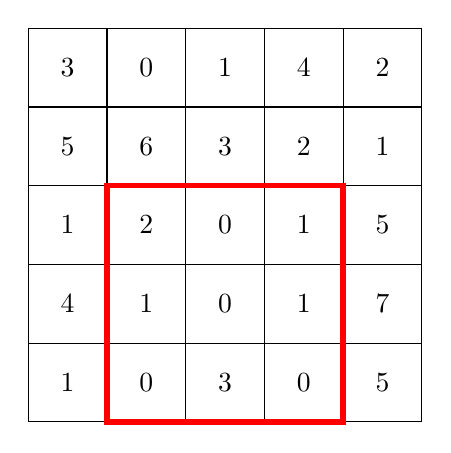
\begin{tikzpicture}
\draw[black, thin] (0,0) grid (5,5);
\node at (0.5,4.5) {$3$};
\node at (1.5,4.5) {$0$};
\node at (2.5,4.5) {$1$};
\node at (3.5,4.5) {$4$};
\node at (4.5,4.5) {$2$};
%row2
\node at (0.5,3.5) {$5$};
\node at (1.5,3.5) {$6$};
\node at (2.5,3.5) {$3$};
\node at (3.5,3.5) {$2$};
\node at (4.5,3.5) {$1$};
%row3
\node at (0.5,2.5) {$1$};
\node at (1.5,2.5) {$2$};
\node at (2.5,2.5) {$0$};
\node at (3.5,2.5) {$1$};
\node at (4.5,2.5) {$5$};
%row 4
\node at (0.5,1.5) {$4$};
\node at (1.5,1.5) {$1$};
\node at (2.5,1.5) {$0$};
\node at (3.5,1.5) {$1$};
\node at (4.5,1.5) {$7$};
%row 5
\node at (0.5,0.5) {$1$};
\node at (1.5,0.5) {$0$};
\node at (2.5,0.5) {$3$};
\node at (3.5,0.5) {$0$};
\node at (4.5,0.5) {$5$};
\draw[line width=2pt,red] (1,0) rectangle ++(3,3);
\end{tikzpicture}
\end{figure}
The above rectangle (with the red border) is defined by $(r_1, c_1) = (2, 1)$ and $(r_2, c_2) = (4, 3)$, which contains sum = 8.
\paragraph{Example:}
\begin{flushleft}
Give matrix $M$ is
\begin{table}[H]
    \begin{tabular}{ccccc}
        3 & 0 & 1 & 4 & 2 \\
        5 &  6 &  3 &  2 &  1\\
        1 &  2 &  0 &  1 &  5 \\
        4 &  1 &  0 &  1 &  7\\
        1 &  0 &  3 &  0 &  5
    \end{tabular}
\end{table}
\begin{lstlisting}[style=customc]
sumRegion(2, 1, 4, 3); // 8
update(3, 2, 2);
sumRegion(2, 1, 4, 3); // 10
\end{lstlisting}
\end{flushleft}

\paragraph{Note:}
\begin{itemize}
\item The matrix is only modifiable by the update function.
\item You may assume the number of calls to \texttt{update} and \texttt{sumRegion} function is distributed evenly.
 \item You may assume that $r_1 \leq r_2$ and $c_1 \leq c_2$.
\end{itemize}
\subsection{2D BIT}
\begin{itemize}
\item 为了快速update 二维区域,还是采用BIT的数据结构,但是是2D,即row和column分别按照BIT进行build。算法和一维的没有区别。
\item 与1维的BIT类似, 2D BIT也是只能得到从$ (0,0) $到 $ (r,c) $的区间和,因此需要按照304中的分区域计算方法,分别计算出四个角的区域和。
\item 如果$M$的dimension为$m\times n$,与1维的BIT类似,2维的BIT的dimension is equal to $ (m+1)\times (n+1) $
\end{itemize}
假设$M[r][c]$的值变化了$\delta$,那么BIT的update算法如下
\setcounter{algorithm}{0}
\begin{algorithm}[H]
\caption{Update BIT}
\begin{algorithmic}[1]
\Procedure{UpdateBIT}{$M, m, n, B, r,c,\delta$}
\State $x:=r+1$
\While{$x \leq m$}
\State $y:=c+1$ \Comment Note: y must be reset to $ c+1 $ at each iteration of $ x $
\While{$ y \leq n $}
\State $ B[x][y]\gets B[x][y] + \delta $
\State $y\gets y + (y\land (-y))$ \Comment Move $y$ to its child node
\EndWhile
\State $x\gets x + (x\land (-x))$ \Comment Move $x$ to its child node
\EndWhile
\EndProcedure
\end{algorithmic}
\end{algorithm}
计算range sum from $ (0,0) $ to $ (r,c) $的算法如下,算法中并不需要$M$。
\begin{algorithm}[H]
\caption{Get Range Sum From BIT}
\begin{algorithmic}[1]
\Procedure{GetSum}{$B, r, c$}
\State $x:=r+1$
\State $z:=0$ \Comment The total sum
\While{$x>0$}
\State $y:=c+1$ \Comment Note: y must be reset to $ c+1 $ at each iteration of $ x $
\While{$ y>0 $}
\State $z\gets z+B[x][y]$
\State $y\gets y - (y\land (-y))$ \Comment Move $y$ to its parent node
\algstore{308algo}
\end{algorithmic}
\end{algorithm}
\begin{algorithm}[H]
\begin{algorithmic}[1]
\algrestore{308algo}
\EndWhile
\State $x\gets x - (x\land (-x))$ \Comment Move $x$ to its parent node
\EndWhile
\State \Return $ z $
\EndProcedure
\end{algorithmic}
\end{algorithm}
\setcounter{lstlisting}{0}
\begin{lstlisting}[style=customc, caption={BIT}]
class NumMatrix
{
public:
    NumMatrix( vector<vector<int>> &matrix )
        : M( matrix )
    {
        vector<vector<int>> tmp( M.size() + 1, vector<int> ( M[0].size() + 1, 0 ) );

        swap( tmp, BIT );

        m = static_cast< int >( M.size() );
        n = static_cast< int >( M[0].size() );

        for( int r = 0; r < m; ++r )
        {
            for( int c = 0; c < n; ++c )
            {
                updateBIT( r, c, M[r][c] );
            }
        }
    }

    void update( int row, int col, int val )
    {
        int diff = val - M[row][col];

        updateBIT( row, col, diff );
    }

    int sumRegion( int row1, int col1, int row2, int col2 )
    {
        //Four regions computation
        return sumBIT( row2, col2 )
               - sumBIT( row1 - 1, col2 )
               - sumBIT( row2, col1 - 1 )
               + sumBIT( row1 - 1, col1 - 1 );
    }

private:

    void updateBIT( int r, int c, int diff )
    {
        int x = r + 1;

        while( x <= m )
        {
            //must reset y at each iteration
            int y = c + 1;

            while( y <= n )
            {
                BIT[x][y] += diff;

                y += ( y & ( -y ) );
            }

            x += ( x & ( -x ) );
        }
    }

    int sumBIT( int r, int c )
    {
        int x = r + 1;

        int sum = 0;

        while( x > 0 )
        {
            //must reset y at each iteration
            int y = c + 1;

            while( y > 0 )
            {
                sum += BIT[x][y];
                y -= ( y & ( -y ) );
            }

            x -= ( x & ( -x ) );
        }

        return sum;
    }

    vector<vector<int>>& M;
    vector<vector<int>> BIT;

    int m;
    int n;
};
\end{lstlisting}
% \section{309 --- Best Time to Buy and Sell Stock with Cooldown}
Say you have an array $A$ for which the $ i $th element is the price of a given stock on day $ i $.
\par
Design an algorithm to find the maximum profit. You may complete as many transactions as you like (ie, buy one and sell one share of the stock multiple times) with the following restrictions:
\par
You may not engage in multiple transactions at the same time (ie, you must sell the stock before you buy again).
\par
After you sell your stock, you cannot buy stock on next day. (ie, cooldown 1 day)

\paragraph{Example:}

\begin{flushleft}
\textbf{Input}: $ [1,\;2,\;3,\;0,\;2] $
\\
\textbf{Output}: 3 
\\
\textbf{Explanation}: transactions = [\texttt{buy}, \texttt{sell}, \texttt{cooldown}, \texttt{buy}, \texttt{sell}]
\end{flushleft}
\subsection{Dynamic Programming}
在day $ i $,可以有如下四种选项
\begin{enumerate}
\item 手头有一个stock,然后卖出。
\item 手头有一个stock,然后什么都不做。
\item 手头没有stock,然后买入一股。
\item 手头没有stock,然后什么也不做。
\end{enumerate}
而这四个options在day $ i-1 $ 和 day $ i $是相关联的。
\begin{enumerate}
\item Choose option 1 in day $ i $,那么在 day $ i-1 $,可以 take option 2 和 3。
\item Choose option 2 on day $ i $,那么在 day $ i-1 $,可以 take option 2 和 3。
\item Choose option 3 on day $ i $,那么在 day $ i-1 $,只能 take option 4。因为有cooldown,所以不能够选择 option 1。
\item Choose option 3 on day $ i $,那么在 day $ i-1 $,可以 take option 1 和 4。
\end{enumerate}
由于不知道哪个option会带来最大的利润,因此需要尝试所有四个选项,然后选择能够带来最大利润的那个选项。例如,假设在day $ i $,选择了option 1。那么在day $ i-1 $,就要比较option 2和3哪个可以在 day $ i $ 产生最大的利润,这就需要靠DP方法来逐步计算。
\par
最开始在day 0时,各个选项的导致的profit的初始值如下
\begin{enumerate}
\item 由于最开始没有股票,需要买入,花费$A[0]$,而在当天又卖出,得到$A[0]$,这样实际的profit为0。
\item 由于最开始没有股票,需要买入,花费$A[0]$,然后什么都不做,因此profit 为$-A[0]$。
\item 与2一样,买入股票,花费$A[0]$,profit也是$-A[0]$。
\item 由于没有transaction,因此proift为0。
\end{enumerate}
在最后一天这四个option的最大值即为所能获得的最大profit。
\setcounter{lstlisting}{0}
\begin{lstlisting}[style=customc, caption={Dynamic Programming}]
int maxProfit( vector<int>& prices )
{
    if( prices.empty() || ( prices.size() == 1 ) )
    {
        return 0;
    }

    //H[0]: have stock and sell, H[1]: have stock and do nothing
    vector<int> H( 2, 0 );
    //U[0]: no stock and buy, U[1]: no stock and do nothing
    vector<int> U( 2, 0 );

    H[1] = -prices[0];//we must buy the stock and hold
    U[0] = -prices[0];//we must buy the stock


    for( size_t i = 1; i < prices.size(); ++i )
    {
        //save last day's values
        int tmp_h0 = H[0];
        int tmp_h1 = H[1];
        int tmp_u0 = U[0];
        int tmp_u1 = U[1];

        //The iterative relationship
        H[0] = ( max )( tmp_u0 + prices[i], tmp_h1 + prices[i] ); //1<-(2,3)
        H[1] = ( max )( tmp_u0, tmp_h1 ); //2<-(2,3)

        U[0] = tmp_u1 - prices[i]; //3<-4
        U[1] = ( max )( tmp_h0, tmp_u1 ); //4<-(1,4)
    }

    //The maximum profit is
    //the maximum value of these 4 variables
    int ans = max( H[0], H[1] );
    ans = ( max )( ans, U[0] );
    ans = ( max )( ans, U[1] );

    return ans;
}
\end{lstlisting}


\section{310 --- Minimum Height Trees}
For an undirected graph with tree characteristics, we can choose any node as the root. The result graph is then a rooted tree. Among all possible rooted trees, those with minimum height are called minimum height trees (MHTs). Given such a graph, write a function to find all the MHTs and return a list of their root labels.

\paragraph{Format}
\par
The graph contains $ n $ nodes which are labeled from 0 to $  n - 1 $. You will be given the number $ n $ and a list of undirected edges (each edge is a pair of labels).
\par
You can assume that no duplicate edges will appear in edges. Since all edges are undirected, $ [0, 1] $ is the same as $ [1, 0] $ and thus will not appear together in edges.

\paragraph{Example 1}:

\begin{flushleft}
\textbf{Input}: $ n = 4 $
\begin{figure}[H]
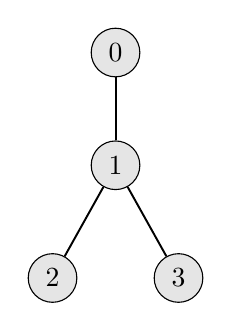
\begin{tikzpicture}
[my/.style={draw, circle, fill=gray!20!, minimum size=5mm}]
\node[my] (1) at (0,0) {0};
\node[my] (2) [below=8mm of 1] {1};
\node[my] (3) [below=8mm of 2, xshift=-8mm] {2};
\node[my] (4) [below=8mm of 2, xshift=8mm] {3};
\draw[line width=0.7pt] (1) -- (2);
\draw[line width=0.7pt] (2) -- (3);
\draw[line width=0.7pt] (2) -- (4);
\end{tikzpicture}
\end{figure}
\textbf{Output}: $ [1] $
\end{flushleft}

\paragraph{Example 2 :}

\begin{flushleft}
\textbf{Input}: $ n = 6 $
\begin{figure}[H]
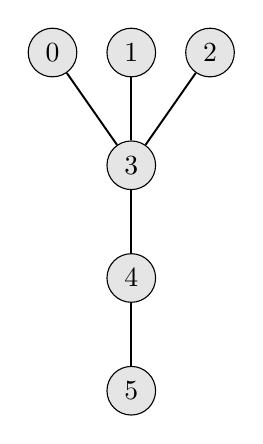
\begin{tikzpicture}
[my/.style={draw, circle, fill=gray!20!, minimum size=5mm}]
\node[my] (1) at (0,0) {3};
\node[my] (2) [above=8mm of 1] {1};
\node[my] (3) [above=8mm of 1, xshift=-1cm] {0};
\node[my] (4) [above=8mm of 1, xshift=1cm] {2};
\node[my] (5) [below=8mm of 1] {4};
\node[my] (6) [below=8mm of 5] {5};
\draw[line width=0.7pt] (1) -- (2);
\draw[line width=0.7pt] (1) -- (3);
\draw[line width=0.7pt] (1) -- (4);
\draw[line width=0.7pt] (1) -- (5);
\draw[line width=0.7pt] (5) -- (6);
\end{tikzpicture}
\end{figure}
\textbf{Output}: $ [3, 4] $
\end{flushleft}

\paragraph{Note:}

\begin{itemize}
\item According to the definition of tree on Wikipedia: \texttt{a tree is an undirected graph in which any two vertices are connected by \textit{exactly} one path. In other words, any connected graph without simple cycles is a tree}.
\item The height of a rooted tree is the number of edges on the longest downward path between the root and a leaf.
\end{itemize}
\subsection{Breadth First Search}
\begin{itemize}
\item 首先建立adjacent list的graph,然后创建一个queue,将所有只有degree为1即只有一个edge的节点放入队列中
\item 然后依次从queue中弹出节点$x$,将该节点从与之相连的节点$y$的adjacent list中删除。如果$y$的degree也变为了1,将$y$放入queue中。
\item 最后如果queue中的节点小于等于2,那么当前queue中的节点就是符合要求的root nodes。
\end{itemize}
\setcounter{lstlisting}{0}
\begin{lstlisting}[style=customc, caption={Breadth First Search}]
vector<int> findMinHeightTrees( int n, vector<pair<int, int>>& edges )
{
    if( n == 0 )
    {
        return {};
    }

    if( n == 1 )
    {
        return  {0};
    }

    //create adjacent list structure
    vector<unordered_set<int>> G( n );

    //This is an unordered graph
    for( const auto& edge : edges )
    {
        G[edge.first].insert( edge.second );
        G[edge.second].insert( edge.first );
    }

    queue<int> q;

    for( int i = 0; i < n; ++i )
    {
        if( G[i].size() == 1 )
        {
            //add all nodes with only edge
            q.emplace( i );
        }
    }

    vector<int> ans;

    //loop until there are no larger than 2 nodes in the queue
    while( n > 2 )
    {
        int q_size = static_cast< int >( q.size() );
        n -= q_size;

        for( int i = 0; i < q_size; ++i )
        {
            auto t = q.front();
            q.pop();

            //remove t from t's adjacent node lists
            int adj = *( G[t].begin() );
            G[adj].erase( t );

            if( G[adj].size() == 1 )
            {
                //t's adjacent also has degree 1 now
                q.push( adj );
            }
        }
    }

    //now nodes in queue are the
    //answer
    while( !q.empty() )
    {
        ans.push_back( q.front() );
        q.pop();
    }

    return ans;

}

\end{lstlisting}

\section{311 --- Sparse Matrix Multiplication}

\textbf{Medium}

Given two sparse matrices $A$ and $B$, return the result of $AB$.

You may assume that $A$'s column number is equal to $B$'s row number.

\paragraph{Example:}

\begin{flushleft}
\[
A = \begin{bmatrix}
1 & 0 & 0 \\
-1 & 0 & 3 \\
\end{bmatrix}
\]

\[
B = \begin{bmatrix}
7 & 0 & 0 \\
0 & 0 & 0 \\
0 & 0 & 1 \\
\end{bmatrix}
\]

\textbf{Output}:

\[
AB = \begin{bmatrix}
1 & 0 & 0 \\
-1 & 0 & 3 \\
\end{bmatrix} \times \begin{bmatrix}
7 & 0 & 0 \\
0 & 0 & 0 \\
0 & 0 & 1 \\
\end{bmatrix}
=\begin{bmatrix}
7 & 0 & 0 \\
-7 & 0 & 3 \\
\end{bmatrix}
\]


\end{flushleft}

\subsection{Skip Zero}
For matrix multiplication result $C$, 

\[
C[i]][j] = A[i][0]\times B[0][j] + A[i][1]\times B[1][j] + \ldots + A[i][k]\times B[k][j]
\]

Thus if $A[i][k]$ is zero, we can skip. Then we iterate over $k$th row of $B$. 

\setcounter{lstlisting}{0}
\begin{lstlisting}[style=customc, caption={Skip Zero}]
vector<vector<int>> multiply( vector<vector<int>>& A, vector<vector<int>>& B )
{
    vector<vector<int>> ans( A.size(), vector<int>( B[0].size(), 0 ) );
    for( size_t i = 0; i < A.size(); ++i )
    {
        for( size_t k = 0; k < A[i].size(); ++k )
        {
            if( A[i][k] )
            {
                for( size_t j = 0; j < B[0].size(); ++j )
                {
                    if( B[k][j] )
                    {
                        ans[i][j] += A[i][k] * B[k][j];
                    }
                }
            }
        }
    }
    return ans;
}
\end{lstlisting}

\paragraph{Related Problems}
\begin{itemize}
\item \textbf{264. Ugly Number II}
\end{itemize}
% \section{312 --- Burst Balloons}
Given $ n $ balloons, indexed from 0 to $ n-1 $. Each balloon is painted with a number on it represented by array nums. You are asked to burst all the balloons. If the you burst balloon i you will get nums[left] * nums[i] * nums[right] coins. Here left and right are adjacent indices of i. After the burst, the left and right then becomes adjacent.
\par
Find the maximum coins you can collect by bursting the balloons wisely.

\paragraph{Note:}

\begin{itemize}
\item You may imagine $A[-1] = A[n] = 1$. They are not real therefore you can not burst them.
$0 \leq n \leq 500$, $0 \leq A[i] \leq 100$
\end{itemize}

\paragraph{Example:}

\begin{flushleft}
\textbf{Input}: $[3,1,5,8]$
\\
\textbf{Output}: 167 
\\
\textbf{Explanation}: 
\begin{figure}[H]
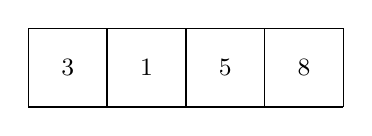
\begin{tikzpicture}
\draw[line width=0.5pt] (0,0) grid (4,1);
\node at (0.5,0.5) {{\small 3}};
\node at (1.5,0.5) {{\small 1}};
\node at (2.5,0.5) {{\small 5}};
\node at (3.5,0.5) {{\small 8}};
\end{tikzpicture}
\end{figure}
Burst ballon with number 1, get coins $=3\times 1\times5  $
\begin{figure}[H]
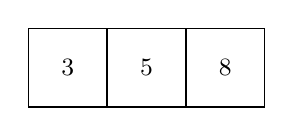
\begin{tikzpicture}
\draw[line width=0.5pt] (0,0) grid (3,1);
\node at (0.5,0.5) {{\small 3}};
\node at (1.5,0.5) {{\small 5}};
\node at (2.5,0.5) {{\small 8}};
\end{tikzpicture}
\end{figure}
Burst ballon with number 5, get coins $=3\times 5\times 8  $
\begin{figure}[H]
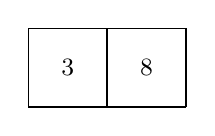
\begin{tikzpicture}
\draw[line width=0.5pt] (0,0) grid (2,1);
\node at (0.5,0.5) {{\small 3}};
\node at (1.5,0.5) {{\small 8}};
\end{tikzpicture}
\end{figure}
Burst ballon with number 3, get coins $=1\times 3\times  8  $
\begin{figure}[H]
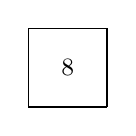
\begin{tikzpicture}
\draw[line width=0.5pt] (0,0) grid (1,1);
\node at (0.5,0.5) {{\small 8}};
\end{tikzpicture}
\end{figure}
Finally burst ballon with number 8, get coins $=1\times  8\times 1  $
\\
The total coins = $ 3\times 1\times5 + 3\times 5\times 8 +1\times 3\times  8 +1\times  8\times 1 = 167 $
\end{flushleft}
\subsection{Dynamic Programming}
\begin{itemize}
\item 这是一个2D dynamic programming。因此定义\texttt{DP} array $F[i][j]$表示the maximum coins by bursting all ballons from $ A[i] $ to $ A[j] $。
\item 这里有个trick的点,即$F[i][j]$是burst all ballons from $ A[i] $ to $ A[j] $,这意味着在$ [i,j] $中的某个index $ k $,如果计算出$ F[i][k-1] $和 $ F[k+1][j] $,也就意味着 $ A[i] $和$ A[j] $就不再和$ A[k] $相邻了。这时候$ A[k] $的左右边两边的ballon分别是$ A[i-1] $和$ A[j+1] $了。
\item 基于上述分析,对于$ [i,j] $中的某个index $ k $,即$ i\leq k\leq j $,如果选择burst $A[k]$,那么所获得的maximum coins为$F[i][k-1] + F[k+1][j] + A[i-1]\times A[k]\times A[j+1]$。所以$ F][j] = \max(\underbrace{F[i][k-1] + F[k+1][j] + A[i-1]\times A[k]\times A[j+1]}_{i\leq k\leq j}$
\item 由于$i\leq k\leq j$,那么当$k=i$或者$k=j$时,会出现$ F[i][i-1] $和$ F[j+1][j] $,这个是$F$的左下三角,而$ F $的更新都在右上三角,初始化时都设为零,因此不会有问题。
\item 另外,当只有一个元素的时候,$ F $的递推会越界,为了解决这个问题,在$ A $的前后分别加上1。然后$F$的dimension为$ (L+2)\times(L+2) $。最后返回$F[1][L]$ ($ L $ is the size of $ A $)。
\item 在进行$ F $递推时,最外层循环当前更新的长度$ \ell $,从1到$ L $,而内层循环的$l$则从1开始,因为我们已经插入了1在最前面。同样$ l $循环到$l+\ell-1 = L$为止,因为也插入了1在最后面。
\end{itemize}
\setcounter{lstlisting}{0}
\begin{lstlisting}[style=customc, caption={Dynamic Programming}]
int maxCoins( vector<int>& nums )
{
    int sz = static_cast<int>( nums.size() );

    //Add 1 to begin and end of A
    vector<int> A( nums.size() + 2, 1 );

    auto it = A.begin();
    ++it;

    copy( nums.begin(), nums.end(), it );

    vector<vector<int>> F( sz + 2, vector<int>( sz + 2, 0 ) );

    //Filling the up right triangle of F
    for( int l = 1; l <= sz; ++l )
    {
        for( int x = 1; x + l - 1 <= sz; ++x )
        {
            int y = x + l - 1;

            for( int k = x; k <= y; ++k )
            {
                //All ballons from A[x] to A[y] are bursted
                //A[k] is adjacent to A[x-1] and A[y+1]
                int coins = A[k] * A[x - 1] * A[y + 1];
                //burst all ballons from A[x] to A[k-1]
                coins += F[x][k - 1];
                //burst all ballons from A[k+1] to A[y]
                coins += F[k + 1][y];

                F[x][y] = ( max )( F[x][y], coins );
            }
        }
    }

    //F[1][sz] is the result for burst
    //all ballons from A[0] to A[sz-1]
    return F[1][sz];
}

\end{lstlisting}

\paragraph{Related Problems}
\begin{itemize}
\item \textbf{1000. Minimum Cost to Merge Stones}
\end{itemize}
\section{313 --- Super Ugly Number}

\textbf{Medium}

Write a program to find the $n$th super ugly number.

Super ugly numbers are positive numbers whose all prime factors are in the given prime list primes of size $k$.

\paragraph{Example:}

\begin{flushleft}
\textbf{Input}: $ n = 12 $, \fcj{primes = [2,7,13,19]}

\textbf{Output}: 32 

\textbf{Explanation}: 

\fcj{[1,2,4,7,8,13,14,16,19,26,28,32]} is the sequence of the first 12 super ugly numbers given \fcj{primes = [2,7,13,19]} of size 4.
\end{flushleft}

\paragraph{Note:}

\begin{itemize}
\item 1 is a super ugly number for any given primes.
\item The given numbers in primes are in ascending order.
\item $0 < k \leq 100$, $0 < n \leq 10^6$, \fcj{0 < primes[i] < 1000}.
\item The $n$th super ugly number is guaranteed to fit in a 32-bit signed integer.
\end{itemize}

\subsection{DP}
Essential same as \textbf{264. Ugly Number II}. We need an array to save the counts for each prime number.

\setcounter{lstlisting}{0}
\begin{lstlisting}[style=customc, caption={DP}]
int nthSuperUglyNumber( int n, vector<int>& primes )
{
    vector<int> dp( n, 1 ), idx( primes.size(), 0 );
    for( int i = 1; i < n; ++i )
    {
        dp[i] = INT_MAX;
        //find next ugly number
        for( int j = 0; j < primes.size(); ++j )
        {
            dp[i] = min( dp[i], dp[idx[j]] * primes[j] );
        }
        //increments count of matched prime number
        for( int j = 0; j < primes.size(); ++j )
        {
            if( dp[i] == dp[idx[j]] * primes[j] )
            {
                ++idx[j];
            }
        }
    }
    return dp.back();
}
\end{lstlisting}
% \section{314 --- Binary Tree Vertical Order Traversal}

\textbf{Medium}

Given a binary tree, return the vertical order traversal of its nodes' values. (ie, from top to bottom, column by column).

If two nodes are in the same row and column, the order should be from left to right.

\paragraph{Examples 1:}
\begin{flushleft}
\textbf{Input}: 

\begin{figure}[H]
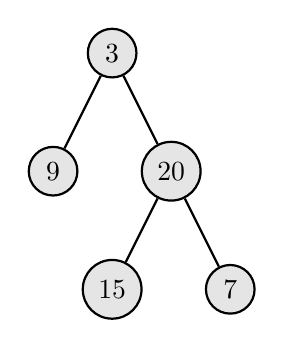
\begin{tikzpicture}
[every node/.style={draw, circle, fill=gray!20!, minimum size=5mm},
thick]
\node{3}
child{node{9}}
child{node{20} child{node{15}} child{node{7}}};
\end{tikzpicture}
\end{figure}



\textbf{Output}:

\fcj{[[9], [3,15], [20], [7]]}
\end{flushleft}
\paragraph{Examples 2:}
\begin{flushleft}
\textbf{Input}: 

\begin{figure}[H]
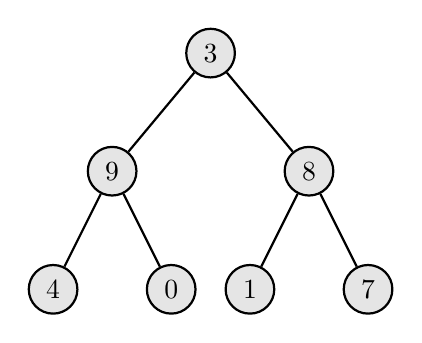
\begin{tikzpicture}
[every node/.style={draw, circle, fill=gray!20!, minimum size=5mm},
level 1/.style={sibling distance=25mm},
level 2/.style={sibling distance=15mm},
thick]
\node{3}
child{node{9} child{node{4}} child{node{0}}}
child{node{8} child{node{1}} child{node{7}}};
\end{tikzpicture}
\end{figure}

\textbf{Output}:

\fcj{[[4], [9], [3,0,1], [8], [7]]}



\end{flushleft}

\subsection{BFS}
Using level traversal, mark each node with a unique number. 

The number of the left child is current node's number minus 1 and the right child is plus 1.

Then we group the nodes with same numbers.


\setcounter{lstlisting}{0}
\begin{lstlisting}[style=customc, caption={BFS}]
vector<vector<int>> verticalOrder( TreeNode* root )
{
    if( !root )
    {
        return {};
    }
    queue<pair<int, TreeNode*>> q;
    q.emplace( 0, root );
    map<int, vector<int>> m;
    while( !q.empty() )
    {
        auto [id, t] = q.front();
        q.pop();
        //add to map
        m[id].push_back( t->val );
        if( t->left )
        {
            q.emplace( id - 1, t->left );
        }
        if( t->right )
        {
            q.emplace( id + 1, t->right );
        }
    }
    //copy data from map to output
    vector<vector<int>> ans;
    for( auto&[id, v] : m )
    {
        ans.emplace_back( begin( v ), end( v ) );
    }
    return ans;
}
\end{lstlisting}

\paragraph{Related Problems}
\begin{itemize}
\item \textbf{102. Binary Tree Level Order Traversal}
\end{itemize}
% \section{315 --- Count of Smaller Numbers After Self}
You are given an integer array $ A $ and you have to return a new counts array $ Z $. The counts array $ Z $ has the property where $ Z[i] $ is the number of smaller elements to the right of $ A[i] $.

\paragraph{Example:}

\begin{flushleft}
\textbf{Input}: $ [5,\;2,\;6,\;1] $
\\
\textbf{Output}: $ [2,\;1,\;1,\;0] $ 
\\
\textbf{Explanation}:
\\
To the right of 5 there are 2 smaller elements (2 and 1).
\\
To the right of 2 there is only 1 smaller element (1).
\\
To the right of 6 there is 1 smaller element (1).
\\
To the right of 1 there is 0 smaller element.
\end{flushleft}
\subsection{Binary Sort}
从$ A[L-1] $即$ A $的最后一个number开始,用leftmost binary search的方法插入到一个新的数组,这样新数组就是有序的,那么此时该数字在新数组中的坐标就是原数组中其右边所有较小数字的个数。之所以用leftmost,是因为要考虑到重复数字的情况。如果用\texttt{STL}的map,计算距离的时间复杂度是$ O(n) $,而用数组的时间复杂度为$ O(1) $。

\setcounter{lstlisting}{0}
\begin{lstlisting}[style=customc, caption={Binary Search And Sorting}]
vector<int> countSmaller( vector<int>& nums )
{
    //process edge scenarios
    if( nums.empty() )
    {
        return {};
    }

    if( nums.size() == 1 )
    {
        return {0};
    }

    vector<int> A; //Sorted nums
    A.reserve( nums.size() );
    A.push_back( nums.back() );

    vector<int> ans( nums.size(), 0 );

    auto L = static_cast< int >( nums.size() );

    for( int i = L - 2; i >= 0; --i )
    {
        int l = 0;
        int curSize = static_cast< int >( A.size() );
        int r = curSize;
        //leftmost binary search
        while( l < r )
        {
            int mid = ( l + r ) / 2;

            if( A[mid] < nums[i] )
            {
                l = mid + 1;
            }
            else
            {
                r = mid;
            }
        }

        ans[i] = l;
        //l is the position in A for nums[i]
        if( l == curSize )
        {
            //nums[i] is the largest, then push back
            A.push_back( nums[i] );
        }
        else
        {
            //otherwise, insert into the correct position
            A.insert( A.begin() + l, nums[i] );
        }
    }
    return ans;
}
\end{lstlisting}

\subsection{Merge Sort}
Merge Sort is suitable for problems which look for some pairs $i$, $j$
such that $i < j$, and $A[i]$, $A[j]$ satisfy some constraints.

We can find such pairs during merge sort. 

In each recursion, before we merge two sorted subarrays, the $i$ is in the left sorted subarray, and the $j$ is in the right sorted subarray. So, we can just go through both sorted subarray to find the valid $i$ and $j$ pairs. As long as this step is $O(n)$, the total time complexity would be $O(n \log n)$.

Such problems do not care about the order of js as long as $j > i$. The $j$ could be possibly anywhere after $i$ as long as $A[j]$ and $A[i]$ satisfy the given constraint. 

Balanced Binary Search Tree would work well for this purpose, but it requires extra code to build the BST and also keep it balanced to avoid $O(N^2)$ worst time complexity. For problems like these, Segment Tree and Binary Indexed Tree are also good choices and give $O(n \log n)$ time complexity.

C++ provides built-ins for merge sort including:

\begin{itemize}
\item \fcj{merge(l1.begin(), l1.end(), l2.begin(), l2.end(), result.begin());} which stores the merged array in \fcj{result}
\item \fcj{inplace_merge(l.begin(), l.middle, l.end())} where array \fcj{[begin, middle)} is merged with array \fcj{[middle, end)}.
\end{itemize}


\begin{lstlisting}[style=customc, caption={Merge Sort}]
vector<int> countSmaller( vector<int>& nums )
{
    if( nums.empty() )
    {
        return {};
    }
    //put value and its index into one array
    vector<pair<int, int>> A( nums.size() );
    int L = ( int )nums.size();
    for( int i = 0; i < L; ++i )
    {
        A[i].first = nums[i];
        A[i].second = i;
    }
    vector<int> ans( nums.size() );
    //do merge sort while getting the answer
    merge_sort( begin( A ), end( A ), ans );
    return ans;
}
void merge_sort( vector<pair<int, int>>::iterator beg, vector<pair<int, int>>::iterator end, vector<int>& ans )
{
    auto dist = distance( beg, end );
    if( dist <= 1 )
    {
        return;
    }

    auto mid = next( beg, dist / 2 );
    merge_sort( beg, mid, ans );
    merge_sort( mid, end, ans );
    //now [beg,mid) and [mid,end) are sorted
    //we then can compare left and right
    for( auto i = beg, j = mid; i != mid; ++i )
    {
        auto [l, l_idx] = ( *i );
        while( j != end )
        {
            auto [r, r_idx] = ( *j );
            if( l > r )
            {
                //smaller numbers in the right hand side
                ++j;
            }
            else
            {
                break;
            }
        }
        ans[l_idx] += ( int )distance( mid, j );
    }
    //do inplace merge
    inplace_merge( beg, mid, end );
}
\end{lstlisting}

\subsection{Binary Index Tree}
We use BIT to store the index of each \fcj{nums[i]} in the sorted array. One way is to make use of a hash map.

\begin{lstlisting}[style=customc, caption={BIT}]
vector<int> countSmaller( vector<int>& nums )
{

    vector<int> A( nums );
    sort( begin( A ), end( A ) );
    int L = ( int )nums.size();
    //use m to record index of each element
    //in the sorted array
    unordered_map<int, int> m;
    for( int i = 0; i < L; ++i )
    {
        m[A[i]] = i + 1;
    }
    //BIT array
    vector<int> BIT( L + 1, 0 );
    for( int i = L - 1; i >= 0; --i )
    {
        //get the index of nums[i]
        //in the sorted array
        int t = m[nums[i]];
        A[i] = query( t - 1, BIT );
        update( t, 1, BIT );
    }
    return A;
}
//get the number of index that
//is larger than index
int query( int index, vector<int>& BIT )
{
    int j = index + 1;
    int res = 0;
    while( j > 0 )
    {
        res += BIT[j];
        j -= ( j & ( -j ) );
    }
    return res;
}
//update index saved in BIT
void update( int index, int diff, vector<int>& BIT )
{
    int j = index + 1;
    int L = ( int )BIT.size();
    while( j < L )
    {
        BIT[j] += diff;
        j += ( j & ( -j ) );
    }
}
\end{lstlisting}

\paragraph{Related Problems}
\begin{itemize}
\item \textbf{327. Count of Range Sum}
\item \textbf{406. Queue Reconstruction by Height}
\item \textbf{493. Reverse Pairs}
\end{itemize}
% \section{316 --- Remove Duplicate Letters}
Given a string which contains only lowercase letters, remove duplicate letters so that every letter appear once and only once. You must make sure your result is the smallest in lexicographical order among all possible results.

\paragraph{Example 1:}

\begin{flushleft}
\textbf{Input}: \texttt{bcabc}
\\
\textbf{Output}: \texttt{abc}
\end{flushleft}

\paragraph{Example 2:}

\begin{flushleft}
\textbf{Input}: \texttt{cbacdcbc}
\\
\textbf{Output}: \texttt{acdb}
\end{flushleft}
\subsection{Hash Map}
这道题其实是要build a monotonically increasing result string.
\par
如果当前letter比result string的last letter小,remove the last letter if the last letter will still appear in the input string later.
\par
算法步骤如下:
\begin{itemize}
\item 建立一个hash map来统计每个字母出现的次数。由于都是lowercase letter,用一个数组$A$即可。
\item 另外,建立一个数组$ x $来纪录每个字母是否被用过,即放入到结果字符串$y$中。
\item 遍历整个字符串,对于遍历到的字符,先在$ A $中decrements其对应的出现次数,然后看$ x $中的值确定其之前是否已经用过,如对应的值为1,即已经在结果字符串中了,因此跳过处理,继续循环。
\item 否则,和当前的存储结果的字符串$y$的last letter进行比较,如果当前letter比$y$的最后一个letter小,并且$y$的last letter的count不为零(即这个letter之后还会出现),那么将$y$的last letter从$ y $中删除,同时将其标记为未用过。
\item 以此类推直至遍历完整个字符串
\end{itemize}
\setcounter{algorithm}{0}
\begin{algorithm}[H]
\caption{Hash Map}
\begin{algorithmic}[1]
\Procedure{RemoveDuplicateLetters}{$S, L$}
\State $\star$ Create an array $A$ to store the counts of each letter in $S$
\State $\star$ Create an array $ x $ to indicate if a letter is contained in the result string
\State $y:=\emptyset$ \Comment The result string
\State $\ast$ Count the frequencies of each letter in $S$
\For{Each $ c $ in $S$}
\State $A[c]\gets A[c] + 1$
\EndFor
\State $\ast$ Process $S$
\For{Each $c$ in $S$}
\State $A[c]\gets A[c]-1$ \Comment Decrements the frequencies of letter $ c $
\If{$x[c]=1$} \Comment letter $ c $ is contained in the result string $ y $
\State \texttt{continue} \Comment Skip to next letter
\EndIf
\While{$y$ is empty \textbf{and} $ y $'s last letter $t$ is larger than $ c $ \textbf{and} $ A[t]>0 $}
\State $\star$ Remove $t$ from $y$
\State $x[t]\gets 0$ \Comment indicate letter $t$ is not contained in the result string $ y $
\EndWhile
\State $y\gets y+c$ \Comment Append $ c $ to $ y $
\State $x[c]\gets 1$ \Comment indicate letter $t$ is contained in the result string $ y $
\EndFor
\State \Return $ y $
\EndProcedure
\end{algorithmic}
\end{algorithm}
\setcounter{lstlisting}{0}
\begin{lstlisting}[style=customc, caption={Hash Map}]
string removeDuplicateLetters( string s )
{
    int L = static_cast<int>( s.size() );
    //indicate if a letter is contained in the result
    vector<int> used( 26, 0 );
    //The frequencies of a letter in s
    vector<int> counts( 26, 0 );
    for( auto c :  s )
    {
        counts[c - 'a'] += 1;
    }
    
    string ans;
    
    for( auto c : s )
    {
        //decrements frequencies of c
        //since we have already visited it
        --counts[c - 'a'];
        //since c is contained in ans,
        //skip to next
        if( used[c - 'a'] )
        {
            continue;
        }

        while( !ans.empty() && ( ans.back() > c ) && ( counts[ans.back() - 'a'] > 0 ) )
        {
            //since ans.back() will be removed
            //indicate it is not contained in ans
            used[ans.back() - 'a'] = 0;
            ans.pop_back();
        }
        //indicate c will be added to ans
        used[c - 'a'] = 1;
        ans.push_back( c );
    }

    return ans;
}
\end{lstlisting}
\section{317 --- Shortest Distance from All Buildings}

\textbf{Hard}

You want to build a house on an empty land which reaches all buildings in the shortest amount of distance. You can only move up, down, left and right. You are given a 2D grid of values 0, 1 or 2, where:

\begin{itemize}
\item Each 0 marks an empty land which you can pass by freely.
\item Each 1 marks a building which you cannot pass through.
\item Each 2 marks an obstacle which you cannot pass through.
\end{itemize}

\paragraph{Example:}

\begin{flushleft}
\textbf{Input}: \fcj{[[1,0,2,0,1],[0,0,0,0,0],[0,0,1,0,0]]}


\textbf{Output}: 7 

\textbf{Explanation}: 

Given three buildings at (0,0), (0,4), (2,2), and an obstacle at (0,2), the point (1,2) is an ideal empty land to build a house, as the total travel distance of $3+3+1=7$ is minimal. So return 7.
\end{flushleft}

\paragraph{Note:}
\begin{itemize}
\item There will be at least one building. 
\item If it is not possible to build such house according to the above rules, return $-1$.
\end{itemize}

\subsection{BFS}
We do BFS starting from each building. Every time, we update the given grid by distance to each building.

To avoid using an array to mark visited cell, we decrement the cell value each time. For example, we search for cell with value of zero and change them to $-1$. Next time, we search for cell with value of $-1$ and change to $-2$. Repeat the same process until all buildings are visited.

\setcounter{lstlisting}{0}
\begin{lstlisting}[style=customc, caption={BFS}]
int shortestDistance( vector<vector<int>>& grid )
{
    int m = ( int )( grid.size() );
    int n = ( int )( grid[0].size() );
    //this sums is used to record
    //distance to each building
    //updated each time for each building
    auto sums( grid );
    //val is used to indicate visited cell
    int val = 0;
    int min_dist = INT_MAX;
    for( int r = 0; r < m; ++r )
    {
        for( int c = 0; c < n; ++c )
        {
            if( grid[r][c] == 1 )
            {
                auto dist( grid );
                min_dist = INT_MAX;
                //start BFS: update distance
                //to this building at (r,c)
                queue<int> q;
                q.push( r * n + c );

                while( !q.empty() )
                {
                    int t = q.front();
                    q.pop();
                    int x = t / n;
                    int y = t - n * x;
                    //update for 4 directions
                    update( x + 1, y, val, dist[x][y], q, grid, dist, sums, min_dist );
                    update( x - 1, y, val, dist[x][y], q, grid, dist, sums, min_dist );
                    update( x, y + 1, val, dist[x][y], q, grid, dist, sums, min_dist );
                    update( x, y - 1, val, dist[x][y], q, grid, dist, sums, min_dist );
                }
                //decrement val
                --val;
            }
        }
    }
    return min_dist == INT_MAX ? -1 : min_dist;
}
//update dist and total dist
void update( int r, int c, int val, int d, queue<int>& q,
             vector<vector<int>>& grid,
             vector<vector<int>>& dist,
             vector<vector<int>>& total,
             int &ans )
{
    int m = ( int )( grid.size() );
    int n = ( int )( grid[0].size() );
    if( ( r >= 0 ) && ( r < m ) && ( c >= 0 ) && ( c < n ) && ( grid[r][c] == val ) )
    {
        //decrements grid[r][c] to mark it as not visited
        grid[r][c] -= 1;
        //update distance to the building
        dist[r][c] = d + 1;
        //accumulate the distance
        total[r][c] += ( dist[r][c] - 1 );
        //update the minimum so far
        ans = ( min )( ans, total[r][c] );
        //add this cell to the queue
        q.push( r * n + c );
    }
}
\end{lstlisting}
% \section{318 --- Maximum Product of Word Lengths}
Given a string array words, find the maximum value of \fcj{length(word[i]) * length(word[j])} where the two words do not share common letters. You may assume that each word will contain only lower case letters. If no such two words exist, return 0.

\paragraph{Example 1:}

\begin{flushleft}
\textbf{Input}: \fcj{["abcw","baz","foo","bar","xtfn","abcdef"]}

\textbf{Output}: 16

\textbf{Explanation}: The two words can be \fcj{"abcw"}, \fcj{"xtfn"}.
\end{flushleft}

\paragraph{Example 2:}

\begin{flushleft}
\textbf{Input}: \fcj{["a","ab","abc","d","cd","bcd","abcd"]}
\\
\textbf{Output}: 4 
\\
\textbf{Explanation}: The two words can be \fcj{"ab"}, \fcj{"cd"}.
\end{flushleft}

\paragraph{Example 3:}

\begin{flushleft}
\textbf{Input}: \fcj{["a","aa","aaa","aaaa"]}

\textbf{Output}: 0 

\textbf{Explanation}: No such pair of words.
\end{flushleft}
\subsection{Bit Mask}
\begin{itemize}
\item 由于只有lowercase letter,因此将每一个字符串可以转换成整数。
\item 一个\texttt{int}有32位,可以用后26位来对应26个字母,若为1,说明该对应位置的字母出现过。
\item 如果两个字符串没有共同的letter,那么这两个字符串对应的整数的AND即为0。
\end{itemize}
\setcounter{lstlisting}{0}
\begin{lstlisting}[style=customc, caption={Bit Mask}]
int maxProduct( vector<string>& words )
{
    vector<int> masks( words.size(), 0 );

    int maxP = 0;

    for( size_t i = 0; i < words.size(); ++i )
    {
        const auto& w = words[i];

        for( auto c : w )
        {
            //using shift to compose an integer
            masks[i] |= ( 1 << ( c - 'a' ) );
        }

        for( size_t j = 0; j < i; ++j )
        {
            if( ( masks[i] & masks[j] ) == 0 )
            {
                //words[i] and words[j] have no common letters
                int P = static_cast< int >( words[i].size() * words[j].size() );
                maxP = ( max )( P, maxP );
            }
        }
    }

    return maxP;
}

\end{lstlisting}
% \section{319 --- Bulb Switcher}
There are $ n $ bulbs that are initially off. You first turn on all the bulbs. Then, you turn off every second bulb. On the third round, you toggle every third bulb (turning on if it's off or turning off if it's on). For the $ i $-th round, you toggle every $ i $ bulb. For the $ n $-th round, you only toggle the last bulb. Find how many bulbs are on after n rounds.

\paragraph{Example:}

\begin{flushleft}
\textbf{Input}: 3

\textbf{Output}: 1 

\textbf{Explanation}: 

At first, the three bulbs are [\texttt{off}, \texttt{off}, \texttt{off}].

After first round, the three bulbs are [\texttt{on}, \texttt{on}, \texttt{on}].

After second round, the three bulbs are [\texttt{on}, \texttt{off}, \texttt{on}].

After third round, the three bulbs are [\texttt{on}, \texttt{off}, \texttt{off}]. 

So you should return 1, because there is only one bulb is on.
\end{flushleft}
\subsection{Mathematic Induction}
\begin{itemize}
\item A bulb最后如果是on的状态,那么它一定是被toggle了奇数次。
\item bulb $ i $ 在 round $ x $如果被toggle了,那么$ i\bmod x = 0 $。因此如果bulb $ i $最后是on的状态,那么它一定有奇数个divisors。
\item Suppose $ i=12 $, 那么它的divisors为$ (1,\;12) $,$ (2,\;6) $,$ (3,\;4) $。很显然对于一般的数来说由于divisor都是成对出现的,因此divisor的数量都是偶数。只有一种情况除外,即square number。在这种情况下,由于某两个divisor是相等的,因此divisor的数量为奇数。
\item 综上所述,最后处于on状态的bulb的编号肯定是平方数。而要计算小于等于$ n $的平方数的个数,直接对$n$开平方取整即可。因为假设$R=\lfloor\sqrt{n}\rfloor$,那么小于$ n $的完全平方数的根就是从1到$ R $,即总共有$R$个。
\end{itemize}
\setcounter{lstlisting}{0}
\begin{lstlisting}[style=customc, caption={Count Of Square Numbers}]
int bulbSwitch( int n )
{
    return sqrt( n );
}
\end{lstlisting}
\section{320 --- Generalized Abbreviation}

\textbf{Medium}

Write a function to generate the generalized abbreviations of a word. 

Note: The order of the output does not matter.

\textbf{Example:}

\begin{flushleft}
\textbf{Input}: \fcj{"word"}

\textbf{Output}:

\begin{lstlisting}[style=customc]
["word", "1ord", "w1rd", "wo1d", "wor1", "2rd", "w2d", "wo2", "1o1d", "1or1", "w1r1", "1o2", "2r1", "3d", "w3", "4"]
\end{lstlisting}
\end{flushleft}

\subsection{Backtracking}

In this problem, the partial candidates in backtracking are incomplete abbreviations that can be extended by one of the two choices:

\begin{enumerate}
\item keep the next character;
\item abbreviate the next character.
\end{enumerate}

\setcounter{lstlisting}{0}
\begin{lstlisting}[style=customc, caption={Backtracking}]
vector<string> generateAbbreviations( string word )
{

    vector<string> ans;
    dfs( word, 0, 0, "", ans );
    return ans;
}
//k: the count of consecutive abbreviated characters
//start: the current index in w
void dfs( string_view w, size_t start, int k, string cur, vector<string>& ans )
{
    if( start == w.size() )
    {
        if( k > 0 )
        {
            //append last k if it is nonzero
            cur += to_string( k );
        }
        ans.emplace_back( cur );
        return;
    }
    //the branch that w[i] is abbreviated
    dfs( w, start + 1, k + 1, cur, ans );
    if( k > 0 )
    {
        cur += to_string( k );
    }
    cur.push_back( w[start] );
    // the branch that w[i] is kept
    // in this case, k is zero
    dfs( w, start + 1, 0, cur, ans );
}
\end{lstlisting}
% \section{321 --- Create Maximum Number}
Given two arrays of length $ m $ and $ n $ with digits 0--9 representing two numbers. Create the maximum number of length $ k \leq m + n $ from digits of the two. The relative order of the digits from the same array must be preserved. Return an array of the k digits.

\paragraph{Note:} 
\begin{itemize}
\item You should try to optimize your time and space complexity.
\end{itemize}

\paragraph{Example 1:}

\begin{flushleft}
\textbf{Input}:
\\
$ A  = [3,\;4,\; 6,\; 5]$
\\
$ B  = [9,\; 1,\; 2, \;5,\; 8,\;3]$
\\
$ k = 5 $
\\
\textbf{Output}: $ [9,\; 8,\; 6,\; 5,\; 3] $
\end{flushleft}

\paragraph{Example 2:}

\begin{flushleft}
\textbf{Input}:
\\
$ A = [6,\; 7] $
\\
$ B = [6,\; 0,\; 4] $
\\
$ k = 5 $
\\
\textbf{Output}: $ [6,\; 7, \;6,\; 0,\; 4] $
\end{flushleft}

\paragraph{Example 3:}

\begin{flushleft}
\textbf{Input}:
\\
$ A = [3,\; 9] $
\\
$ B = [8,\; 9] $
\\
$ k = 3 $
\\
\textbf{Output}: $ [9, \;8, \;9] $
\end{flushleft}
\subsection{Greedy Way}
\begin{enumerate}
\item 首先要确定每个数组中要取几个数,这个只能通过循环一个个测试。比如如果$A$选择取$x$个数,那么$B$就只能选择取$y=k-x$个数
\item For each iteration,对于每个数组,用贪心法得到可能组成的最大数。
\item 然后merge这两个数组得到的最大数,有点类似于merge sort的合并过程。但是需要定义如何进行两个array的比较,这里需要采用lexically comparison的方法。
\item 最后选择所有测试中的最大数。这个过程同样要基于对两个array进行lexically compare的方法。
\item 在对每个数组用贪心的方法取得组成的最大数时,可能最后产生的最大数的长度包含多于给定长度。这是因为在generate的过程中,数组的后面是否还有更大的数,需要不断的放入结果数组中,所以最后需要把多出来的数字去除掉。 \label{step0}
\item 另外在对每个数组用贪心的方法取得组成的最大数的过程中,需要用一个变量来记录该数组中需要drop掉多少个number,即数组长度减去需要的长度。如果没有这个变量来控制,很可能生成的最大数的长度会小于需要的长度。
\end{enumerate}
\setcounter{algorithm}{0}
\begin{algorithm}[H]
\caption{Greedy Way}
\begin{algorithmic}[1]
\Procedure{MaxNumber}{$A, m, B, n, k$}
\State $\ast$ Suppose $x$ is the count of numbers selected from $A$.
\State $\ast$ The minimum for $ x $ is $ \max(k-n, 0) $ and the maximum is $ \min(k, m) $
\State $N:=\emptyset$ \Comment The generated result 
\For{$x:=\max(k-n, 0)$ \textbf{to} $ \min(k, m) $}
\State $ a := $ \Call{Process}{$ A, m, x $} \Comment Generate maximum number array $ a $ from $A$
\State $ b := $ \Call{Process}{$ B, n, k-x $} \Comment Generate maximum number array $ b $ from $B$
\State $ Z:= $ \Call{Merge}{$ a, x, b, k-x $} \Comment Merge $a$ and $b$ based on lexical order
\If{\Call{Compare}{$ N,k,0, Z,k,0 $} is \texttt{true}}
\State $N\gets Z$ \Comment $ N $ is lexically smaller than $ Z $。
\EndIf
\EndFor
\State \Return $N$
\EndProcedure
\end{algorithmic}
\end{algorithm}
Function \texttt{Process} 则是对于任意一个大小为$ L $的输入数组$ T $,generate长度为$ n $的最大数字数组。
\begin{algorithm}[H]
\caption{Generate Maximum Number Array with size $ n $}
\begin{algorithmic}[1]
\Function{Process}{$T, L, n$}
\State $R:=\emptyset$ \Comment The result maximum number array
\State $\delta:=L-n$ \Comment The count of numbers to be dropped from the result maximum number array
\For{Each number $ t $ in $ T $}
\State $\ast$ If $\delta$ is zero, we cannot drop anymore because $R$ needs $n$ digits
\While{$\delta > 0$ \textbf{and} $ R\neq \emptyset $ \textbf{and} $ R[-1] < t $ }
\State $\star$ Drop the last element $R[-1]$ from $R$
\State $\delta\gets\delta-1$
\EndWhile
\State $\star$ Add $n$ to $R$
\EndFor
\State $\star$ Because of drop, $R$ may have more than $n$ digits
\State $\star$ Only keep the first $n$ digits in $R$
\State \Return $ R $
\EndFunction
\end{algorithmic}
\end{algorithm}
Function \texttt{Merge} 则按照lexical order将两个array $ A $和$ B $进行merge,以得到这两个array所能做成的最大number array $M$。
\begin{algorithm}[H]
\caption{Merge two arrays based on lexical order to get maximum number array}
\begin{algorithmic}[1]
\Procedure{Merge}{$A, m, B, n$}
\State $x:=0$ \Comment Index for $A$
\State $y:=0$ \Comment Index for $B$
\State $M:=\emptyset$ \Comment The result string
\State $p:=0$ \Comment Index for $M$
\While{$x<m$ \textbf{or} $ y < n $}
\If{\Call{Compare}{$ A, m, x, B, n, y $} is \texttt{true}}
\State $M[p]:=B[y]$ \Comment $A$ is lexically smaller than $B$, so add $B[y]$ to $M$
\Else
\State $M[p]:=A[x]$ \Comment $A$ is lexically equal or larger than $B$, so add $A[x]$ to $M$
\EndIf
\State $p\gets p+1$ \Comment Move to next slot in $M$
\EndWhile
\algstore{321algo}
\end{algorithmic}
\end{algorithm}
\begin{algorithm}[H]
\begin{algorithmic}[1]
\algrestore{321algo}
\State \Return $M$
\EndProcedure
\end{algorithmic}
\end{algorithm}
最后是Function \texttt{Compare},对两个数组$A$和$B$进行lexically comparison,其中$A$ starts with index $x$ and $ B $ starts with $y$。 如果返回\texttt{true},则表示$A[x\ldots m-1]$ is less than $B[y\ldots n-1]$。
\begin{algorithm}[H]
\caption{Lexically Compare Two Arrays With Different Start Index}
\begin{algorithmic}[1]
\Procedure{Compare}{$A,m,x,B,n,y$}
\While{$x<m$ \textbf{and} $ y<n $}
\If{$A[x] < B[y]$}
\State \Return \texttt{true} \Comment $A$ is smaller than B
\ElsIf{$A[x] > B[x]$}
\State \Return \texttt{false} \Comment $A$ is larger than B
\EndIf
\EndWhile
\State $\star$ 如果算法能到这里,说明 $A[x\ldots m-1]=B[y\ldots n-1]$
\State $\ast$ 需要比较$A$和$B$的长度,
\If{$x=m$ \textbf{and} $ y < n $}
\State \Return \texttt{true} \Comment $A$ is shorter than $B$, so $A[x\ldots m-1]<B[y\ldots n-1]$
\EndIf
\State \Return \texttt{false} \Comment Otherwise, $A[x\ldots m-1]\geq B[y\ldots n-1]$
\EndProcedure
\end{algorithmic}
\end{algorithm}
\setcounter{lstlisting}{0}
\begin{lstlisting}[style=customc, caption={Greedy Approach}]
vector<int> maxNumber( vector<int>& nums1, vector<int>& nums2, int k )
{
    int l1 = static_cast<int>( nums1.size() );
    int l2 = static_cast<int>( nums2.size() );

    //The count of numbers selected from nums1 array
    int sel1 = ( max )( k - l2, 0 );

    //This is the maximum count of numbers
    //can be selected from nums1 array
    int max_sel1 = ( min )( k, l1 );

    vector<int> ans( k, INT_MIN );

    vector<int> merged( k, 0 );

    vector<int> v_maxFrom1;
    vector<int> v_maxFrom2;

    v_maxFrom1.reserve( ( min )( k, l1 ) );
    v_maxFrom2.reserve( ( min )( k, l2 ) );

    for( ; sel1 <= max_sel1; ++sel1 )
    {
        process( nums1, sel1, v_maxFrom1 );
        //k-sel1 is the count of numbers selected from nums2 array
        process( nums2, k - sel1, v_maxFrom2 );

        merge( v_maxFrom1, v_maxFrom2, merged );

        //lexically compare two arrays
        if( lexical_compare( ans, 0, merged, 0 ) )
        {
            swap( ans, merged );
        }

        v_maxFrom1.clear();
        v_maxFrom2.clear();
    }

    return ans;
}

void process( const vector<int>& A, int sel, vector<int>& out )
{
    if( sel == 0 )
    {
        return;
    }

    //drop will control how many numbers
    //will be kept in out array
    int drop = static_cast<int>( A.size() ) - sel;

    for( int n : A )
    {
        while( drop && !out.empty() && ( out.back() < n ) )
        {
            out.pop_back();
            --drop;
        }

        out.push_back( n );
    }


    //since we do not increment drop
    //the final kept numbers will always no less than sel
    out.resize( sel );
}

//Use lexically compare function to compare two arrays
void merge( const vector<int>& v1, const vector<int>& v2, vector<int>& out )
{
    int l1 = static_cast< int >( v1.size() );
    int l2 = static_cast< int >( v2.size() );

    int x = 0;
    int y = 0;

    int p = 0;
    while( ( x < l1 ) || ( y < l2 ) )
    {
        if( lexical_compare( v1, x, v2, y ) )
        {
            out[p] = v2[y];
            ++p;
            ++y;
        }
        else
        {
            out[p] = v1[x];
            ++p;
            ++x;
        }
    }


}

//The routine to compare arrays lexically
bool lexical_compare( const vector<int>& A, int x, const vector<int>& B, int y )
{
    int m = static_cast< int >( A.size() );
    int n = static_cast< int >( B.size() );

    while( ( x < m ) && ( y < n ) )
    {
        if( A[x] < B[y] )
        {
            return true;
        }

        if( A[x] > B[y] )
        {
            return false;
        }

        ++x;
        ++y;
    }

    //A's length is smaller than B's length
    //and all A's numbers equal to previous m numbers in B
    return ( x == m ) && ( y < n );
}
};
\end{lstlisting}
% \section{322 --- Coin Change}
You are given coins of different denominations $C$ and a total amount of money amount $T$. Write a function to compute the fewest number of coins that you need to make up that amount. If that amount of money cannot be made up by any combination of the coins, return $-1$.

\paragraph{Example 1:}

\begin{flushleft}
\textbf{Input}: $C = [1, 2, 5]$,\quad $T = 11$
\\
\textbf{Output}: 3 
\\
\textbf{Explanation}: $ 11 = 5 + 5 + 1 $
\end{flushleft}

\paragraph{Example 2:}

\begin{flushleft}
\textbf{Input}: $C = [2]$, \quad $T = 3$
\\
\textbf{Output}: $ -1 $
\end{flushleft}

\paragraph{Note:}
\begin{itemize}
\item You may assume that you have an infinite number of each kind of coin.
\end{itemize}
\subsection{Kapspack Problem}
典型的kapspack problem,dynamic programming的经典题目。递推公式为

\[
F[i] = \underbrace{\min}_{i \geq C[j]\forall j}(1+F[i-C[j]])
\]
需要建立size为$ 1+T $的递推数组$F$

\setcounter{lstlisting}{0}
\begin{lstlisting}[style=customc, caption={Dynamic Programming}]
int coinChange( vector<int>& coins, int amount )
{
    vector<int> F( amount + 1, amount );

	//initial state
    F[0] = 0;
    
    for( int i = 1; i <= amount; ++i )
    {
        for( int coin : coins )
        {
            if( i >= coin )
            {
                if( F[i - coin] < amount )
                {
                    F[i] = ( min )( F[i], 1 + F[i - coin] );
                }
            }
        }
    }

    return F[amount] == amount ? -1 : F[amount];
}
\end{lstlisting}
% \section{323 --- Number of Connected Components in an Undirected Graph}

\textbf{Medium}

Given $n$ nodes labeled from 0 to $n - 1$ and a list of undirected edges (each edge is a pair of nodes), write a function to find the number of connected components in an undirected graph.

\paragraph{Example 1:}

\begin{flushleft}
\textbf{Input}: $n = 5$ and \fcj{edges = [[0, 1], [1, 2], [3, 4]]}

\textbf{Output}: 2
\end{flushleft}

\paragraph{Example 2:}

\begin{flushleft}
\textbf{Input}: $ n = 5 $ and \fcj{edges = [[0, 1], [1, 2], [2, 3], [3, 4]]}

\textbf{Output}:  1
\end{flushleft}

\paragraph{Note:}
\begin{itemize}
\item You can assume that no duplicate edges will appear in edges. Since all edges are \textbf{undirected}, \fcj{[0, 1]} is the same as \fcj{[1, 0]} and thus will not appear together in \fcj{edges}.
\end{itemize}

\subsection{Union Find}
A typical Union Find problem.

\setcounter{lstlisting}{0}
\begin{lstlisting}[style=customc, caption={Union Find}]
int countComponents( int n, vector<vector<int>>& edges )
{
    vector<int> parents( n, -1 );
    for( int i = 0; i < n; ++i )
    {
        parents[i] = i;
    }
    vector<int> ranks( n, 1 );
    int ans = n;
    for( const auto& edge : edges )
    {
        //get the parent of
        //two vertices of edge
        int px = find( edge[0], parents );
        int py = find( edge[1], parents );
        if( px != py )
        {
            //union them and reduce the
            //number of unconnected parts
            --ans;
            set_union( px, py, parents, ranks );
        }
    }
    return ans;
}
//find parent of x
int find( int x, vector<int>& parents )
{
    while( x != parents[x] )
    {
        x = parents[x];
    }
    return x;
}
//union x and y with path compression
void set_union( int x, int y, vector<int>& parents, vector<int>& ranks )
{
    if( ranks[x] > ranks[y] )
    {
        //make sure x rank is smaller
        swap( x, y );
    }
    else if( ranks[x] == ranks[y] )
    {
        ranks[x]++;
    }
    parents[y] = x;
}
\end{lstlisting}

\paragraph{Related Problems}
\begin{itemize}
\item \textbf{200. Number of Islands}
\item \textbf{261. Graph Valid Tree}
\item \textbf{547. Friend Circles}
\end{itemize}
% \section{324 --- Wiggle Sort II}
Given an unsorted array $ A $, reorder it such that $A[0] < A[1] > A[2] < A[3] \ldots$

\paragraph{Example 1:}

\begin{flushleft}
\textbf{Input}: $A = [1, 5, 1, 1, 6, 4]$
\\
\textbf{Output}: One possible answer is $ [1, 4, 1, 5, 1, 6] $.
\end{flushleft}

\paragraph{Example 2:}

\begin{flushleft}
\textbf{Input}: $A = [1, 3, 2, 2, 3, 1]$
\\
\textbf{Output}: One possible answer is $ [2, 3, 1, 3, 1, 2] $.

\end{flushleft}
\paragraph{Note:}
\begin{itemize}
\item You may assume all input has valid answer.
\end{itemize}

\paragraph{Follow Up:}
\begin{itemize}
\item Can you do it in $ O(n) $ time and/or in-place with $ O(1) $ extra space?
\end{itemize}

\subsection{Sort}
\begin{itemize}
\item Copy原数组到$B$,对B进行排序
\item 从中间将$B$分为两个部分,用两个index,分别指向左右两个部分的最后一个元素
\item 然后遍历原数组,先把左边的最后一个元素放入原数组的第一个位置,然后把右边的最后一个元素放入原数组的第二个位置,接着是左边的倒数第二个元素,然后是右边的倒数第二个元素。依次类推。
\end{itemize}
\setcounter{lstlisting}{0}
\begin{lstlisting}[style=customc, caption={Sort}]
void wiggleSort( vector<int>& nums )
{
    vector<int> A( nums.begin(), nums.end() );

    sort( A.begin(), A.end() );

    int L = static_cast<int>( A.size() );

    //split A into left and right parts
    //at middle
    // A[x] is the last element of right part
    int x = L - 1;
    // A[y] is the last element of left part
    int y = ( L - 1 ) / 2;


    //Put A[y] at A[0], A[2], ...
    //Put A[x] at A[1], A[3], ...
    for( int i = 0; i < L; ++i )
    {
        if( i & 1 )
        {
            nums[i] = A[x];
            --x;
        }
        else
        {
            nums[i] = A[y];
            --y;
        }
    }
}
\end{lstlisting}
\subsection{Partition Based On Median}
\begin{itemize}
\item 首先找到按照median element对$A$进行partition(基于quick select的方法,这种方法的平均复杂度是$ O(n) $),注意,parition后,$A$中numbers的位置都发生了变化,而中间位置的number为$A$的median number。
\item 由于$A$在经过quick select之后,$A(0,\ldots \lfloor (L-1)/2\rfloor)$都是小于median value的number,而$A(\lfloor L/2\rfloor, L-1)$都是大于median value的number,为了能够得到wiggle sort的排列方式,需要将quick select之后$A$中前半段的indcies即$[0\ldots (L-1)/2]$放到$A$中的even indices上,而后半段的indices即$[(L+1)/2\ldots L-1]$放到$A$中的odd indices上。
\par
举例说明,Suppose $ A = [10,11,\ldots 19]$. 经过quick select median value的partition,$A$可能变为
\begin{table}[H]
\begin{tabular}{l*{10}{c}}
index: &  0 &  1 &  2 &  3 &   4 &   5 &  6 &  7 &  8 &   9\\
\hline
$A$[index]:&  11 & 14&  10&  13&   15&   18&  17 & 19&  16&  15
\end{tabular}
\end{table}
其中median为15,目标是将$A$ rearrange为
\begin{table}[H]
\begin{tabular}{l*{10}{c}}
Index: &  0 & 1 & 2 & 3 & 4 & 5 & 6 & 7 & 8 & 9 \\
Mapped: &  5 & 0 & 6 & 1 & 7 & 2 & 8 & 3 & 9 & 4\\
\hline
$A$[index]:&  11 & 18 & 14 & 17 & 10 & 19 & 13 & 16 & 12 & 15
\end{tabular}
\end{table}
其中,大于15的值在quick select后的indicies都在$[5, 9]$中,rearrange后这些数被放入到$A$的奇数indicies中,即$1, 3, 5, \ldots$中。同理,小于15的值在quick select后的indicies都在$[0,3]$中,rearrange后这些数被放入到$A$的偶数indicies中,即$0,2,4,\ldots$中。
\item 一种简单易行的index mapping算法如下

\setcounter{algorithm}{0}
\begin{algorithm}[H]
\caption{Index Mapping Method}
\begin{algorithmic}[1]
\Procedure{M}{$i, n$}
\State $\ast$ We need to find the closest odd number to $n$ which is $n\lor 1$
\State \Return $(2\times i +1)\bmod(n\lor 1)$ 
\EndProcedure
\end{algorithmic}
\end{algorithm}
可以看出,通过这个算法,前半段的index映射为奇数,而后半段的index映射为偶数。例如对于0--9,其对应的mapping index如下所示
\begin{table}[H]
\begin{tabular}{l*{10}{c}}
Original: &  0 & 1 & 2 & 3 & 4 & 5 & 6 & 7 & 8 & 9 \\
Mapped: & 1  &  3 &   5 &   7 &  9 &   0  &  2  &  4 &   6 &   8
\end{tabular}
\end{table}
与之前我们需要rearrange的目标相比,刚好是相反的。
\item 因此为了能够使用上述index mapping算法,采用three-way partition算法。从左到右遍历quick select后的$A$,看当前index的mapping index上$A$的值,由于上述算法和我们的rerarrnage目标相反,所以要将大于median value的swap到前半段indidices的mapping indices上,即那些奇数位置,而小于median value的swap到后半段indices的mapping indices上,即那些偶数位置。所以$A$中三个部分:top, middle 和bottom,top对应大于median value的numbers,middle对应等于median value的numbers,而bottom就是那些小于median value的numbers。
\end{itemize}
\begin{lstlisting}[style=customc, caption={Quick Select And Three-way Partition}]
void wiggleSort( vector<int>& nums )
{
    //quick select to arrange nums by putting
    //median value at center
    nth_element( nums.begin(), nums.begin() + nums.size() / 2, nums.end() );

    //the median value
    int md = nums[nums.size() / 2];

    //index mapping function
    auto getIndex = []( int i, int L )
    {
        return ( 2 * i + 1 ) % ( L );
    };

    int sz = static_cast<int>( nums.size() );
    int oddSz = ( sz | 1 );

    int l = 0; //top part
    int m = 0; //middle part
    int r = sz - 1; //bottom part

    while( m <= r )
    {
        //get mapped index
        int mi = getIndex( m, oddSz );
        if( nums[mi] > md )
        {
            //top part has the numbers
            //that are larger than median value
            //because top part indices are mapped
            //to odd indices
            int li = getIndex( l, oddSz );
            swap( nums[mi], nums[li] );
            ++m;
            ++l;
        }
        else if( nums[mi] < md )
        {
            //bottom part has the numbers
            //that are smaller than median value
            //because bottom part indices are mapped
            //to even indices
            int ri = getIndex( r, oddSz );
            swap( nums[mi], nums[ri] );
            --r;
        }
        else
        {
            ++m;
        }
    }
}

\end{lstlisting}
\subsection{Three Way Parition}
\begin{itemize}
\item 这个算法最开始是解决如下问题的:
\par
The flag of the Netherlands consists of three colors: red, white and blue. Given balls of these three colors arranged randomly in a line (the actual number of balls does not matter), the task is to arrange them such that all balls of the same color are together and their collective color groups are in the correct order.
\item 该算法将一个数组$A$分为三个部分: bottom, middle, and top
\item 在该算法中
\begin{itemize}
\item the top group grow down from the top of the array (即从右到左)
\item the bottom group grow up from the bottom (即从左到右)
\item keep the middle group just above the bottom
\end{itemize}
\item Three-way partition算法保存三个indices,分别是
\begin{enumerate}
\item the index just below the top group
\item the index just above the bottom group, and
\item the index just above the middle.
\end{enumerate}
\item At each step, examine the element just right to the middle.
\begin{enumerate}
\item If it belongs to the top group, swap it with the element just below the top.
\item If it belongs in the bottom, swap it with the element just above the bottom.
\item If it is in the middle, leave it. Update the appropriate index. 
\end{enumerate}
\item Complexity is $ O(n) $ moves and examinations.
\end{itemize}
对应的算法如下,算法中
\begin{itemize}
\item Maintain 3个indices $l$, $ m $ and $ r $。其中$ l\leq m $
\item $r$ holds the boundary of numbers greater than middle $M$.
\item $m$ is the position of number under consideration.
\item $l$ is the boundary for the numbers lesser than the middle $M$.
\end{itemize}
\begin{algorithm}[H]
\caption{Three-way Partition Algorithm}
\begin{algorithmic}[1]
\Procedure{ThreeWayPartition}{$A, L, M$} \Comment M is the middle value
\State $l:=0$
\State $r:=L-1$
\State $m:=0$
\While{$m\leq r$}
\If{$A[m] < M$}
\State $\star$ Swap $A[m]$ and $A[l]$
\State $l\gets l+1$
\State $m\gets m+1$
\ElsIf{$ A[m] > M $}
\State $\star$ Swap $A[m]$ and $A[r]$
\State $r\gets r-1$
\Else
\State $m\gets m+1$
\EndIf
\EndWhile
\EndProcedure
\end{algorithmic}
\end{algorithm}

\paragraph{Related Problems}
\begin{itemize}
\item \textbf{75. Sort Colors}
\item \textbf{215. Kth Largest Element in an Array}
\item \textbf{280. Wiggle Sort}
\end{itemize}

% \section{325 --- Maximum Size Subarray Sum Equals k}

\textbf{Medium}

Given an array \fcj{nums} and a target value $k$, find the maximum length of a subarray that sums to $k$. If there isn't one, return 0 instead.

\paragraph{Note:}

\begin{itemize}
\item The sum of the entire \fcj{nums} array is guaranteed to fit within the 32-bit signed integer range.
\end{itemize}

\paragraph{Example 1:}

\begin{flushleft}
\textbf{Input}: \fcj{nums = [1, -1, 5, -2, 3]}, $ k = 3 $

\textbf{Output}: 4 

\textbf{Explanation}: 

The subarray \fcj{[1, -1, 5, -2]} sums to 3 and is the longest.
\end{flushleft}

\paragraph{Example 2:}

\begin{flushleft}
\textbf{Input}: \fcj{nums = [-2, -1, 2, 1]}, $k = 1$

\textbf{Output}: 2 

\textbf{Explanation}: 

The subarray \fcj{[-1, 2]} sums to 1 and is the longest.

\end{flushleft}

\paragraph{Follow Up:}
\begin{itemize}
\item Can you do it in $O(n)$ time?
\end{itemize}

\subsection{Hash Map}
We make use of a hash map to record the first position of any prefix sum.

\setcounter{lstlisting}{0}
\begin{lstlisting}[style=customc, caption={Hash Map}]
int maxSubArrayLen( vector<int>& nums, int k )
{
    unordered_map<int, int> m;
    int total = 0;
    int L = ( int )nums.size();
    int best = 0;
    for( int i = 0; i < L; ++i )
    {
        total += nums[i];
        if( total == k )
        {
            //this must be the maximum length so far
            best = i + 1;
        }
        else
        {
            //otherwise, we need to find
            //if there were total-k appear before
            auto it = m.find( total - k );
            if( it != m.end() )
            {
                best = ( max )( best, i - it->second );
            }
        }
        //try to emplace into map
        //this will not insert into the map
        //if the key exists
        m.try_emplace( total, i );
    }
    return best;
}
\end{lstlisting}

\paragraph{Related Problems}
\begin{itemize}
\item \textbf{209. Minimum Size Subarray Sum}
\item \textbf{303. Range Sum Query - Immutable}
\item \textbf{525. Contiguous Array}
\item \textbf{713. Subarray Product Less Than K}
\end{itemize}
% \section{326 --- Power of Three}
Given an integer $n$, write a function to determine if it is a power of three.

\paragraph{Example 1:}

\begin{flushleft}
\textbf{Input}: 27
\\
\textbf{Output}: \texttt{true}
\end{flushleft}

\paragraph{Example 2:}

\begin{flushleft}
\textbf{Input}: 0
\\
\textbf{Output}: \texttt{false}
\end{flushleft}

\paragraph{Example 3:}

\begin{flushleft}
\textbf{Input}: 9
\\
\textbf{Output}: \texttt{true}
\end{flushleft}

\paragraph{Example 4:}

\begin{flushleft}
\textbf{Input}: 45
\\
\textbf{Output}: \texttt{false}
\end{flushleft}

\paragraph{Follow up:}
\begin{itemize}
\item Could you do it without using any loop / recursion?
\end{itemize}

\subsection{No Loop}
由于输入是\texttt{int} type,其正整数范围是$0$---$2^{31}$,在此范围中允许的最大的3的次方数为$ 3^{19}=1162261467 $,那么我们只要看这个数能否被$ n $整除即可。
\setcounter{lstlisting}{0}
\begin{lstlisting}[style=customc, caption={No Loop}]
bool isPowerOfThree( int n )
{
    return n > 0 && ( ( 1162261467 % n ) == 0 );
}
\end{lstlisting}
% \section{327 --- Count of Range Sum}
Given an integer array \fcj{nums}, return the number of range sums that lie in \fcj{[lower, upper]} inclusive.

Range \fcj{sum S(i, j)} is defined as the sum of the elements in \fcj{nums} between indices $i$ and $j$ ($i \leq j$), inclusive.

\paragraph{Note:}
\begin{itemize}
\item A naive algorithm of $ O(n^2) $ is trivial. You MUST do better than that.
\end{itemize}

\paragraph{Example:}

\begin{flushleft}
\textbf{Input}: \fcj{nums = [-2,5,-1]}, \fcj{lower = -2}, \fcj{upper = 2},
\\
\textbf{Output}: 3 
\\
\textbf{Explanation}: 

The three ranges are : \fcj{[0,0]}, \fcj{[2,2]}, \fcj{[0,2]} and their respective sums are: $-2$, $-1$, $2$.

\end{flushleft}
\subsection{Prefix Sum}
\begin{itemize}
\item 获得$A$的prefix sum array $Z$。
\item 对于当前的prefix sum $Z[j]$,要找到某个$Z[i]$,使得$l\leq Z[j]-Z[i]\leq u$。即$Z[j]-u\leq Z[i]\leq Z[j]+l$。这个分别通过leftmost and rightmost binary search可以快速定位。
\item 由于prefix sum可能会相同,因此tree map的value是一个array,用来存放对应的index。
\item 最后统计有多少个index满足上述要求。
\item 为了防止数据类型越界,map和prefix sum array的数据类型都用\texttt{long long}。
\end{itemize}
\setcounter{lstlisting}{0}
\begin{lstlisting}[style=customc, caption={Tree Map And Binary Search}]
int countRangeSum( vector<int>& nums, int lower, int upper )
{
    vector<long long> Z( nums.size() + 1, 0 );

    map<long long, vector<int>> m;
    m.emplace( 0, initializer_list<int> {-1} );

    int ans = 0;

    int L = static_cast< int >( nums.size() );

    for( int i = 1; i <= L; ++i )
    {
        Z[i] = Z[i - 1] + nums[i - 1];

        //find the first key in m
        //which is equal or larger than Z[i]- upper
        auto it_low = m.lower_bound( Z[i] - upper );

        if( it_low != m.end() )
        {
            //If this key exists
            //then search for the first key in m
            //which is larger than Z[i]-lower
            auto it_high = m.upper_bound( Z[i] - lower );

            if( it_high != m.begin() )
            {
                //The numbers between *it_low and *it_hight
                //are all candidates. Then accumulate their
                //counts, i.e. the size of the array
                for( auto it = it_low; it != it_high; ++it )
                {
                    ans += static_cast< int >( it->second.size() );
                }
            }
        }

        //Put Z[i] into m
        auto it = m.find( Z[i] );
        if( it == m.end() )
        {
            m.emplace( Z[i], std::initializer_list<int> {i} );
        }
        else
        {
            it->second.push_back( i );
        }
    }

    return ans;
}

//using multiset
int countRangeSum( vector<int>& nums, int lower, int upper )
{
    long long sum = 0;
    multiset<long long> m;
    m.insert( 0 );
    int ans = 0;
    for( int n : nums )
    {
        sum += n;
        //find how many sums
        //such that sum -s <=upper
        //and sum - s > lower;
        //i.e.  sum - upper <= s < sum-lower
        auto hi = m.upper_bound( sum - lower );
        auto lo = m.lower_bound( sum - upper );
        ans += ( int )distance( lo, hi );
        //add sum to m
        m.insert( sum );
    }
    return ans;
}
\end{lstlisting}
\subsection{Merge Sort}
\begin{itemize}
\item 仍然是计算prefix sum。
\item 假设当前的left part和right part都已经sorted。当遍历left part时,对于每个index $i$,需要在right part中找出两个index $k$和$j$,使得
\begin{enumerate}
\item $ Z[j] $ is the first such that $Z[j] - Z[i] > u$
\item $ Z[k] $ is the first such that $ Z[k] - Z[i] \geq l $
\end{enumerate}
这样满足difference为$ [l,u] $之间的区间的个数就是$j-k$。
\item 另外由于这是merge sort,需要另外一个index $\alpha$,用来copy所有满足$Z[\alpha]<Z[i]$的prefix sum到一个cache中以便完成排序的过程。
\item 同样为了避免数据类型越界,prefix sum的类型也是\texttt{long long}。
\end{itemize}
\begin{lstlisting}[style=customc, caption={Merge Sort}]
int countRangeSum( vector<int>& nums, int lower, int upper )
{
    //get prefix sum
    vector<long> sums( nums.size() + 1, 0 );
    for( int i = 0; i < nums.size(); ++i )
    {
        sums[i + 1] = sums[i] + nums[i];
    }
    //call merge sort function
    return countAndMergeSort( sums, 0, sums.size(), lower, upper );
}
int countAndMergeSort( vector<long> &sums, int start, int end, int lower, int upper )
{
    if( end - start <= 1 ) return 0;

    int mid = start + ( end - start ) / 2;
    //split sums into [start,mid-1] and [mid, end]
    int cnt = countAndMergeSort( sums, start, mid, lower, upper ) + countAndMergeSort( sums, mid, end, lower, upper );

    int j = mid, k = mid, t = mid;

    //cache will have the sorted sums elements between start and end
    vector<int> cache( end - start, 0 );

    for( int i = start, r = 0; i < mid; ++i, ++r )
    {
        //find the first sums[k] in right part
        //so that sums[k] - sum[i] >= lower
        while( ( k < end ) && ( sums[k] - sums[i] < lower ) )
        {
            ++k;
        }

        //find the first sums[j] in right part
        //so that sums[j] - sum[i] < upper
        while( ( j < end ) && ( sums[j] - sums[i] <= upper ) )
        {
            ++j;
        }

        //Put all numbers in the right half that less than sums[i]
        //into cache
        while( ( t < end ) && ( sums[t] < sums[i] ) )
        {
            cache[r++] = sums[t++];
        }
        cache[r] = sums[i];

        //The indices between [k,j] are
        //making the range sum fall between [lower, upper]
        cnt += j - k;
    }
    copy( cache.begin(), cache.begin() + t - start, sums.begin() + start );
    return cnt;
}
\end{lstlisting}

We can use STL function \fcc{inplace_merge} to simplify the code

\begin{lstlisting}[style=customc, caption={STL Merge Sort}]
using ll_t = long long;
int countRangeSum( vector<int>& nums, int lower, int upper )
{
    vector<ll_t> psums( nums.size() + 1, 0 );
    for( size_t i = 0; i < nums.size(); ++i )
    {
        psums[i + 1] = nums[i] + psums[i];
    }
    return merge_sort( begin( psums ), end( psums ), lower, upper );
}
//merge sort
int merge_sort( vector<ll_t>::iterator beg, vector<ll_t>::iterator end, int lo, int hi )
{
    auto dist = distance( beg, end );
    if( dist <= 1 )
    {
        return 0;
    }
    auto mid = next( beg, dist / 2 );
    int count = merge_sort( beg, mid, lo, hi ) + merge_sort( mid, end, lo, hi );
    //we need two iterators
    //one records the beginning of number x that x - *i >=lo
    //the other records the beginning of number y that y -*i >=hi
    for( auto i = beg, j1 = mid, j2 = mid; i != mid; ++i )
    {
        while( ( j1 != end ) && ( *j1 - *i < lo ) )
        {
            ++j1;
        }
        while( ( j2 != end ) && ( *j2 - *i <= hi ) )
        {
            ++j2;
        }
        count += ( int )distance( j1, j2 );
    }
    inplace_merge( beg, mid, end );
    return count;
}
\end{lstlisting}


\paragraph{Related Problems}
\begin{itemize}
\item \textbf{315. Count of Smaller Numbers After Self}
\item \textbf{493. Reverse Pairs}
\end{itemize}
% \section{328 --- Odd Even Linked List}
Given a singly linked list $L$, group all odd nodes together followed by the even nodes. Please note here we are talking about the node number and not the value in the nodes.
\par
You should try to do it in place. The program should run in $ O(1) $ space complexity and $ O(N) $ ($ N $ is the number of nodes in $ L $) time complexity.

\paragraph{Example 1:}

\begin{flushleft}
\textbf{Input}: 
\begin{figure}[H]
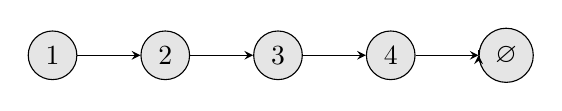
\begin{tikzpicture}
[my/.style={draw, circle, fill=gray!20!, minimum size=5mm}]
\node[my] (1) at (0,0) {1};
\node[my] (2) [right=8mm of 1] {2};
\node[my] (3) [right=8mm of 2] {3};
\node[my] (4) [right=8mm of 3] {4};
\node[my] (5) [right=8mm of 4] {5};
\node[my] (6) [right=8mm of 4] {$\varnothing$};
\draw[>=stealth,->] (1) -- (2);
\draw[>=stealth,->] (2) -- (3);
\draw[>=stealth,->] (3) -- (4);
\draw[>=stealth,->] (4) -- (5);
\draw[>=stealth,->] (5) -- (6);
\end{tikzpicture}
\end{figure}
\textbf{Output}: 
\begin{figure}[H]
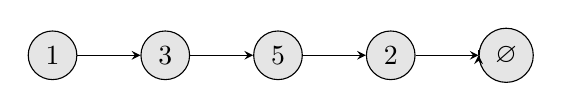
\begin{tikzpicture}
[my/.style={draw, circle, fill=gray!20!, minimum size=5mm}]
\node[my] (1) at (0,0) {1};
\node[my] (2) [right=8mm of 1] {3};
\node[my] (3) [right=8mm of 2] {5};
\node[my] (4) [right=8mm of 3] {2};
\node[my] (5) [right=8mm of 4] {4};
\node[my] (6) [right=8mm of 4] {$\varnothing$};
\draw[>=stealth,->] (1) -- (2);
\draw[>=stealth,->] (2) -- (3);
\draw[>=stealth,->] (3) -- (4);
\draw[>=stealth,->] (4) -- (5);
\draw[>=stealth,->] (5) -- (6);
\end{tikzpicture}
\end{figure}

\end{flushleft}
\paragraph{Example 2:}
\begin{flushleft}
\textbf{Input}: 
\begin{figure}[H]
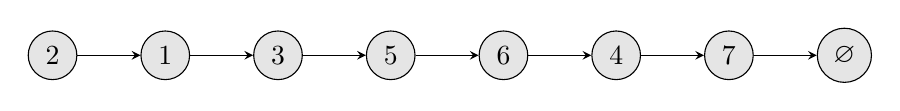
\begin{tikzpicture}
[my/.style={draw, circle, fill=gray!20!, minimum size=5mm}]
\node[my] (1) at (0,0) {2};
\node[my] (2) [right=8mm of 1] {1};
\node[my] (3) [right=8mm of 2] {3};
\node[my] (4) [right=8mm of 3] {5};
\node[my] (5) [right=8mm of 4] {6};
\node[my] (6) [right=8mm of 5] {4};
\node[my] (7) [right=8mm of 6] {7};
\node[my] (8) [right=8mm of 7] {$\varnothing$};
\draw[>=stealth,->] (1) -- (2);
\draw[>=stealth,->] (2) -- (3);
\draw[>=stealth,->] (3) -- (4);
\draw[>=stealth,->] (4) -- (5);
\draw[>=stealth,->] (5) -- (6);
\draw[>=stealth,->] (6) -- (7);
\draw[>=stealth,->] (7) -- (8);
\end{tikzpicture}
\end{figure}
\textbf{Output}: 
\begin{figure}[H]
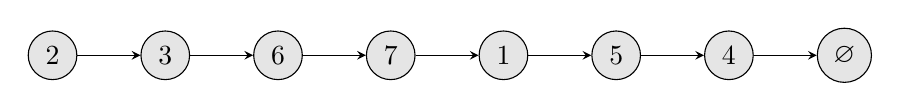
\begin{tikzpicture}
[my/.style={draw, circle, fill=gray!20!, minimum size=5mm}]
\node[my] (1) at (0,0) {2};
\node[my] (2) [right=8mm of 1] {3};
\node[my] (3) [right=8mm of 2] {6};
\node[my] (4) [right=8mm of 3] {7};
\node[my] (5) [right=8mm of 4] {1};
\node[my] (6) [right=8mm of 5] {5};
\node[my] (7) [right=8mm of 6] {4};
\node[my] (8) [right=8mm of 7] {$\varnothing$};
\draw[>=stealth,->] (1) -- (2);
\draw[>=stealth,->] (2) -- (3);
\draw[>=stealth,->] (3) -- (4);
\draw[>=stealth,->] (4) -- (5);
\draw[>=stealth,->] (5) -- (6);
\draw[>=stealth,->] (6) -- (7);
\draw[>=stealth,->] (7) -- (8);
\end{tikzpicture}
\end{figure}
\end{flushleft}

\paragraph{Note:}

\begin{itemize}
\item The relative order inside both the even and odd groups should remain as it was in the input.
\item The first node is considered odd, the second node even and so on \dots
\end{itemize}

\subsection{Two Pointers}
\begin{itemize}
\item 建立两个指针,分别指向odd和even节点,同时记录even节点的头。
\item 遍历链表时,先把odd节点的next指向even的next,然后odd前进到其next节点。
\item 接着把even节点的next指向当前odd的next,由于odd已经更新为even的下一个节点,因此odd的next节点就是下一个even节点。
\item 然后even前进到其next节点。以此类推
\item 最后把odd节点的next设置为开始时保存的even节点的头。
\end{itemize}

\setcounter{lstlisting}{0}
\begin{lstlisting}[style=customc, caption={Two Pointers}]
ListNode* oddEvenList( ListNode* head )
{
    if( !head )
    {
        return head;
    }

    auto odd = head;
    auto even = head->next;

    auto evenHead = even;

    while( even && even->next )
    {
        odd->next = even->next;
        odd = odd->next;
        even->next = odd->next;
        even = even->next;
    }

    odd->next = evenHead;
    return head;
}
\end{lstlisting}

\paragraph{Related Problems}
\begin{itemize}
\item \textbf{725. Split Linked List in Parts}
\end{itemize}
% \section{329 --- Longest Increasing Path in a Matrix}
Given an integer matrix $M$, find the length of the longest increasing path.
\par
From each cell, you can either move to four directions: left, right, up or down. You may \textbf{NOT} move diagonally or move outside of the boundary (i.e. wrap-around is not allowed).

\paragraph{Example 1:}

\begin{flushleft}
\textbf{Input}: 
\begin{table}[H]
\begin{tabular}{ccc}
\textcolor{red}{9} & 9 & 4 \\
\textcolor{red}{6} &6 & 8\\
\textcolor{red}{2}& \textcolor{red}{1} & 1
\end{tabular}
\end{table}
\textbf{Output}: 4
\\ 
\textbf{Explanation}: The longest increasing path is $[1,\; 2,\; 6,\; 9]$.
\end{flushleft}

\paragraph{Example 2:}

\begin{flushleft}
\textbf{Input}: 
\begin{table}[H]
\begin{tabular}{ccc}
\textcolor{red}{3} & \textcolor{red}{4} & \textcolor{red}{5} \\
3 &2 & \textcolor{red}{6}\\
2& 2 & 1
\end{tabular}
\end{table}
\textbf{Output}: 4 
\\
\textbf{Explanation}: The longest increasing path is $ [3,\; 4, \;5, \;6] $. Moving diagonally is not allowed.
\end{flushleft}
\subsection{Dynamic Programming + DFS}
\begin{itemize}
\item 由于每个cell其实都存在一个以这个cell为开始的longest increasing path,因此用一个memo数组来记录这个path的length。
\item 对每一个cell进行DFS搜索,直至出界或者下一个cell小于等于当前cell的值。
\end{itemize}
\setcounter{lstlisting}{0}
\begin{lstlisting}[style=customc, caption={Dynamic Programming + DFS}]
int longestIncreasingPath( vector<vector<int>>& matrix )
{
    if( matrix.empty() || matrix[0].empty() )
    {
        return 0;
    }

    int m = static_cast<int>( matrix.size() );
    int n = static_cast<int>( matrix[0].size() );

    vector<vector<int>> memo( m, vector<int>( n, 0 ) );

    int best = 1;

    for( int r = 0; r < m; ++r )
    {
        for( int c = 0; c < n; ++c )
        {
            //test each cell
            int len = dfs( matrix, r, c, m, n memo );
            best = ( max )( best, len );
        }
    }

    return best;
}

int dfs( vector<vector<int>>& matrix, int r, int c, int rows, int cols, vector<vector<int>>& memo )
{
    //if we already get the maximum length
    //starting from this cell
    //just return
    if( memo[r][c] )
    {
        return memo[r][c];
    }

    int dr[] = {-1, 0, 1, 0};
    int dc[] = {0, -1, 0, 1};

    int best = 1;

    for( int i = 0; i < 4; ++i )
    {
        int nr = r + dr[i];
        int nc = c + dc[i];

        if( ( nr < 0 ) || ( nr >= rows ) || ( nc < 0 ) || ( nc >= cols ) || ( matrix[nr][nc] <= matrix[r][c] ) )
        {
            //out of bound or
            //next cell is no larger than current cell
            continue;
        }

        int len = 1 + dfs( matrix, nr, nc, memo );
        best = ( max )( best, len );
    }

    memo[r][c] = best;
    return best;
}
\end{lstlisting}


% \section{330 --- Patching Array}
Given a sorted positive integer array $A$ and an integer $ n $, add/patch elements to the array such that any number in range $ [1, n] $ inclusive can be formed by the sum of some elements in the array. Return the minimum number of patches required.

\paragraph{Example 1:}

\begin{flushleft}
\textbf{Input}: $A = [1,3]$, $n = 6$
\\
\textbf{Output}: 1 
\\
\textbf{Explanation}:
\\
Combinations of $A$ are $[1]$, $[3]$, $ [1,3] $, which form possible sums of: 1, 3, 4.
\\
Now if we add/patch 2 to $ A $, the combinations are: $ [1] $, $ [2] $, $ [3] $, $ [1,3] $, $ [2,3] $, $ [1,2,3] $.
\\
Possible sums are 1, 2, 3, 4, 5, 6, which now covers the range $ [1, 6] $.
\\
So we only need 1 patch.
\end{flushleft}

\paragraph{Example 2:}

\begin{flushleft}
\textbf{Input}: $ A = [1,5,10] $, $ n = 20 $
\\
\textbf{Output}: 2
\\
\textbf{Explanation}: The two patches can be $ [2, 4] $.
\end{flushleft}

\paragraph{Example 3:}

\begin{flushleft}
\textbf{Input}: $A = [1,2,2]$, $n = 5$
\\
\textbf{Output}: 0
\end{flushleft}
\subsection{Dynamic Programming}
\begin{enumerate}
\item 定义一个变量$ x $,用来表示目前数组$A$加上已经有的patch number不能够build出的最小值,即当前build出的range为$[0\ldots x-1]$。
\item 初始化为$x$为1。
\item 由于能得到的数字范围是$[0, x-1]$,如果在$A$中有number $y\leq x$,那么我们可以把build的范围扩大到$[0\ldots x-1+y]$。
\item 而如果$y>x$,那么此时就需要添加一个patch number。这个number需要选择为能最大限度的增加能够得到的range。很显然这个数就是$x$。
\item 按照上述过程遍历完整个数组,即可得到结果所要求的patch number。
\end{enumerate}
例如,假设输入数组$A = [1, 5, 10] $, $ n=20 $。
\begin{itemize}
\item 初始化$x$为1。即最开始能够得到range为$[0]$。
\item 由于$A$中第一个数1小等于$x$,因此直接加上这个数扩展range。这时候range扩展为$[0, 1]$,$x$更新为2。
\item $A$下一个数5对于2来说比较大,因此要加上一个patch number $x$即2,扩展range到$[0, 3]$,$x$更新为4。
\item 接下来5仍然大于$x$,因此继续加上一个patch number 4,扩展range到$[0,8]$,$x$更新为9。
\item 由于这时候5小于$x$,加上这个数继续扩展range,这时候range扩展为$[0, 14]$,$x$更新为15。
\item  $A$再下一个数10小于15,加上这个扩展range为$[0, 25]$。已经能够覆盖$[0,20]$了。
\end{itemize}

\setcounter{algorithm}{0}
\begin{algorithm}[H]
\caption{Dynamic Programming}
\begin{algorithmic}[1]
\Procedure{MinPatches}{$A, L, n$}
\State $x:=1$ \Comment We have built range $ [0\ldots x-1] $
\State $\alpha:=0$ \Comment The number of patches
\State $i:=0$ \Comment The index in $A$
\While{$ x \leq  n $}
\If{$i<L$ \textbf{and} $ A[i] \leq x $}
\State $x\gets x+A[i]$ \Comment Extend the range to $[0\ldots x-1+A[i]]$
\State $i\gets i+1$
\Else
\State $x\gets x$ \Comment Add a patch number $x$ to extend range to $[0\ldots x-1+x]$
\State $\alpha\gets \alpha+1$ \Comment Increments the number of patches
\EndIf
\EndWhile
\State \Return $\alpha$
\EndProcedure
\end{algorithmic}
\end{algorithm}

\setcounter{lstlisting}{0}
\begin{lstlisting}[style=customc, caption={Dynamic Programming}]
int minPatches( vector<int>& nums, int n )
{
    //expand to long long type
    //to avoid data type overflow
    long long x = 1;
    auto ll_n = static_cast<int>( n );

    size_t i = 0;
    int ans = 0;

    while( x <= ll_n )
    {
        if( ( i < nums.size() ) && ( nums[i] <= x ) )
        {
            //extend the range to [0,x-1+nums[i]]
            x += nums[i];
            ++i;
        }
        else
        {
            //add a patch number x
            //extend the range to [0, x-1+x]
            x += x;
            ++ans;
        }
    }

    return ans;
}

\end{lstlisting}


% \section{331 --- Verify Preorder Serialization of a Binary Tree}
One way to serialize a binary tree is to use pre-order traversal. When we encounter a non-null node, we record the node's value. If it is a null node, we record using a sentinel value such as $\star$.
\begin{figure}[H]
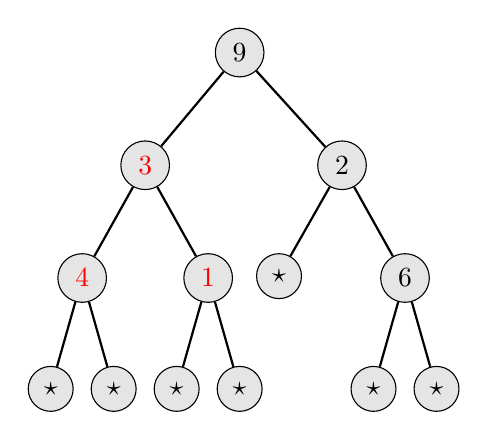
\begin{tikzpicture}
[my/.style={draw, circle, fill=gray!20!, minimum size=5mm}]
\node[my](1) at (0,0) {9};
\node[my](2)[below=8mm of 1, xshift=-12mm] {\textcolor{red}{3}};
\node[my](3)[below=8mm of 1, xshift=13mm] {2};
\node[my](4)[below=8mm of 2, xshift=-8mm] {\textcolor{red}{4}};
\node[my](5)[below=8mm of 2, xshift=8mm] {\textcolor{red}{1}};
\node[my](6)[below=8mm of 3, xshift=-8mm] {$\star$};
\node[my](7)[below=8mm of 3, xshift=8mm] {6};
\node[my](8)[below=8mm of 4, xshift=-4mm] {$\star$};
\node[my](9)[below=8mm of 4, xshift=4mm] {$\star$};
\node[my](10)[below=8mm of 5, xshift=-4mm] {$\star$};
\node[my](11)[below=8mm of 5, xshift=4mm] {$\star$};
\node[my](12)[below=8mm of 7, xshift=-4mm] {$\star$};
\node[my](13)[below=8mm of 7, xshift=4mm] {$\star$};
\draw[thick] (1) -- (2);
\draw[thick] (1) -- (3);
\draw[thick] (2) -- (4);
\draw[thick] (2) -- (5);
\draw[thick] (3) -- (6);
\draw[thick] (3) -- (7);
\draw[thick] (4) -- (8);
\draw[thick] (4) -- (9);
\draw[thick] (5) -- (10);
\draw[thick] (5) -- (11);
\draw[thick] (7) -- (12);
\draw[thick] (7) -- (13);
\end{tikzpicture}
\end{figure}
For example, the above binary tree can be serialized to the string $9,3,4,\star,\star,1,\star,\star,2,\star,6,\star,\star$, where $\star$ represents a null node.
\par
Given a string of comma separated values, verify whether it is a correct preorder traversal serialization of a binary tree. Find an algorithm without reconstructing the tree.
\par
Each comma separated value in the string must be either an integer or a character $\star$ representing null pointer.
\par
You may assume that the input format is always valid, for example it could never contain two consecutive commas such as $1,,3$.

\paragraph{Example 1:}
\begin{flushleft}
\textbf{Input}: \fcj{"9,3,4,#,#,1,#,#,2,#,6,#,#"}

\textbf{Output}: \fcc{true}
\end{flushleft}

\paragraph{Example 2:}
\begin{flushleft}
\textbf{Input}: \fcj{"1,#"}

\textbf{Output}: \fcc{false}
\end{flushleft}

\paragraph{Example 3:}
\begin{flushleft}
\textbf{Input}: \fcj{"9,#,#,1"}

\textbf{Output}: \fcc{false}
\end{flushleft}

\subsection{Iteration}
Binary tree could be considered as a number of slots to fulfill. 

At the start there is just one slot available for a number or null node. Both number and null node take one slot to be placed. 

For the \fcj{null} node the story ends up here, whereas the number will add into the tree two slots for the child nodes. Each child node could be, again, a number or a \fcj{null}.

The idea is straightforward : take the nodes one by one from \textit{preorder} traversal, and compute the number of available slots. If at the end all available slots are used up, the \textit{preorder} traversal represents the valid serialization.

\setcounter{lstlisting}{0}
\begin{lstlisting}[style=customc, caption={Iteration}]
bool isValidSerialization( string preorder )
{
    // number of available slots
    int slots = 1;
    for( size_t i = 0; i < preorder.size(); ++i )
    {
        if( preorder[i] == ',' )
        {
            // one node takes one slot
            --slots;
            // no more slots available
            if( slots < 0 )
            {
                return false;
            }
            // non-empty node creates two children slots
            if( ( i > 0 ) && ( preorder[i - 1] != '#' ) )
            {
                slots += 2;
            }
        }
    }
    //for the last node
    //since there is no comma, we only add or subtract one
    if( preorder.back() == '#' )
    {
        slots -= 1;
    }
    else
    {
        ++slots;
    }
    return slots == 0;
}
\end{lstlisting}
% \section{332 --- Reconstruct Itinerary}
Given a list of airline tickets represented by pairs of departure and arrival airports \fcj{[from, to]}, reconstruct the itinerary in order. All of the tickets belong to a man who departs from JFK. Thus, the itinerary must begin with JFK.

\paragraph{Note:}
\begin{itemize}
\item  there are multiple valid itineraries, you should return the itinerary that has the smallest lexical order when read as a single string. For example, the itinerary \fcj{["JFK", "LGA"]} has a smaller lexical order than \fcj{["JFK", "LGB"]}.
\item All airports are represented by three capital letters (IATA code).
\item You may assume all tickets form at least one valid itinerary.
\end{itemize}

\paragraph{Example 1:}

\begin{flushleft}
\textbf{Input}:  \fcj{[["MUC", "LHR"], ["JFK", "MUC"], ["SFO", "SJC"], ["LHR", "SFO"]]}
\\
\textbf{Output}: \fcj{["JFK", "MUC", "LHR", "SFO", "SJC"]}

\end{flushleft}

\paragraph{Example 2:}

\begin{flushleft}
\textbf{Input}: \fcj{[["JFK","SFO"],["JFK","ATL"],["SFO","ATL"],["ATL","JFK"],["ATL","SFO"]]}

\textbf{Output}: \fcj{["JFK","ATL","JFK","SFO","ATL","SFO"]}
\\
\textbf{Explanation}: 

Another possible reconstruction is: \fcj{["JFK","SFO","ATL","JFK","ATL","SFO"]}. But it is larger in lexical order.
\end{flushleft}
\subsection{Depth First Search}
\begin{itemize}
\item 首先建立邻接表,用一个hash map,key为出发的城市string,value则为该出发城市的目的地集合。因为题目要求按字母顺序的,同时考虑到重复情况,实际实现的时候用\texttt{multiset}。
\item 接着从\texttt{JFK}开始\texttt{DFS},如果当前string对应的目的地集合不为空,将目的地集合中的第一个节点也是当前字母顺序最小的目的地取出来,并将其在集合中删掉,然后继续递归遍历这个节点。
\item 当该出发城市的目的地集合变为空了,表示我们已经递归遍历了其所有目的地,这时候将该出发城市代码string加入到结果中。
\item 注意,结果中的顺序其实是相反的,最后返回的时候reverse得到的结果。
\end{itemize}
\setcounter{lstlisting}{0}
\begin{lstlisting}[style=customc, caption={Depth First Search}]
vector<string> findItinerary( vector<pair<string, string>> tickets )
{
    unordered_map<string, multiset<string>> g;

    //create adjacent list
    for( const auto& p : tickets )
    {
        auto it = g.find( p.first );

        if( it == g.end() )
        {
            g.emplace( p.first, initializer_list<string> {p.second} );
        }
        else
        {
            it->second.emplace( p.second );
        }
    }

    vector<string> ans;
    dfs( g, "JFK", ans );

    //Reverse ans to get final result
    return {ans.rbegin(), ans.rend()};
}

void dfs( unordered_map<string, multiset<string>>& g, string start, vector<string>& ans )
{
    while( !g[start].empty() )
    {
        //iterate over all destinations for start
        auto it = g[start].begin();
        string next = *it;
        //remove the first one from the destinations
        g[start].erase( it );

        //continue DSF on this destination
        dfs( g, next, ans );

    }

    //Finally, we have processed all destinations
    //Add the start to the answer
    ans.emplace_back( start );

}
\end{lstlisting}
\subsection{Stack Based Iterative Way}
\begin{itemize}
\item 同样是建立邻近表图。
\item 用一个栈而不是队列来进行。因为我们需要将所有的目的地访问完,才能回到出发点。
\item 开始时将\texttt{JFK}入栈
\item 然后每次从检查栈顶元素,看于其相连的节点,即目的地集合是否为空,如果为空,则将该元素加入结果中,并将栈顶元素弹出。否则从相连的节点中取出第一个即当前字母顺序最小的那个目的地,放入栈中,同时从相连的节点set中删除该节点。
\item 注意我们不能每次就弹出栈顶元素,因为目的地集合还没有empty的情况下,我们仍旧需要访问该栈顶元素。
\item 最后返回的时候还是需要reverse得到的结果。
\end{itemize}
\begin{lstlisting}[style=customc, caption={Stack}]
vector<string> findItinerary( vector<pair<string, string>> tickets )
{
    unordered_map<string, multiset<string>> g;

    //create adjacent list
    for( const auto& p : tickets )
    {
        auto it = g.find( p.first );

        if( it == g.end() )
        {
            g.emplace( p.first, initializer_list<string> {p.second} );
        }
        else
        {
            it->second.emplace( p.second );
        }
    }

    stack<string> stk;
    stk.emplace( "JFK" );

    vector<string> ans;
    while( !stk.empty() )
    {
        auto t = stk.top();
        if( g[t].empty() )
        {
            //add t to ans
            ans.emplace_back( t );
            //we only pop t at there
            stk.pop();
        }
        else
        {
            //get the first destinatino
            //from t's adjacent list
            auto next = *( g[t].begin() );
            stk.emplace( next );
            //remove this destination from
            //t's adjacent list
            g[t].erase( g[t].begin() );
        }
    }

    //Reverse ans to get the result
    return {ans.rbegin(), ans.rend()};
}

\end{lstlisting}


% \section{333 --- Largest BST Subtree}
Given a binary tree, find the largest subtree which is a Binary Search Tree (BST), where largest means subtree with largest number of nodes in it.
\paragraph{Note:}
\begin{itemize}
    \item A subtree must include all of its descendants. 
\end{itemize}
\par
Here's an example:
\begin{figure}[H]
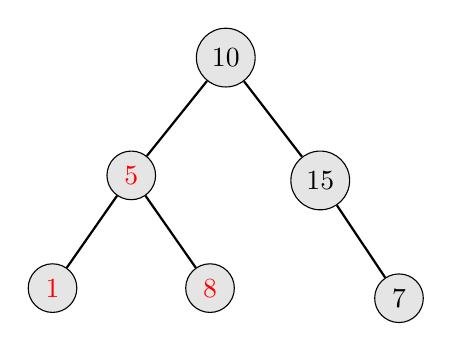
\begin{tikzpicture}
[my/.style={draw, circle, fill=gray!20!, minimum size=5mm}]
\node[my](1) at (0,0) {10};
\node[my](2)[below=8mm of 1, xshift=-12mm] {\textcolor{red}{5}};
\node[my](3)[below=8mm of 1, xshift=12mm] {15};
\node[my](4)[below=8mm of 2, xshift=-10mm] {\textcolor{red}{1}};
\node[my](5)[below=8mm of 2, xshift=10mm] {\textcolor{red}{8}};
\node[my](6)[below=8mm of 3, xshift=10mm] {7};
\draw[thick] (1) -- (2);
\draw[thick] (1) -- (3);
\draw[thick] (2) -- (4);
\draw[thick] (2) -- (5);
\draw[thick] (3) -- (6);
\end{tikzpicture}
\end{figure}
The Largest BST Subtree in this case is the highlighted one. 
\par
The return value is the subtree's size, which is 3.

\paragraph{Hint:}
\begin{itemize}
    \item You can recursively use algorithm similar to 98. Validate Binary Search Tree at each node of the tree, which will result in $O(n\log n)$ time complexity.
\end{itemize}

\paragraph{Follow up:}
\begin{itemize}
    \item Can you figure out ways to solve it with $O(n)$ time complexity?
\end{itemize}
% \section{334 --- Increasing Triplet Subsequence}
Given an unsorted array return whether an increasing subsequence of length 3 exists or not in the array.
\par
Formally the function should:
\begin{itemize}
\item Return \texttt{true} if there exists \texttt{i}, \texttt{j}, \texttt{k} such that $A[i] < A[j] < [k]$ given $0 \leq i < j < k \leq n-1$ else return \texttt{false}.

\end{itemize}

\paragraph{Note:} 
\begin{itemize}
\item Your algorithm should run in $O(n)$ time complexity and $O(1)$ space complexity.
\end{itemize}

\paragraph{Example 1:}

\begin{flushleft}
\textbf{Input}: $[1,2,3,4,5]$
\\
\textbf{Output}: \fcc{true}
\end{flushleft}

\paragraph{Example 2:}

\begin{flushleft}
\textbf{Input}: $[5,4,3,2,1]$
\\
\textbf{Output}: \fcc{false}
\end{flushleft}



\subsection{Find The Minimum Two Numbers}
\begin{itemize}
\item 算法类似于寻找最小数和次最小数
\item 设定两个变量$ x $和$ y $,初始化都设为int type的最大值。
\item 遍历数组$A$,对于当前数字$ n $
\begin{itemize}
\item 如果 $ x\geq n $,将$ x $更新为$n$. 
\item 否则,如果$ y\geq n $,则将$ y $更新为$n$
\item 如果$y$被更新,说明之前$x$比当前这个$y$还小,这样就找到了两个数是递增关系。
\item 最后如果$x<n$, $y<n$,因为$x<y$,我们就找到了符合要求的三个数。
\end{itemize}
\end{itemize}
\setcounter{lstlisting}{0}
\begin{lstlisting}[style=customc, caption={Find Minimum}]
bool increasingTriplet( vector<int>& nums )
{
    //The minimum
    int x = INT_MAX;
    //The one larger than minimum
    int y = INT_MAX;

    for( int n : nums )
    {
        if( n <= x )
        {
            x = n;
        }
        else if( n <= y )
        {
            //If we update y
            //x <y
            y = n;
        }
        else
        {
            //x<n, y<n and x <y
            //Found the 3 numbers
            return true;
        }
    }

    //No such 3 numbers exist
    return false;
}
\end{lstlisting}

\paragraph{Related Problems}
\begin{itemize}
\item \textbf{300. Longest Increasing Subsequence}
\end{itemize}


% \section{335 --- Self Crossing}
You are given an array $ x $ of $ n $ positive numbers. You start at point $ (0,0) $ and moves $ x[0] $ metres to the north, then $ x[1] $ metres to the west, $ x[2] $ metres to the south, $ x[3] $ metres to the east and so on. In other words, after each move your direction changes counter-clockwise.
\par
Write a one-pass algorithm with $ O(1) $ extra space to determine, if your path crosses itself, or not.

 

\paragraph{Example 1:}

\begin{flushleft}
\begin{figure}[H]
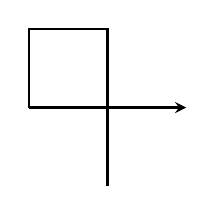
\begin{tikzpicture}
\draw[thick] (0,0) -- ++(0,2) -- ++(-1,0) -- ++(0,-1); 
\draw[thick,>=stealth,->] (-1,1) -- (1,1);
\end{tikzpicture}
\end{figure}
\textbf{Input}: $ [2,1,1,2] $
\\
\textbf{Output}: \texttt{true}
\end{flushleft}

\paragraph{Example 2:}

\begin{flushleft}
\begin{figure}[H]
\begin{tikzpicture}
\draw[thick] (0,0) -- ++(0,1) -- ++(-2,0) -- ++(0,-3) -- ++(4,0);
\draw[thick,>=stealth,->] (-2,-2) -- (2,-2);
\end{tikzpicture}
\end{figure}
\textbf{Input}: [1,2,3,4]
\\
\textbf{Output}: \texttt{false} 
\end{flushleft}

\paragraph{Example 3:}

\begin{flushleft}
\begin{figure}[H]
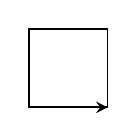
\begin{tikzpicture}
\draw[line width=0.7pt] (0,0) -- ++(0,1) -- ++(-1,0) -- ++(0,-1) -- ++(1,0);
\draw[thick,>=stealth,->] (-1,0) -- (0,0);
\end{tikzpicture}
\end{figure}
\textbf{Input}: $ [1,1,1,1] $
\\
\textbf{Output}: \texttt{true} 
\end{flushleft}

\subsection{Analysis}
实际上相交的情况只有以下三种情况
\begin{enumerate}
\item 第四条边和第一条边相交的情况,需要满足的条件是第一条边大于等于第三条边 ($ x_0\geq x_2 $),第四条边大于等于第二条边 ($ x_3 \geq x_1 $)。同样适用于第五条边和第二条边相交,第六条边和第三条边相交等等,依次向后类推的情况
\begin{figure}[H]
\begin{tikzpicture}
\draw[thick] (0,0) -- ++(0,4) -- ++(-2,0) -- ++(0,-2); 
\draw[thick,>=stealth,->] (-2,2) -- (2,2);
\node (0) at (0.5,3) {{\small $x_0$}};
\node (0) at (-1,4.5) {{\small $x_1$}};
\node (0) at (-2.5,3) {{\small $x_2$}};
\node (0) at (-0.5,2.4) {{\small $x_3$}};
\end{tikzpicture}
\caption{Case 1: $ x_0\geq x_2 $, $ x_3\geq x_1 $}
\end{figure}
\item 第二类是第五条边和第一条边重合相交的情况,需要满足的条件是第二条边和第四条边相等 ($ x_1=x_3 $),第五条边大于等于第三条边和第一条边的差值 ($ x_4\geq x_2 - x_0 $),同样适用于第六条边和第二条边重合相交的情况等等依次向后类推。
\begin{figure}[H]
\begin{tikzpicture}
\draw[thick, color=blue] (0,0) -- ++(0,2) -- ++(-3,0) -- ++(0,-4) -- ++(3,0);
\draw[thick, >=stealth,->, color=red] (0,-2) -- (0,0);
\node at (0.5,1) {{\small $x_0$}};
\node at (-1.5,2.5) {{\small $x_1$}};
\node at (-3.5,0) {{\small $x_2$}};
\node at (-1.5,-2.5) {{\small $x_3$}};
\node at (0.5,-1) {{\small $x_4$}};
\end{tikzpicture}
\caption{Case 2: $ x_1=x_3 $, $ x_4\geq x_2 - x_0 $ }
\end{figure}
\item 第三类是第六条边和第一条边相交的情况,需要满足的条件是第四条边大于等于第二条边($ x_3 \geq x_1 $),第三条边大于等于第五条边 ($ x_2 \geq x_4 $),第五条边大于等于第三条边和第一条边的差值 ($ x4 \geq x_2 - x_0 $),第六条边大于等于第四条边和第二条边的差值 ($ x_5\geq x_3-x_1 $),同样适用于第七条边和第二条边相交的情况等等依次向后类推。
\begin{figure}[H]
\begin{tikzpicture}
\draw[thick, color=blue] (0,0) -- ++(0,3) -- ++(-3,0) -- ++(0,-5) -- ++(5,0) -- ++(0,3);
\draw[thick, >=stealth,->, color=red] (2,1) -- (-1,1);
\node at (0.5,2.3) {{\small $x_0$}};
\node at (-1.5,3.5) {{\small $x_1$}};
\node at (-3.5,0.5) {{\small $x_2$}};
\node at (-0.5,-2.5) {{\small $x_3$}};
\node at (2.5,-0.5) {{\small $x_4$}};
\node at (1,0.5) {{\small $x_5$}};
\end{tikzpicture}
\caption{Case 3: $ x_3\geq x_1 $, $ x_2\geq x_4 $, $ x_4\geq x_2 - x_0 $, $x_5\geq x_3-x_1$}
\end{figure}
\end{enumerate}
\setcounter{algorithm}{0}
\begin{algorithm}[H]
\caption{Three Cases}
\begin{algorithmic}[1]
\Procedure{IsSelfCrossing}{$x, L$}
\For{$i:=3$ \textbf{to} $L-1$}
\State $\ast$ Case 1
\State $x_0 = x[i-3]$, $ x_1= x[i-2] $, $ x_2 = x[i-1] $, $ x_3 = x[i] $
\If{$ x_0 \geq x_2 $ \textbf{and} $ x_3\geq x_1 $}
\State \Return \texttt{true}
\EndIf
\If{$i\geq 4$}
\State $\ast$ Case 2
\State $x_0 = x[i-4]$, $ x_1= x[i-3] $, $ x_2 = x[i-2] $, $ x_3 = x[i-1] $, $ x_4 = x[i] $
\If{$x_1=x_3$ \textbf{and} $ x_4\geq x_2-x_0 $}
\State \Return \texttt{true}
\EndIf
\EndIf
\If{$i\geq 5$}
\State $\ast$ Case 3
\State $x_0 = x[i-5]$, $ x_1= x[i-4] $, $ x_2 = x[i-3] $, $ x_3 = x[i-2] $, $ x_4 = x[i-1] $, $ x_5 = x[i] $
\If{$x_3\geq x_1$ \textbf{and} $ x_2\geq x_4 $ \textbf{and} $ x_4\geq x_2-x_0 $ \textbf{and} $ x_5\geq x_3 -x_1 $}
\State \Return \texttt{true}
\EndIf
\algstore{335algo}
\end{algorithmic}
\end{algorithm}
\begin{algorithm}[H]
\begin{algorithmic}[1]
\algrestore{335algo}
\EndIf
\EndFor
\EndProcedure
\end{algorithmic}
\end{algorithm}
\setcounter{lstlisting}{0}
\begin{lstlisting}[style=customc, caption={Three Cases}]
bool isSelfCrossing( vector<int>& x )
{
    int y[6] = {0};

    for( size_t i = 3; i < x.size(); ++i )
    {
        y[0] = x[i - 3];
        y[1] = x[i - 2];
        y[2] = x[i - 1];
        y[3] = x[i];

        //case 1:
        if( ( y[0] >= y[2] ) && ( y[3] >= y[1] ) )
        {
            return true;
        }

        //case 2:
        if( i >= 4 )
        {
            y[0] = x[i - 4];
            y[1] = x[i - 3];
            y[2] = x[i - 2];
            y[3] = x[i - 1];
            y[4] = x[i];

            if( ( y[3] == y[1] ) && ( y[4] >= y[2] - y[0] ) )
            {
                return true;
            }

        }

        //case 3:
        if( i >= 5 )
        {
            y[0] = x[i - 5];
            y[1] = x[i - 4];
            y[2] = x[i - 3];
            y[3] = x[i - 2];
            y[4] = x[i - 1];
            y[5] = x[i];

            if( ( y[3] >= y[1] ) && ( y[2] >= y[4] ) && ( y[4] >= y[2] - y[0] ) && ( y[5] >= y[3] - y[1] ) )
            {
                return true;
            }
        }

    }

    return false;
}

\end{lstlisting}
% \section{336 --- Palindrome Pairs}
Given a list of \textbf{unique} words, find all pairs of distinct indices $ (i, j) $ in the given list, so that the concatenation of the two words, i.e. \fcj{words[i] + words[j]} is a palindrome.

\paragraph{Example 1:}

\begin{flushleft}
\textbf{Input}:\fcj{["abcd","dcba","lls","s","sssll"]}

\textbf{Output}: \fcj{[[0,1],[1,0],[3,2],[2,4]]}  

\textbf{Explanation}: The palindromes are \fcj{["dcbaabcd","abcddcba","slls","llssssll"]}
\end{flushleft}

\paragraph{Example 2:}

\begin{flushleft}
\textbf{Input}: \fcj{["bat","tab","cat"]}

\textbf{Output}: \fcj{[[0,1],[1,0]]} 

\textbf{Explanation}:The palindromes are \fcj{["battab","tabbat"]}
\end{flushleft}

\subsection{Hash Map}
Maintain a hash map which has map between each reversed word and its index.

Then, iterate original array, and for each word, split into left and right part at each index. Check if any part is a palindrome, and if another part can be found in the hash map.



\setcounter{lstlisting}{0}
\begin{lstlisting}[style=customc, caption={Hash Map}]
vector<vector<int>> palindromePairs( vector<string>& words )
{
    unordered_map<string_view, int> m;
    //to make hash map has string_view key
    //we need another array to store the reversed word
    vector<string> rev_words( words );
    int wi = 0;
    //empties save the index of word which is empty
    vector<int> empties;
    for( auto& word : rev_words )
    {
        if( word.empty() )
        {
            empties.push_back( wi++ );
            continue;
        }
        reverse( begin( word ), end( word ) );
        m.emplace( word, wi++ );
    }
    wi = 0;
    vector<vector<int>> ans;
    //helper function to check if a string s is a palindrome
    auto is_palindrome = []( string_view s )
    {
        return equal( begin( s ), begin( s ) + s.size() / 2, rbegin( s ) );
    };
    for( const auto& word : words )
    {
        auto it = m.find( word );
        if( ( it != m.end() ) && ( it->second != wi ) )
        {
            //found a pair
            ans.emplace_back( vector<int> {wi, it->second} );
        }
        //if word is palindrome and there are empty words
        //any pair of them is also a palindrome
        if( is_palindrome( word ) && !empties.empty() )
        {
            for( int j : empties )
            {
                if( j != wi )
                {
                    ans.emplace_back( vector<int> {wi, j} );
                    ans.emplace_back( vector<int> {j, wi} );
                }
            }
        }
        //check substr at each part
        string_view w = word;
        for( size_t i = 1; i < w.size(); ++i )
        {
            auto left = w.substr( 0, i );
            auto right = w.substr( i );
            it = m.find( left );
            if( ( it != m.end() ) && is_palindrome( right ) && ( it->second != wi ) )
            {
                //wi + wi[0,i] is a palindrome
                ans.emplace_back( vector<int> {wi, it->second} );
            }
            it = m.find( right );
            if( ( it != m.end() ) && is_palindrome( left ) && ( it->second != wi ) )
            {
                //wi[i,..] + wi is a palindrome
                ans.emplace_back( vector<int> {it->second, wi} );
            }
        }
        ++wi;
    }
    return ans;
}
\end{lstlisting}

\paragraph{Related Problems}
\begin{itemize}
\item \textbf{5. Longest Palindromic Substring}
\item \textbf{214. Shortest Palindrome}
\end{itemize}



% \section{337 --- House Robber III}

\textbf{Medium}

The thief has found himself a new place for his thievery again. There is only one entrance to this area, called the \textit{root}. Besides the root, each house has one and only one parent house. After a tour, the smart thief realized that \textit{all houses in this place forms a binary tree}. It will automatically contact the police if two directly-linked houses were broken into on the same night.

Determine the maximum amount of money the thief can rob tonight without alerting the police.

\paragraph{Example 1:}
\begin{flushleft}


\textbf{Input}: \fcj{[3,2,3,null,3,null,1]}

\begin{figure}[H]
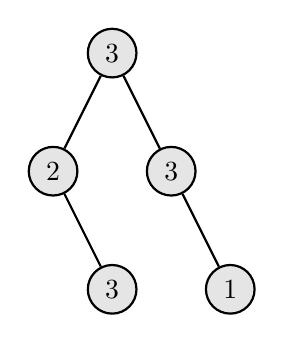
\begin{tikzpicture}
[every node/.style={draw, circle, fill=gray!20!, minimum size=5mm},
%level 1/.style={sibling distance=25mm},
%level 2/.style={sibling distance=15mm},
thick]
\node{3}
child{node{2} child[missing] child{node{3}}}
child{node{3} child[missing] child{node{1}}};
\end{tikzpicture}
\end{figure}

\textbf{Output}: 7
 
\textbf{Explanation}: Maximum amount of money the thief can rob is $3 + 3 + 1 = 7$.
\end{flushleft}

\paragraph{Example 2:}
\begin{flushleft}


\textbf{Input}: \fcj{[3,4,5,1,3,null,1]}

\begin{figure}[H]
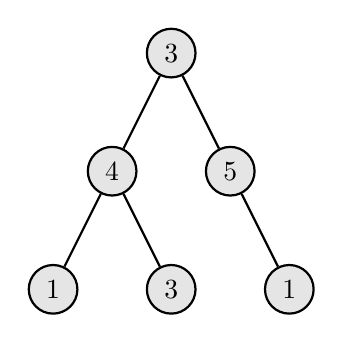
\begin{tikzpicture}
[every node/.style={draw, circle, fill=gray!20!, minimum size=5mm},
%level 1/.style={sibling distance=25mm},
%level 2/.style={sibling distance=15mm},
thick]
\node{3}
child{node{4} child{node{1}} child{node{3}}}
child{node{5} child[missing] child{node{1}}};
\end{tikzpicture}
\end{figure}

\textbf{Output}: 9

\textbf{Explanation}: Maximum amount of money the thief can rob is $4 + 5 = 9$.

\end{flushleft}

\setcounter{lstlisting}{0}
\begin{lstlisting}[style=customc, caption={DFS}]
int rob( TreeNode* root )
{
    unordered_map<TreeNode*, int> memo;
    return dfs( root, memo );
}
int dfs( TreeNode* t, unordered_map<TreeNode*, int>& memo )
{
    if( !t )
    {
        return 0;
    }
    auto it = memo.find( t );
    if( it != memo.end() )
    {
        return it->second;
    }
    //first find the value of rob t
    int val = 0;
    if( t->left )
    {
        val += dfs( t->left->left, m ) + dfs( t->left->right, m );
    }

    if( t->right )
    {
        val += dfs( t->right->left, m ) + dfs( t->right->right, m );
    }
    //now find the value of not robbing t
    int rob_without_t = dfs( t->left, m ) + dfs( t->right, m );
    val = ( max )( val + root->val, rob_without_t );
    memo.emplace( t, val );
    return val;
}
\end{lstlisting}
% \section{338 --- Counting Bits}

\textbf{Medium}

Given a non negative integer number $n$. For every numbers $i$ in the range $0 \leq i \leq n$ calculate the number of 1's in their binary representation and return them as an array.

\paragraph{Example 1:}

\begin{flushleft}
\textbf{Input}: 2

\textbf{Output}: \fcj{[0,1,1]}
\end{flushleft}

\paragraph{Example 2:}

\begin{flushleft}
\textbf{Input}: 5

\textbf{Output}: \fcj{[0,1,1,2,1,2]}
\end{flushleft}

\paragraph{Follow up:}

\begin{itemize}
\item It is very easy to come up with a solution with run time \fcj{O(n*sizeof(int))}. But can you do it in linear time $O(n)$ /possibly in a single pass?
\item Space complexity should be $O(n)$.
\item Can you do it like a boss? Do it without using any builtin function like\fcc{ __builtin_popcount} in \fcc{c++} or in any other language.
\end{itemize}

\subsection{Dynamic Programming}

Suppose we have an integer:
\[
x = (1001011101)_2 = (605)_{10}
\]

and we already calculated and stored all the results of 0 to $x - 1$.

Then we know that $x$ is differ by rightmost bit with a number we already calculated:

\[
\hat{x} = (1001011100)_2 = (604)_{10}
\]

\setcounter{lstlisting}{0}
\begin{lstlisting}[style=customc, caption={DP}]
vector<int> countBits( int num )
{
    vector<int> F( num + 1, 0 );
    for( int i = 1; i <= num; ++i )
    {
        //find the number that is differ with
        //i by rightmost bit 1
        F[i] = F[i & ( i - 1 )] + 1;
    }
    return F;
}
\end{lstlisting}


\section{339 --- Nested List Weight Sum}

\textbf{Easy}

Given a nested list of integers, return the sum of all integers in the list weighted by their depth.

Each element is either an integer, or a list -- whose elements may also be integers or other lists.

\paragraph{Example 1:}

\begin{flushleft}
\textbf{Input}: \fcj{[[1,1],2,[1,1]]}

\textbf{Output}: 10 

\textbf{Explanation}: Four 1's at depth 2, one 2 at depth 1.
\end{flushleft}

\paragraph{Example 2:}

\begin{flushleft}
\textbf{Input}: \fcj{[1,[4,[6]]]}

\textbf{Output}: 27 

\textbf{Explanation}: 

One 1 at depth 1, one 4 at depth 2, and one 6 at depth 3; $1 + 4\times 2 + 6\times 3 = 27$.
\end{flushleft}

\subsection{DFS}
Because the input is nested, it is natural to think about the problem in a recursive way. 

We go through the list of nested integers one by one, keeping track of the current depth $d$. 

If a nested integer is an integer $n$, we calculate its sum as $n\times d$. 

If the nested integer is a list, we calculate the sum of this list recursively using the same process but with depth $d+1$.

\setcounter{lstlisting}{0}
\begin{lstlisting}[style=customc, caption={DFS}]
int depthSum( vector<NestedInteger>& nestedList )
{
    int sum = 0;
    for( const auto& ni : nestedList )
    {
        sum += dfs( ni, 1 );
    }
    return sum;
}
//get the sum recurisvely with level
int dfs( const NestedInteger& ni, int level )
{
    if( ni.isInteger() )
    {
        return ni.getInteger() * level;
    }
    //for list, recurisvely get the sum
    int sum = 0;
    for( const auto& child : ni.getList() )
    {
        sum += dfs( child, level + 1 );
    }
    return sum;
}
\end{lstlisting}

\subsection{BFS}
This problem can also be solved using BFS with level traverse

\begin{lstlisting}[style=customc, caption={BFS}]
int depthSum( vector<NestedInteger>& nestedList )
{
    //using reference_wrapper to avoid copy object
    queue<reference_wrapper<const NestedInteger>> q;
    int ans = 0;
    for( const auto& ni : nestedList )
    {
        q.push( cref( ni ) );
        int level = 1;
        while( !q.empty() )
        {
            auto sz = q.size();
            for( size_t i = 0; i < sz; ++i )
            {
                auto e = q.front();
                q.pop();
                if( e.get().isInteger() )
                {
                    ans += e.get().getInteger() * level;
                }
                else
                {
                    //if it is not integer
                    //push into the queue
                    for( const auto& next : e.get().getList() )
                    {
                        q.push( cref( next ) );
                    }
                }
            }
            ++level;
        }
    }
    return ans;
}
\end{lstlisting}

\paragraph{Related Problems}
\begin{itemize}
\item \textbf{364. Nested List Weight Sum II}
\item \textbf{565. Array Nesting}
\item \textbf{690. Employee Importance}
\end{itemize}
% \section{340 --- Longest Substring with At Most K Distinct Characters}

\textbf{Hard}

Given a string, find the length of the longest substring T that contains at most $k$ distinct characters.

\paragraph{Example 1:}

\begin{flushleft}
\textbf{Input}: \fcj{s = "eceba"}, $k = 2$

\textbf{Output}: 3

Explanation: T is \fcj{"ece"} which its length is 3.
\end{flushleft}

\paragraph{Example 2:}

\begin{flushleft}
\textbf{Input}: \fcj{s = "aa"}, $k = 1$

\textbf{Output}: 2

\textbf{Explanation}: T is \fcj{"aa"} which its length is 2.
\end{flushleft}

\subsection{Sliding Window}
The idea is to set both pointers in the position 0 and then move right pointer to the right while the window contains not more than $k$ distinct characters. 

If at some point we've got $k + 1$ distinct characters, we move left pointer to keep not more than $k + 1$ distinct characters in the window.

When the input string contains $n$ distinct characters, at each step one uses $O(k)$ time to find a minimum value in the hashmap with $k$ elements and so the overall time complexity is $O(Nk)$.

\setcounter{lstlisting}{0}
\begin{lstlisting}[style=customc, caption={Sliding Window With Hash Map}]
int lengthOfLongestSubstringKDistinct( string s, int k )
{
    if( s.empty() || ( k == 0 ) )
    {
        return 0;
    }
    size_t left = 0;
    unordered_map<char, int> fly;
    int ans = 0;
    for( size_t right = 0; right < s.size(); ++right )
    {
        fly[s[right]] += 1;
        int sz = ( int )fly.size();
        while( ( left < right ) && ( sz > k ) )
        {
            //shrink the window to make sure
            //no larger than k distinct letters
            //are there
            auto it = fly.find( s[left] );
            if( it->second == 1 )
            {
                //s[left] is completely removed
                //so erase it from fly
                fly.erase( s[left] );
            }
            else
            {
                --it->second;
            }
            sz = ( int )fly.size();
            ++left;
        }
        ans = ( max )( ans, ( int )right - ( int )left + 1 );
    }
    return ans;
}
\end{lstlisting}


\section{341 --- Flatten Nested List Iterator}

\textbf{Medium}

Given a nested list of integers, implement an iterator to flatten it.

Each element is either an integer, or a list -- whose elements may also be integers or other lists.

\paragraph{Example 1:}

\begin{flushleft}
\textbf{Input}: \fcj{[[1,1],2,[1,1]]}

\textbf{Output}: \fcj{[1,1,2,1,1]}

\textbf{Explanation}: 

By calling next repeatedly until \fcj{hasNext} returns \fcc{false}, the order of elements returned by next should be: \fcj{[1,1,2,1,1]}.
\end{flushleft}

\paragraph{Example 2:}

\begin{flushleft}
\textbf{Input}: \fcj{[1,[4,[6]]]}

\textbf{Output}: \fcj{[1,4,6]}

\textbf{Explanation}: 

By calling next repeatedly until \fcj{hasNext} returns \fcc{false}, the order of elements returned by next should be: \fcj{[1,4,6]}.

\end{flushleft}

\subsection{Stack}
Use a stack to save the result of unpacking each NestedInteger until a integer appear

\setcounter{lstlisting}{0}
\begin{lstlisting}[style=customc, caption={Stack}]
/**
 * // This is the interface that allows for creating nested lists.
 * // You should not implement it, or speculate about its implementation
 * class NestedInteger {
 *   public:
 *     // Return true if this NestedInteger holds a single integer, rather than a nested list.
 *     bool isInteger() const;
 *
 *     // Return the single integer that this NestedInteger holds, if it holds a single integer
 *     // The result is undefined if this NestedInteger holds a nested list
 *     int getInteger() const;
 *
 *     // Return the nested list that this NestedInteger holds, if it holds a nested list
 *     // The result is undefined if this NestedInteger holds a single integer
 *     const vector<NestedInteger> &getList() const;
 * };
 */
class NestedIterator
{
public:
    NestedIterator( vector<NestedInteger> &nestedList )
    {
        //add all NestedInteger into the stack from end to begin
        for( auto it = nestedList.rbegin(); it != nestedList.rend(); ++it )
        {
            stk.push( it );
        }
    }
    int next()
    {
        //get integer from top of stack
        auto t = stk.top();
        stk.pop();
        return t->getInteger();
    }

    bool hasNext()
    {
        while( !stk.empty() )
        {
            auto t = stk.top();
            if( t->isInteger() )
            {
                //this is integer
                return true;
            }
            stk.pop();
            //unpack the non integer list
            auto& l = t->getList();
            for( auto it = rbegin( l ); it != rend( l ); ++it )
            {
                stk.push( it );
            }
        }
        return false;
    }
    //we need reverse_iterator type
    using IterT = vector<NestedInteger>::reverse_iterator;
    stack<IterT> stk;
};
/**
 * Your NestedIterator object will be instantiated and called as such:
 * NestedIterator i(nestedList);
 * while (i.hasNext()) cout << i.next();
 */
\end{lstlisting}

\paragraph{Related Problems}
\begin{itemize}
\item \textbf{251. Flatten 2D Vector}
\item \textbf{281. Zigzag Iterator}
\item \textbf{385. Mini Parser}
\item \textbf{565. Array Nesting}
\end{itemize}
% \section{342 --- Power of Four}

\textbf{Easy}

Given an integer (signed 32 bits), write a function to check whether it is a power of 4.

\paragraph{Example 1:}

\begin{flushleft}
\textbf{Input}: 16

\textbf{Output}: \fcc{true}
\end{flushleft}

\paragraph{Example 2:}

\begin{flushleft}
\textbf{Input}: 5

\textbf{Output}: \fcc{false}
\end{flushleft}

\paragraph{Follow up:}
\begin{itemize}
\item Could you solve it without loops/recursion?
\end{itemize}

\subsection{Bit Operation}
We know how to check if a number is a power of 2.

Now the problem is to distinguish between even powers of two (when $x$ is a power of four) and odd powers of two (when $x$ is not a power of four). 

In binary representation both cases are single 1-bit followed by zeros.

What is the difference? In the first case (power of four), 1-bit is at even position: bit 0, bit 2, bit 4, etc. In the second case, at odd position.

Hence power of four would make a zero in a bitwise AND with number $(101010\ldots 10)_2$

How long should be $(101010\ldots 10)_2$ if $x$ is a signed integer? Answer is 32 bits. 

It's common to use hexadecimal representation: $(101010\ldots 10)_2 = (aaaaaaaa)_{16}$

\setcounter{lstlisting}{0}
\begin{lstlisting}[style=customc, caption={Bit Operation}]
bool isPowerOfFour( int num )
{
    if( ( num > 0 ) && ( ( num & ( num - 1 ) ) == 0 ) )
    {
        //num is power of 2
        //check if it is even power of 2
        return ( num & 0xaaaaaaaa ) == 0;
    }
    return false;
}
\end{lstlisting}

\paragraph{Related Problems}
\begin{itemize}
\item \textbf{231. Power of Two}
\item \textbf{326. Power of Three}
\end{itemize}
% \section{343 --- Integer Break}
Given a positive integer $ n $, break it into the sum of at least two positive integers and maximize the product of those integers. Return the maximum product you can get.

\paragraph{Example 1:}

\begin{flushleft}
\textbf{Input}: 2
\\
\textbf{Output}: 1
\\
\textbf{Explanation}: $2 = 1 + 1$, $1 \times 1 = 1$.
\end{flushleft}

\paragraph{Example 2:}

\begin{flushleft}
\textbf{Input}: 10
\\
\textbf{Output}: 36
\\
\textbf{Explanation}: $10 = 3 + 3 + 4$, $3 \times 3 \times 4 = 36$.
\end{flushleft}

\paragraph{Note:} 
\begin{itemize}
\item You may assume that $ n $ is not less than 2 and not larger than 58.
\end{itemize}

\subsection{Dynamic Programming}
假设$ F(n) $为整数$n$分解后能得到的最大product,我们需要从1到$ n-1 $逐个进行分解测试,如果当前测试的数为$ i $,这时候$ n $ 分解成 $ i $和$ n-i $两个数字,那么有两种情况

\begin{enumerate}
\item $ n-i $不再进行分解,这时候的product为$i \times (n-i)$
\item $n-i$ 继续分解,所能得到的最大product为 $ F(n-i) $, 而$ n $能得到的product为 $ i\times F[n-i] $
\item 取这两者的最大值与当前$ F(n) $进行比较,将$ F(n) $ update为较大值。
\end{enumerate}

\setcounter{lstlisting}{0}
\begin{lstlisting}[style=customc, caption={Dynamic Programming}]
int integerBreak( int n )
{
    vector<int> F( n + 1, 1 );

    for( int i = 3; i <= n; ++i )
    {
        for( int j = 1; j < i; ++j )
        {
            F[i] = ( max )( F[i], ( i - j ) * j ); // (i-j) is one number
            F[i] = ( max )( F[i], j * F[i - j] ); // dissecting (i-j)
        }
    }

    return F[n];
}

\end{lstlisting}
% \section{344 --- Reverse String}
Write a function that reverses a string. The input string is given as an array of characters $A$.
\par
Do not allocate extra space for another array, you must do this by modifying the input array in-place with $O(1)$ extra memory.
\par
You may assume all the characters consist of printable \texttt{ascii} characters.

 

\paragraph{Example 1:}

\begin{flushleft}
\textbf{Input}: [h,\quad e,\quad l,\quad l,\quad o]
\\
\textbf{Output}: [o,\quad l,\quad l,\quad e,\quad h]
\end{flushleft}

\paragraph{Example 2:}

\begin{flushleft}
\textbf{Input}: [H,\quad a,\quad n,\quad n,\quad a,\quad h]
\\
\textbf{Output}: [h,\quad a,\quad n,\quad n,\quad a,\quad H]
\end{flushleft}

\subsection{In-place Swap}
Too easy problem

\setcounter{lstlisting}{0}
\begin{lstlisting}[style=customc, caption={In-place Swap}]
void reverseString( vector<char>& s )
{
    int l  = 0;
    int r = static_cast<int>( s.size() ) - 1;

    while( l < r )
    {
        swap( s[l], s[r] );
        ++l;
        --r;
    }
}
\end{lstlisting}
% \section{345. Reverse Vowels of a String}
Write a function that takes a string $S$ as input and reverse only the vowels of a string.

\paragraph{Example 1:}

\begin{flushleft}
\textbf{Input}: \texttt{hello}
\\
\textbf{Output}: \texttt{holle}
\end{flushleft}


\paragraph{Example 2:}

\begin{flushleft}
\textbf{Input}: \texttt{leetcode}
\\
\textbf{Output}: \texttt{leotcede}
\end{flushleft}

\paragraph{Note:}
\begin{itemize}
\item The vowels does not include the letter $y$.
\end{itemize}

\subsection{Two Pointers}
\begin{itemize}
\item Use two indexes $l$ and $r$ to point to the beginning and end of $S$
\item Inside the loop, loop until the next vowel
\item Whenever $l\geq r$, jump out of the loop and return the updated string $S$
\end{itemize}

\setcounter{lstlisting}{0}
\begin{lstlisting}[style=customc, caption={Two Pointers}]
string reverseVowels( string s )
{
    int l = 0;
    int r = static_cast<int>( s.size() ) - 1;

    unordered_set<char> vowels{'a', 'A', 'e', 'E', 'i', 'I', 'o', 'O', 'u', 'U'};

    while( l < r )
    {
        while( ( l < r ) && ( vowels.find( s[l] ) == vowels.end() ) )
        {
            ++l;
            continue;
        }

        while( ( l < r ) && ( vowels.find( s[r] ) == vowels.end() ) )
        {
            --r;
            continue;
        }

        if( l >= r )
        {
            //no longer to search
            return s;
        }

        swap( s[l], s[r] );
        ++l;
        --r;
    }

    return s;
}

\end{lstlisting}

We can also make use of STL function \fcc{find_first_of} and \fcc{find_last_of} to solve. 

In \fcc{find_first_of}, there is a parameter \fcc{pos}, which means the search only happens in \fcc{s[pos, s.size())}.

For \fcc{find_last_of}, the parameter \fcc{pos}, which means the search only happens in \fcc{s[0, pos]}

\begin{lstlisting}[style=customc, caption={STL}]
string reverseVowels( string s )
{
    size_t left = 0;
    size_t right = s.size() - 1;
    string vowels = "aeiouAEIOU";
    while( left < right )
    {
        //search in [left, size())
        left = s.find_first_of( vowels, left );
        //search in [0, right]
        right = s.find_last_of( vowels, right );
        if( left < right )
        {
            swap( s[left], s[right] );
            ++left;
            --right;
        }
        else
        {
            break;
        }
    }
    return s;
}
\end{lstlisting}

\paragraph{Related Problems}
\begin{itemize}
\item \textbf{344. Reverse String}
\item \textbf{1119. Remove Vowels from a String}
\end{itemize}
% \section{346 --- Moving Average from Data Stream}

\textbf{Easy}

Given a stream of integers and a window size, calculate the moving average of all integers in the sliding window.

\paragraph{Example:}

\begin{flushleft}
\fcj{MovingAverage m = new MovingAverage(3);}

\fcj{m.next(1) = 1}

\fcj{m.next(10) = (1 + 10) / 2}

\fcj{m.next(3) = (1 + 10 + 3) / 3}

\fcj{m.next(5) = (10 + 3 + 5) / 3}
\end{flushleft}

\subsection{Circular Queue}
We could easily implement a circular queue with a fixed-size array. 

The key to the implementation is the correlation between the index of \textbf{head} and \textbf{tail} elements, is:

\fcj{tail = (head+1) \% size}

In other words, the \textbf{tail} element is right next to the \textbf{head} element. Once we move the \textbf{head} forward, we would overwrite the previous \textbf{tail} element.

\setcounter{lstlisting}{0}
\begin{lstlisting}[style=customc, caption={Circular Queue}]
class MovingAverage
{
public:
    /** Initialize your data structure here. */
    MovingAverage( int size )
    {
        vector<int> tmp( size );
        swap( q, tmp );
        head = 0;
        sum = 0;
        count = 0;
    }
    double next( int val )
    {
        ++count;
        //get tail
        auto tail = ( head + 1 ) % q.size();
        //remove tail from the queue
        sum = sum - q[tail] + val;
        //move head to next slot
        head = tail;
        //write val to this slot
        q[head] = val;
        return ( double )sum / ( double )( ( min )( count, q.size() ) );
    }
    vector<int> q;
    size_t head;
    int sum;
    size_t count;
};
\end{lstlisting}
% \section{347 --- Top K Frequent Elements}
Given a non-empty array of integers $ A $, return the $ k $ most frequent elements.

\paragraph{Example 1:}

\begin{flushleft}
\textbf{Input}: $ A = [1,1,1,2,2,3] $, $ k = 2 $
\\
\textbf{Output}: $  [1,2] $
\end{flushleft}

\paragraph{Example 2:}

\begin{flushleft}
\textbf{Input}: $ A = [1] $, $ k = 1 $
\\
\textbf{Output}: $ [1] $
\end{flushleft}

\paragraph{Note:}

\begin{itemize}
\item You may assume $ k $ is always valid, $ 1 \leq k \leq $ number of unique elements.
\item Your algorithm's time complexity must be better than $O(n \log n)$, where $ n $ is the array's size.
\end{itemize}


% \section{348 --- Design Tic-Tac-Toe}

\textbf{Medium}

Design a Tic-tac-toe game that is played between two players on a $n \times n$ grid.

You may assume the following rules:

\begin{enumerate}
\item A move is guaranteed to be valid and is placed on an empty block.
\item Once a winning condition is reached, no more moves is allowed.
\item A player who succeeds in placing n of their marks in a horizontal, vertical, or diagonal row wins the game.
\end{enumerate}

\paragraph{Follow up:}
\begin{itemize}
\item Could you do better than $O(n^2)$ per \fcj{move()} operation?
\end{itemize}

\subsection{One Dimension Array}
We don't need to keep track of an entire $n^2$ board. We only need to keep a count for each row and column. If at any time a row or column matches the size of the board then that player has won.

To keep track of which player, Use 1 for Player1 and $-1$ for Player2. Each time a player places a piece we just need to check the count of that row, column, diagonal and anti-diagonal.

\setcounter{lstlisting}{0}
\begin{lstlisting}[style=customc, caption={One Dimension Array}]
class TicTacToe
{
public:
    /** Initialize your data structure here. */
    TicTacToe( int n )
        : diags( 0 )
        , anti_diags( 0 )
        , rows( n, 0 )
        , cols( n, 0 )
    {}
    /** Player {player} makes a move at ({row}, {col}).
        @param row The row of the board.
        @param col The column of the board.
        @param player The player, can be either 1 or 2.
        @return The current winning condition, can be either:
                0: No one wins.
                1: Player 1 wins.
                2: Player 2 wins. */
    int move( int row, int col, int player )
    {
        //1 for player1
        //-1 for player2
        int t = player == 1 ? 1 : -1;
        rows[row] += t;
        cols[col] += t;
        if( row == col )
        {
            //make move at diag line
            diags += t;
        }
        int n = ( int )rows.size();
        if( col + row == n - 1 )
        {
            //make move at anti-diag line
            anti_diags += t;
        }
        if( ( abs( rows[row] ) == n ) || ( abs( cols[col] ) == n ) || ( abs( diags ) == n ) || ( abs( anti_diags ) == n ) )
        {
            //any row, column, diag and anti-diag
            //have same player's marks
            //this player win
            return player;
        }
        return 0;
    }
private:
    int diags;
    int anti_diags;
    vector<int> rows;
    vector<int> cols;
};

/**
 * Your TicTacToe object will be instantiated and called as such:
 * TicTacToe* obj = new TicTacToe(n);
 * int param_1 = obj->move(row,col,player);
 */
\end{lstlisting}

\paragraph{Similar Problems}
\begin{itemize}
\item \textbf{794. Valid Tic-Tac-Toe State}
\end{itemize}
% \section{349 --- Intersection of Two Arrays}
Given two arrays $ A $ and $ B $, write a function to compute their intersection.

\paragraph{Example 1:}

\begin{flushleft}
\textbf{Input}:$  A = [1,2,2,1] $,$  B = [2,2] $
\\
\textbf{Output}: [2]
\end{flushleft}


\paragraph{Example 2:}

\begin{flushleft}
\textbf{Input}: $ A = [4,9,5] $, $ B = [9,4,9,8,4] $
\\
\textbf{Output}: [9,4]
\end{flushleft}

\paragraph{Note:}

\begin{itemize}
\item Each element in the result must be unique.
\item The result can be in any order.
\end{itemize}

\subsection{Hash Set}
用一个hash set记录$A$中的数字,然后遍历$B$,遇到在hash set中的数字,加入到输出结果中,然后从hash set中删除该数字,避免重复。

\setcounter{lstlisting}{0}
\begin{lstlisting}[style=customc, caption={Hash Set}]
vector<int> intersection( vector<int>& nums1, vector<int>& nums2 )
{
    unordered_set<int> s( nums1.begin(), nums1.end() );

    vector<int> ans;

    for( int n : nums2 )
    {
        auto it = s.find( n );
        if( it != s.end() )
        {
            ans.push_back( n );
            s.erase( it );
        }
    }

    return ans;
}
\end{lstlisting}
% \section{350 --- Intersection of Two Arrays II}
Given two arrays $ A $ and $ B $, write a function to compute their intersection.

\paragraph{Example 1:}

\begin{flushleft}
\textbf{Input}:$  A = [1,2,2,1] $,$  B = [2,2] $
\\
\textbf{Output}: [2]
\end{flushleft}


\paragraph{Example 2:}

\begin{flushleft}
\textbf{Input}: $ A = [4,9,5] $, $ B = [9,4,9,8,4] $
\\
\textbf{Output}: [9,4]
\end{flushleft}

\paragraph{Note:}

\begin{itemize}
\item Each element in the result should appear as many times as it shows in both arrays.
\item The result can be in any order.
\end{itemize}

\paragraph{Follow up:}

\begin{itemize}
\item What if the given array is already sorted? How would you optimize your algorithm?
\item What if $ A $'s size is small compared to $ B $'s size? Which algorithm is better?
\item What if elements of $ B $ are stored on disk, and the memory is limited such that you cannot load all elements into the memory at once?
\end{itemize}

\subsection{Hash Map}
\begin{itemize}
\item 这道题是 349 --- Intersection of Two Arrays的拓展,不同之处在于这道题允许我们在intersection中加入重复的数字,而且是尽可能多的加入,而349只允许重复的数字在intersection中只有一个。
\item 用一个hash map来建立$A$中字符和其出现个数之间的映射, 然后遍历$B$。如果当前字符在哈希表中的个数大于0,则将此字符加入结果中,然后将其在map中的对应值减1。
\end{itemize}

\setcounter{lstlisting}{0}
\begin{lstlisting}[style=customc, caption={Hash Set}]
vector<int> intersect( vector<int>& nums1, vector<int>& nums2 )
{
    unordered_map<int, int> m;

    //create the map between
    //the number and its counts
    for( int n :  nums1 )
    {
        auto it = m.find( n );
        if( it == m.end() )
        {
            m.emplace( n, 1 );
        }
        else
        {
            ++it->second;
        }
    }

    vector<int> ans;

    for( int n :  nums2 )
    {
        auto it = m.find( n );

        if( it != m.end() )
        {
            //only add n
            //if the counts still larger than zero
            if( it->second > 0 )
            {
                ans.push_back( n );
                --it->second;
            }
        }
    }

    return ans;
}
\end{lstlisting}

\subsection{Sorted Arrays}
\begin{itemize}
\item 如果两个数组是sorted,那么可以用类似double pointer的方法。
\item 用$ x $和$ y $两个变量分别指向A和B的起始位置,如果$A[x]=B[y]$,那么将这个数字放入输出数组中。然后$ x $和$ y $都increments。
\item 如果$A[x]>B[y]$,则increment $ y $。反之,则increments $ x $。
\end{itemize}

\setcounter{lstlisting}{0}
\begin{lstlisting}[style=customc, caption={Sorting}]
vector<int> intersect( vector<int>& nums1, vector<int>& nums2 )
{
    size_t x = 0;
    size_t y = 0;

    sort( nums1.begin(), nums1.end() );
    sort( nums2.begin(), nums2.end() );

    vector<int> ans;

    while( ( x < nums1.size() ) && ( y < nums2.size() ) )
    {
        if( nums1[x] == nums2[y] )
        {
            ans.push_back( nums1[x] );
            ++x;
            ++y;
        }
        else if( nums1[x] > nums2[y] )
        {
            ++y;
        }
        else
        {
            ++x;
        }
    }

    return ans;
}
\end{lstlisting}

\subsection{Follow Up}
\begin{enumerate}
\item What if elements of $B$ are stored on disk, and the memory is
limited such that you cannot load all elements into the memory at
once? --- If only $B$ cannot fit in memory, put all elements of $A$ into a hash map, read chunks from $B$ that fit into the memory, and record the intersections.
\item If both $ A $ and $ B $ are so huge that neither fit into the memory, sort them individually (external sort), then read 2 elements from each array at a time in memory, record intersections.
\end{enumerate}

\paragraph{Similar Problems}
\begin{itemize}
\item \textbf{349. Intersection of Two Arrays}
\item \textbf{1002. Find Common Characters}
\end{itemize}
% \section{351 --- Android Unlock Patterns}

\textbf{Medium}

Given an Android $3\times 3$ key lock screen and two integers $m$ and $n$, where $1 \leq m \leq n \leq 9$, count the total number of unlock patterns of the Android lock screen, which consist of minimum of $m$ keys and maximum $n$ keys.

 

\paragraph{Rules for a valid pattern:}

\begin{itemize}
\item Each pattern must connect at least $m$ keys and at most $n$ keys.
\item All the keys must be distinct.
\item If the line connecting two consecutive keys in the pattern passes through any other keys, the other keys must have previously selected in the pattern. No jumps through non selected key is allowed.
\item The order of keys used matters.
\end{itemize}

\paragraph{Explanation:}

\[
\begin{bmatrix}
1 & 2 & 3\\
4 & 5 & 6\\
7 & 8 & 9
\end{bmatrix}
\]

Invalid move: 4 -- 1 -- 3 -- 6

Line 1 -- 3 passes through key 2 which had not been selected in the pattern.

Invalid move: 4 -- 1 -- 9 -- 2

Line 1 -- 9 passes through key 5 which had not been selected in the pattern.

Valid move: 2 -- 4 -- 1 -- 3 -- 6

Line 1 -- 3 is valid because it passes through key 2, which had been selected in the pattern

Valid move: 6 -- 5 -- 4 -- 1 -- 9 -- 2

Line 1 -- 9 is valid because it passes through key 5, which had been selected in the pattern.

\paragraph{Example:}

\begin{flushleft}
\textbf{Input}: $ m = 1 $, $ n = 1 $

\textbf{Output}: 9
\end{flushleft}

\subsection{Backtracking}
We can use a 2D array to record the key between two keys. For example, key 2 is between 1 and 3 horizontally. 

Next, for each number from 1 to 9, and we try possible jumps until $n$.

\setcounter{lstlisting}{0}
\begin{lstlisting}[style=customc, caption={Backtracking}]
int numberOfPatterns( int m, int n )
{
    vector<unsigned char> visited( 10, 0 );
    vector<vector<unsigned char>> jumps( 10, vector<unsigned char>( 10, 0 ) );
    //horizon
    jumps[1][3] = 2;
    jumps[3][1] = 2;
    jumps[4][6] = 5;
    jumps[6][4] = 5;
    jumps[7][9] = 8;
    jumps[9][7] = 8;
    //vertical
    jumps[1][7] = 4;
    jumps[7][1] = 4;
    jumps[2][8] = 5;
    jumps[8][2] = 5;
    jumps[3][9] = 6;
    jumps[9][3] = 6;
    //diag
    jumps[1][9] = 5;
    jumps[9][1] = 5;
    //anti-diag
    jumps[3][7] = 5;
    jumps[7][3] = 5;
    int ans = 0;
    for( int i = m; i <= n; ++i )
    {
        ans += dfs( visited, jumps, 1, i - 1 ) * 4;
        ans += dfs( visited, jumps, 2, i - 1 ) * 4;
        ans += dfs( visited, jumps, 5, i - 1 );
    }
    return ans;
}
//backtracking
int dfs( vector<unsigned char>& visited, vector<vector<unsigned char>>& jumps, int start, int remains )
{
    if( remains < 0 )
    {
        return 0;
    }
    if( remains == 0 )
    {
        return 1;
    }
    visited[start] = 1;
    int keys = 0;
    for( int next = 1; next <= 9; ++next )
    {
        if( ( visited[next] == 0 ) && ( ( jumps[start][next] == 0 ) || ( visited[jumps[start][next]] == 1 ) ) )
        {
            //we can jump to next
            keys += dfs( visited, jumps, next, remains - 1 );
        }
    }
    //backtracking
    visited[start] = 0;
    return keys;
}
\end{lstlisting}
% \section{352 --- Data Stream as Disjoint Interxs}
Given a data stream input of non-negative integers $ a_1 $, $ a_2 $,$ \ldots$, $ a_n $, $ \ldots $, summarize the numbers seen so far as a list of disjoint interxs.
\par
For example, suppose the integers from the data stream are $ 1, 3, 7, 2, 6, \ldots $, then the summary will be:
\begin{table}[H]
\begin{tabular}{ccc}
$ [1, 1] $ & & \\
$ [1, 1] $ & $ [3, 3] $ & \\
$ [1, 1] $ & $ [3, 3 $] & $ [7, 7] $\\
$ [1, 3] $ & $ [7, 7] $  & \\
$ [1, 3] $ & $ [6, 7] $
\end{tabular}
\end{table}


\paragraph{Follow up:}
\begin{itemize}
\item What if there are lots of merges and the number of disjoint interxs are small compared to the data stream's size?
\end{itemize}

\subsection{Binary Search}
We make use of a tree set as the underlying data structure. 

For each new number \fcj{val}, create a new range \fcj{[val, val]}. Using \fcj{lower_bound} to locate the insert position. Then, we iterate over existing ranges by merging overlapped ones.

\setcounter{lstlisting}{0}
\begin{lstlisting}[style=customc, caption={Binary Search}]
class SummaryRanges
{
public:
    /** Initialize your data structure here. */
    SummaryRanges() {}

    void addNum( int val )
    {
        if( ranges.empty() )
        {
            ranges.emplace( val, val );
            return;
        }
        auto it = ranges.lower_bound( make_pair( val, val ) );
        //check if the left range can be merged
        if( it != ranges.begin() )
        {
            it = prev( it, 1 );
            if( it->second < val - 1 )
            {
                //left range cannot be merged with [val,val]
                //move to its right
                ++it;
            }
        }
        //merge overlapped ranges
        int first = val;
        int last = val;
        while( it != ranges.end() )
        {
            auto [start, end] = *it;
            if( ( start <= val + 1 ) && ( end >= val - 1 ) )
            {
                //[start,end] can be merged with [val, val]
                //update new range's start
                first = ( min )( first, start );
                //update new range's end
                last = ( max )( last, end );
                //erase current range, jump to its next
                it = ranges.erase( it );
            }
            else
            {
                break;
            }
        }
        //add new range [first, last]
        ranges.emplace_hint( it, make_pair( first, last ) );
    }
    vector<vector<int>> getIntervals()
    {
        vector<vector<int>> ans( ranges.size(), vector<int>( 2 ) );
        int i = 0;
        for( const auto& range : ranges )
        {
            ans[i][0] = range.first;
            ans[i][1] = range.second;
            ++i;
        }
        return ans;
    }
private:
    set<pair<int, int>> ranges;
};

/**
 * Your SummaryRanges object will be instantiated and called as such:
 * SummaryRanges* obj = new SummaryRanges();
 * obj->addNum(val);
 * vector<vector<int>> param_2 = obj->getIntervals();
 */
\end{lstlisting}

\subsection{Follow Up}
\begin{itemize}
\item 如果有大量的merge操作,而disjoint interxs相对来说较少的情况下,上述binary search的算法是最佳的。
\end{itemize}
% \section{353 --- Design Snake Game}

\textbf{Medium}

Design a Snake game that is played on a device with screen size equal to width $\times$ height. 

The snake is initially positioned at the top left corner \fcj{(0,0)} with length equal to 1 unit.

You are given a list of food's positions in row-column order. When a snake eats the food, its length and the game's score both increase by 1.

Each food appears one by one on the screen. For example, the second food will not appear until the first food was eaten by the snake.

When a food does appear on the screen, it is guaranteed that it will not appear on a block occupied by the snake.

\paragraph{Example:}
\begin{flushleft}

Given \fcj{width = 3}, \fcj{height = 2}, and \fcj{food = [[1,2],[0,1]]}.

\fcj{Snake snake = new Snake(width, height, food);}

Initially the snake appears at position (0,0) and the food at (1,2).

\begin{table}[H]
\begin{tabular}{|l|l|l|}
S &  &   \\
  &  & F
\end{tabular}
\end{table}

\fcc{snake.move("R"); -> Returns 0}

\begin{table}[H]
\begin{tabular}{|l|l|l|}
 & S &   \\
  &  & F
\end{tabular}
\end{table}

\fcj{snake.move("D"); -> Returns 0}

\begin{table}[H]
\begin{tabular}{|l|l|l|}
 &  &   \\
  & S & F
\end{tabular}
\end{table}

\fcj{snake.move("R"); -> Returns 1} (Snake eats the first food and right after that, the second food appears at \fcj{(0,1)} )

\begin{table}[H]
\begin{tabular}{|l|l|l|}
 & F &   \\
  & S & S
\end{tabular}
\end{table}

\fcj{snake.move("U"); -> Returns 1}

\begin{table}[H]
\begin{tabular}{|l|l|l|}
 & F & S   \\
  &  & S
\end{tabular}
\end{table}

\fcj{snake.move("L"); -> Returns 2} (Snake eats the second food)

\begin{table}[H]
\begin{tabular}{|l|l|l|}
 & S & S  \\
  &  & S
\end{tabular}
\end{table}

\fcj{snake.move("U"); -> Returns -1} (Game over because snake collides with border)
\end{flushleft}

\subsection{Double End Queue}
We can simulate the snake with a double end queue since we need to add head and remove tail at both ends.

To check if the snake will eat itself or not, we can use a auxiliary hash map to get fast inspection.

\setcounter{lstlisting}{0}
\begin{lstlisting}[style=customc, caption={Queue}]
class SnakeGame
{
public:
    /** Initialize your data structure here.
        @param width - screen width
        @param height - screen height
        @param food - A list of food positions
        E.g food = [[1,1], [1,0]] means the first food is positioned at [1,1], the second is at [1,0]. */
    SnakeGame( int width, int height, vector<vector<int>>& food )
        : m( height )
        , n( width )
        , food_( food )
        , fi{}
    {
        //we move head of snake into q
        //at start, snake length is 1.
        q.push_front( 0 );
    }
    /** Moves the snake.
        @param direction - 'U' = Up, 'L' = Left, 'R' = Right, 'D' = Down
        @return The game's score after the move. Return -1 if game over.
        Game over when snake crosses the screen boundary or bites its body. */
    int move( string direction )
    {
        //get the head of the snake
        int head = q.front();
        //get the tail of the snake
        int tail = q.back();
        //remove tail from the snake
        q.pop_back();
        body.erase( tail );
        //get (r,c) of head
        int r = head / n;
        int c = head - n * r;
        //get (r,c) of head after next move
        switch( direction[0] )
        {
        case 'U':
            r = r - 1;
            break;
        case 'D':
            r = r + 1;
            break;
        case 'L':
            c = c - 1;
            break;
        case 'R':
            c = c + 1;
            break;
        }
        int new_head = r * n + c;
        //check if the snake touch the border
        if( ( r >= 0 ) && ( r < m ) && ( c >= 0 ) && ( c < n ) )
        {
            //snake doesn't touch border
            //check if it will eat itself
            if( body.find( new_head ) != body.end() )
            {
                return -1;
            }
        }
        else
        {
            return -1;
        }
        //add new position of snake head
        q.push_front( new_head );
        body.insert( new_head );
        //check if the snake will eat food
        if( fi < food_.size() )
        {
            if( ( r == food_[fi][0] ) && ( c == food_[fi][1] ) )
            {
                //snake eat the food
                //we keep tail, add back to the end of queue
                //and to the body
                ++fi;
                q.push_back( tail );
                body.insert( tail );
            }
        }
        //the score is the current length of snake minus 1
        return ( int )q.size() - 1;
    }
private:
    int m;
    int n;
    //food index
    size_t fi;
    vector<vector<int>>& food_;
    //body has the all the coordinates of the snake's body
    unordered_set<int> body;
    //q is used to simulate the snake movement
    deque<int> q;
};

/**
 * Your SnakeGame object will be instantiated and called as such:
 * SnakeGame* obj = new SnakeGame(width, height, food);
 * int param_1 = obj->move(direction);
 */
\end{lstlisting} 
% \section{354 --- Russian Doll Envelopes}
You have a number of envelopes $A$ with widths and heights given as a pair of integers $(w, h)$. One envelope can fit into another if and only if both the width and height of one envelope is greater than the width and height of the other envelope.

What is the maximum number of envelopes can you Russian doll? (put one inside other)

\paragraph{Note:}
\begin{itemize}
\item Rotation is not allowed.
\end{itemize}

\paragraph{Example:}

\begin{flushleft}
\textbf{Input}: $\left[\;[5,4],\ [6,4],\ [6,7],\ [2,3]\;\right]$
\\
\textbf{Output}: 3 
\\
\textbf{Explanation}: The maximum number of envelopes you can Russian doll is 3 ($[2,3] \longrightarrow [5,4] \longrightarrow [6,7]$).
\end{flushleft}

\subsection{Sorting}
这是longest increasing sequence的二维扩展。
\begin{itemize}
\item 对输入的数组进行排序,首先按照width从小打到大排序,如果width相等,则按照height从大到小排序。由于width是从小到大的,所以实际上是寻找height的LIS。
\item 之所以要在width相同的时候要把大的height放前面,用一个例子来说明: 例如两个doll分别为$[3, 4]$和$[3, 3]$,如果把$[3,3]$放在$[3,4]$前,那么在计算LIS时,会把$[3,3]$也计算进去,但是$[3,4]$不能包含$[3,3]$。
\end{itemize}

\setcounter{lstlisting}{0}
\begin{lstlisting}[style=customc, caption={LIS}]
int maxEnvelopes( vector<pair<int, int>>& envelopes )
{
    //sort envelopes according to ascending width
    //if widths are equal, put larger height first
    sort( envelopes.begin(), envelopes.end(), []( const pair<int, int>& p1, const pair<int, int>& p2 )
    {
        if( p1.first < p2.first )
        {
            return true;
        }

        if( p1.first == p2.first )
        {
            return p1.second > p2.second;
        }

        return false;
    } );

    vector<int> F;

    //find length of LIS
    for( const auto& evl : envelopes )
    {
        if( F.empty() )
        {
            F.push_back( evl.second );
            continue;
        }

        auto x = leftmost( F, evl.second );

        if( x == F.size() )
        {
            F.push_back( evl.second );
        }
        else
        {
            F[x] = evl.second;
        }
    }

    return static_cast<int>( F.size() );
}

size_t leftmost( vector<int>& F, int h )
{
    size_t l = 0;
    auto r = F.size();

    while( l < r )
    {
        auto mid = ( l + r ) / 2;

        if( F[mid] < h )
        {
            l = mid + 1;
        }
        else
        {
            r = mid;
        }
    }

    return l;
}

\end{lstlisting}
% \section{355 --- Design Twitter}
Design a simplified version of Twitter where users can post tweets, follow/unfollow another user and is able to see the 10 most recent tweets in the user's news feed. Your design should support the following methods:

\begin{enumerate}
\item \fcj{postTweet(userId, tweetId)}: Compose a new tweet.
\item \fcj{getNewsFeed(userId)}: Retrieve the 10 most recent tweet ids in the user's news feed. Each item in the news feed must be posted by users who the user followed or by the user herself. Tweets must be ordered from most recent to least recent.
\item \fcj{follow(followerId, followeeId)}: Follower follows a followee.
\item \fcj{arg1}: Follower unfollows a followee.
\end{enumerate}


\paragraph{Example:}

\begin{lstlisting}[style=customc]
Twitter twitter = new Twitter();

// User 1 posts a new tweet (id = 5).
twitter.postTweet( 1, 5 );

// User 1's news feed should return a list with 1 tweet id -> [5].
twitter.getNewsFeed( 1 );

// User 1 follows user 2.
twitter.follow( 1, 2 );

// User 2 posts a new tweet (id = 6).
twitter.postTweet( 2, 6 );

// User 1's news feed should return a list with 2 tweet ids -> [6, 5].
// Tweet id 6 should precede tweet id 5 because it is posted after tweet id 5.
twitter.getNewsFeed( 1 );

// User 1 unfollows user 2.
twitter.unfollow( 1, 2 );

// User 1's news feed should return a list with 1 tweet id -> [5],
// since user 1 is no longer following user 2.
twitter.getNewsFeed( 1 );
\end{lstlisting}

\subsection{Priority Queue}
\begin{enumerate}
\item 需要一个hash map,其中key为follower的id,而value则是其followees,用一个hash set存放。
\item 另外还需要一个hash map,其中key为user id,而value则是由这个user id所post的news id。
\item 为了tracking news的时序,用一个变量记录post news的time id。
\item 在获取某个user id的news时,遍历其关联的followees,然后用一个prority queue将每个followees的news 都加入到queue中,然后选择最上面的十个加入到返回的输出数组中。
\end{enumerate}

\setcounter{lstlisting}{0}
\begin{lstlisting}[style=customc, caption={Priority Queue}]
class Twitter
{
public:
    /** Initialize your data structure here. */
    Twitter()
    {
    }
    /** Compose a new tweet. */
    void postTweet( int userId, int tweetId )
    {

        news[userId].emplace_back( ts++, tweetId );
        if( news[userId].size() > 10ull )
        {
            news[userId].pop_front();
        }
    }
    /** Retrieve the 10 most recent tweet ids in the user's news feed. Each item in the news feed must be posted by users who the user followed or by the user herself. Tweets must be ordered from most recent to least recent. */
    vector<int> getNewsFeed( int userId )
    {
        //we use max heap: minimum timestamp is at the top
        priority_queue<pair<size_t, int>, vector<pair<size_t, int>>, greater<pair<size_t, int>>> pq;
        auto add_pq = [ &pq, this ]( int id )
        {
            auto it = news.find( id );
            if( it != news.end() )
            {
                for( const auto& tweet : it->second )
                {
                    pq.emplace( tweet.first, tweet.second );
                    if( pq.size() > 10ull )
                    {
                        pq.pop();
                    }
                }
            }
        };
        //add news of user Id
        add_pq( userId );
        //add news of followee
        //only direct followee
        for( int followee : users[userId] )
        {
            add_pq( followee );
        }
        vector<int> ans;
        while( !pq.empty() )
        {
            ans.push_back( pq.top().second );
            pq.pop();
        }
        //we need to reverse the result
        reverse( begin( ans ), end( ans ) );
        return ans;
    }
    /** Follower follows a followee. If the operation is invalid, it should be a no-op. */
    void follow( int followerId, int followeeId )
    {
        if( followerId != followeeId )
        {
            users[followerId].insert( followeeId );
        }
    }
    /** Follower unfollows a followee. If the operation is invalid, it should be a no-op. */
    void unfollow( int followerId, int followeeId )
    {
        users[followerId].erase( followeeId );
    }
private:
    unordered_map<int, unordered_set<int>> users;
    unordered_map<int, deque<pair<int, int>>> news;
    //timestamp
    size_t ts{};
};
\end{lstlisting}
% \section{356 --- Line Reflection}

\textbf{Medium}

Given $n$ points on a 2D plane, find if there is such a line parallel to $y$-axis that reflect the given points.

\paragraph{Example 1:}

\begin{flushleft}
\textbf{Input}: \fcj{[[1,1],[-1,1]]}

\textbf{Output}: \fcc{true}
\end{flushleft}

\paragraph{Example 2:}

\begin{flushleft}
\textbf{Input}: \fcj{[[1,1],[-1,-1]]}

\textbf{Output}: \fcc{false}
\end{flushleft}

\paragraph{Follow up:}

\begin{itemize}
\item Could you do better than $O(n^2)$ ?
\end{itemize}

\subsection{Hash Table}
We get the maximum and minimum of $x$ coordinate from the given points. The middle will be the $x$ coordinate of the reflect line.

Then we iterate over the given points again, find the $x$ coordinate of reflected line and check if the $y$ coordinate is equal.

\setcounter{lstlisting}{0}
\begin{lstlisting}[style=customc, caption={Hash Map}]
bool isReflected( vector<vector<int>>& points )
{
    if( points.empty() )
    {
        //no point is true
        return true;
    }
    //map x to a set of y
    unordered_map<int, unordered_set<int>> m;
    int min_x = points[0][0];
    int max_x = min_x;
    for( const auto& pt : points )
    {
        m[pt[0]].insert( pt[1] );
        min_x = ( min )( pt[0], min_x );
        max_x = ( max )( pt[0], max_x );
    }
    int s = min_x + max_x;
    for( const auto& pt : points )
    {
        int x = pt[0];
        int y = pt[1];
        //the refleced point's x coordinate
        //is min(x)+max(x)-x
        auto it = m.find( s - x );
        if( it == m.end() )
        {
            return false;
        }
        //check if the y coordinate is equal
        if( it->second.find( y ) == it->second.end() )
        {
            return false;
        }
    }
    return true;
}
\end{lstlisting}

\paragraph{Similar Problems}
\begin{itemize}
\item \textbf{149. Max Points on a Line}
\item \textbf{447. Number of Boomerangs}
\end{itemize}
% \section{357. Count Numbers with Unique Digits}
Given a non-negative integer $ n $, count all numbers with unique digits, $ x $, where $0 \leq x < 10^n$.

\paragraph{Example:}

\begin{flushleft}
\textbf{Input}: 2
\\
\textbf{Output}: 91 
\\
\textbf{Explanation}: The answer should be the total numbers in the range of $0 \leq x < 100$, excluding 11,22,33,44,55,66,77,88,99
\end{flushleft}

\subsection{Permutation}
\begin{enumerate}
\item 除了个位数外,每个数字的最高位不能为零,因此最高位数字可以从1--9中任选一个,总共有9种方式。
\item 剩下的数字则可以从 0--9中 选择与最高位不同的数字中,也即从剩下的9个数字中选取$l-1$个进行全排列(l是数字的位数)。
\item 因此对于长度为$l$的数字,产生的unique digits的个数为$9\times P(9, l-1)$。
\item 对位数从1到$ n $累加即可得到总数。
\end{enumerate}

\setcounter{lstlisting}{0}
\begin{lstlisting}[style=customc, caption={Permutation}]
int countNumbersWithUniqueDigits( int n )
{
    int ans = 1;

    for( int l = 1; l <= n; ++l )
    {
        //select one number for the highest position
        //then permutation for remaining l-1
        ans += 9 * P( 9, l - 1 );
    }

    return ans;
}

//get permutation of P(m,n): select n unique elements
//from m items for permutation
int P( int m, int n )
{
    int ans = 1;

    for( int i = 0; i < n; ++i )
    {
        ans *= ( m - i );
    }

    return ans;
}
\end{lstlisting}
% \section{358 --- Rearrange String k Distance Apart}

\textbf{Hard}

Given a non-empty string $s$ and an integer $k$, rearrange the string such that the same characters are at least distance $k$ from each other.

All input strings are given in lowercase letters. If it is not possible to rearrange the string, return an empty string \fcj{""}.

\paragraph{Example 1:}

\begin{flushleft}
\textbf{Input}: \fcj{s = "aabbcc"}, $k = 3$

\textbf{Output}: \fcj{"abcabc"} 

\textbf{Explanation}: The same letters are at least distance 3 from each other.
\end{flushleft}

\paragraph{Example 2:}

\begin{flushleft}
\textbf{Input}: \fcj{s = "aaabc"}, $k = 3$

\textbf{Output}: \fcj{""} 

\textbf{Explanation}: It is not possible to rearrange the string.
\end{flushleft}

\paragraph{Example 3:}

\begin{flushleft}
\textbf{Input}: \fcj{s = "aaadbbcc"}, $k = 2$

\textbf{Output}: \fcj{"abacabcd"}

\textbf{Explanation}: The same letters are at least distance 2 from each other.
\end{flushleft}


\subsection{Greedy}
Each time, we select the letter with highest remaining count if possible (if it is not in the regular queue). We make use of priority queue for greedy, and a regular queue for previous used letter in the period of $k$.

In each iteration, we add current letter to the regular queue and also pop front one into the priority queue. The impossible case happens when the priority queue is empty but there is still some letters in the regular queue.

\setcounter{lstlisting}{0}
\begin{lstlisting}[style=customc, caption={Greedy}]
string rearrangeString( string s, int k )
{
    if( k == 0 )
    {
        //k=0: no need to rearrange
        return s;
    }
    //get each letter's count
    vector<int> m( 26, 0 );
    for( auto c : s )
    {
        m[c - 'a'] += 1;
    }
    //add letter into a min queue
    //where letter with maximum count is at the top
    priority_queue<pair<int, char>, vector<pair<int, char>>, less<pair<int, char>>> pq;
    for( int i = 0; i < 26; ++i )
    {
        if( m[i] != 0 )
        {
            pq.emplace( m[i], 'a' + i );
        }
    }
    //this is used to save the letters by accumulating k letters
    queue<pair<int, char>> q;
    string ans;
    ans.reserve( s.size() );
    while( !pq.empty() )
    {
        auto t = pq.top();
        pq.pop();
        ans.push_back( t.second );
        //since we use t.second
        //decrement its usage which is t.first
        //add to the queue for next round
        q.emplace( t.first - 1, t.second );
        if( ( int )q.size() == k )
        {
            //now we have k letters
            //get the first one and push to
            //the heap
            t = q.front();
            q.pop();
            if( t.first > 0 )
            {
                //only add to heap when
                //the letter is still can be used
                pq.emplace( t.first, t.second );
            }
        }
    }
    //only the result string has equal length as s
    //is possible
    return ans.size() == s.size() ? ans : "";
}
\end{lstlisting}

\paragraph{Similar Problems}
\begin{itemize}
\item \textbf{621. Task Scheduler}
\item \textbf{767. Reorganize String}
\end{itemize}
% \section{359 --- Logger Rate Limiter}

\textbf{Easy}

Design a logger system that receive stream of messages along with its timestamps, each message should be printed if and only if it is \textbf{not printed in the last 10 seconds}.

Given a message and a timestamp (in seconds granularity), return \fcc{true} if the message should be printed in the given timestamp, otherwise returns \fcc{false}.

It is possible that several messages arrive roughly at the same time.

\paragraph{Example:}

\begin{flushleft}
\fcj{Logger logger = new Logger();}

\fcj{// logging string "foo" at timestamp 1}

\fcj{logger.shouldPrintMessage(1, "foo"); returns true; }

\fcj{// logging string "bar" at timestamp 2}

\fcj{logger.shouldPrintMessage(2,"bar"); returns true;}

\fcj{// logging string "foo" at timestamp 3}

\fcj{logger.shouldPrintMessage(3,"foo"); returns false;}

\fcj{// logging string "bar" at timestamp 8}

\fcj{logger.shouldPrintMessage(8,"bar"); returns false;}

\fcj{// logging string "foo" at timestamp 10}

\fcj{logger.shouldPrintMessage(10,"foo"); returns false;}

\fcj{// logging string "foo" at timestamp 11}

\fcj{logger.shouldPrintMessage(11,"foo"); returns true;}
\end{flushleft}

\subsection{Queue And Set}
We keep the incoming messages in a \textbf{queue}. In addition, to accelerate the check of duplicates, we use a \textbf{set} data structure to index the messages.

First of all, we use a queue as sliding window to keep all the printable messages in certain time frame (10 seconds).

At the arrival of each incoming message, it comes with a timestamp. which indicates the evolution of the sliding windows. Therefore, we should first invalidate those expired messages in our queue.

To sync the queue and the set,  we would also remove those expired messages from the set.

After the updates of the message queue and set, we then simply check if there is any duplicate for the new incoming message. If not, we add the message to the queue as well as the set.

\setcounter{lstlisting}{0}
\begin{lstlisting}[style=customc, caption={Sliding Window}]
class Logger
{
public:
    /** Initialize your data structure here. */
    Logger()
    {
    }
    /** Returns true if the message should be printed in the given timestamp, otherwise returns false.
        If this method returns false, the message will not be printed.
        The timestamp is in seconds granularity. */
    bool shouldPrintMessage( int timestamp, string message )
    {
        //remove expired messages
        while( !msg_q.empty() )
        {
            if( timestamp - msg_q.front().first >= 10 )
            {
                msg_s.erase( msg_q.front().second );
                msg_q.pop();
            }
            else
            {
                break;
            }
        }
        //check if the message exists inside the window
        if( msg_s.find( message ) == msg_s.end() )
        {
            msg_q.emplace( timestamp, message );
            msg_s.emplace( message );
            return true;
        }
        return false;
    }
    queue<pair<int, string>> msg_q;
    unordered_set<string> msg_s;
};
\end{lstlisting}

\paragraph{Similar Problems}
\begin{itemize}
\item \textbf{362. Design Hit Counter}
\end{itemize}


% \section{360 --- Sort Transformed Array}

\textbf{Medium}

Given a sorted array of integers \fcj{nums} and integer values $a$, $b$ and $c$. Apply a quadratic function of the form $f(x) = ax^2 + bx + c$ to each element $x$ in the array.

The returned array must be in sorted order.

Expected time complexity: $O(n)$

\paragraph{Example 1:}

\begin{flushleft}
\textbf{Input}: \fcj{nums = [-4,-2,2,4]}, $a = 1$, $b = 3$, $c = 5$

\textbf{Output}: \fcj{[3,9,15,33]}
\end{flushleft}

\paragraph{Example 2:}

\begin{flushleft}
\textbf{Input}: \fcj{nums = [-4,-2,2,4]}, $ a = -1 $, $ b = 3 $, $ c = 5 $

\textbf{Output}: \fcj{[-23,-5,1,7]}
\end{flushleft}

\subsection{Two Pointers}
From math, we know 

if $a \geq 0$, $f(x)$ reaches minimum in the middle, so we fill the result array from back to front. 

if $a < 0$, $f(x)$ reaches maximum value in the middle, so we go with opposite way.

We make use of two pointers to point to front and back of input array, 

when $a\geq 0$, we compare the value of $f$ and put the greater one at current position in the result array.

Otherwise, we put the smaller one at current position in the result array.

\setcounter{lstlisting}{0}
\begin{lstlisting}[style=customc, caption={Two Pointers}]
vector<int> sortTransformedArray( vector<int>& nums, int a, int b, int c )
{
    //a >=0 : fill from back to front
    //a < 0 : fill from front to back
    size_t fill = ( a >= 0 ) ? nums.size() - 1 : 0;
    //two pointers: l and r
    size_t l{};
    size_t r = nums.size() - 1;
    auto f = [a, b, c]( int x )
    {
        return a * x * x + b * x + c;
    };
    vector<int> ans( nums.size() );
    if( a >= 0 )
    {
        while( l <= r )
        {
            int fl = f( nums[l] );
            int fr = f( nums[r] );
            //put greater one in current position
            if( fl >= fr )
            {
                ans[fill] = fl;
                ++l;
            }
            else
            {
                ans[fill] = fr;
                --r;
            }

            --fill;
        }
    }
    else
    {
        while( l <= r )
        {
            int fl = f( nums[l] );
            int fr = f( nums[r] );
            //put smaller one in current position
            if( fl <= fr )
            {
                ans[fill] = fl;
                ++l;
            }
            else
            {
                ans[fill] = fr;
                --r;
            }
            ++fill;
        }
    }
    return ans;
}
\end{lstlisting}

\paragraph{Similar Problems}
\begin{itemize}
\item \textbf{977. Squares of a Sorted Array}
\end{itemize}
% \section{361 --- Bomb Enemy}

\textbf{Medium}

Given a 2D grid, each cell is either a wall \fcj{'W'}, an enemy \fcj{'E'} or empty \fcj{'0'} (the number zero), return the maximum enemies you can kill using one bomb.

The bomb kills all the enemies in the same row and column from the planted point until it hits the wall since the wall is too strong to be destroyed.

\paragraph{Note:} 

\begin{itemize}
\item You can only put the bomb at an empty cell.
\end{itemize}

\paragraph{Example:}

\begin{flushleft}
\textbf{Input}: \fcj{[["0","E","0","0"],["E","0","W","E"],["0","E","0","0"]]}

\textbf{Output}: 3 

\textbf{Explanation}: For the given grid,

\begin{table}[H]
\begin{tabular}{llll}
0 & E & 0 & 0 \\
E & 0 & W & E \\
0 & E & 0 & 0
\end{tabular}
\end{table}

Placing a bomb at \fcj{(1,1)} kills 3 enemies.
\end{flushleft}
% \section{362 --- Design Hit Counter}

\textbf{Medium}

Design a hit counter which counts the number of hits received in the past 5 minutes.

Each function accepts a timestamp parameter (in seconds granularity) and you may assume that calls are being made to the system in chronological order (ie, the timestamp is monotonically increasing). You may assume that the earliest timestamp starts at 1.

It is possible that several hits arrive roughly at the same time.

\paragraph{Example:}

\begin{flushleft}
\fcj{HitCounter counter = new HitCounter();}

\fcj{// hit at timestamp 1.}

\fcj{counter.hit(1);}

\fcj{// hit at timestamp 2.}

\fcj{counter.hit(2);}

\fcj{// hit at timestamp 3.}

\fcj{counter.hit(3);}

\fcj{// get hits at timestamp 4, should return 3.}

\fcj{counter.getHits(4);}

\fcj{// hit at timestamp 300.}

\fcj{counter.hit(300);}

\fcj{// get hits at timestamp 300, should return 4.}

\fcj{counter.getHits(300);}

\fcj{// get hits at timestamp 301, should return 3.}

\fcj{counter.getHits(301); }
\end{flushleft}

\paragraph{Follow up:}
\begin{itemize}
\item What if the number of hits per second could be very large? Does your design scale?
\end{itemize}

\subsection{Sliding Window}
We use a queue to maintain a 300 seconds sliding window

\setcounter{lstlisting}{0}
\begin{lstlisting}[style=customc, caption={Sliding Window}]
class HitCounter
{
public:
    /** Initialize your data structure here. */
    HitCounter()
    {
    }
    /** Record a hit.
        @param timestamp - The current timestamp (in seconds granularity). */
    void hit( int timestamp )
    {
        q.push( timestamp );
    }
    /** Return the number of hits in the past 5 minutes.
        @param timestamp - The current timestamp (in seconds granularity). */
    int getHits( int timestamp )
    {
        while( !q.empty() )
        {
            if( timestamp - q.front() >= 300 )
            {
                q.pop();
            }
            else
            {
                break;
            }
        }
        if( q.empty() )
        {
            return 0;
        }
        return ( int )q.size();
    }
    queue<int> q;
};
\end{lstlisting}
% \section{363 --- Max Sum of Rectangle No Larger Than K}
Given a non-empty 2D matrix matrix $ M $ and an integer $ k $, find the max sum of a rectangle in the matrix such that its sum is no larger than $ k $.

\paragraph{Example:}

\begin{flushleft}
\textbf{Input}: 
\begin{table}[H]
\begin{tabular}{ccc}
1 & 0 & 1\\
0 & -2 & 3
\end{tabular}
\end{table}
and $ k=2 $
\\
\textbf{Output}: 2 
\\
\textbf{Explanation}: Because the sum of rectangle 
\begin{table}[H]
\begin{tabular}{cc}
0 & 1\\
-2 & 3
\end{tabular}
\end{table}
is 2, and 2 is the max number no larger than $ k $ ($ k = 2 $).
\end{flushleft}

\paragraph{Note:}

\begin{itemize}
\item The rectangle inside the matrix must have an area larger than 0.
\item What if the number of rows is much larger than the number of columns?
\end{itemize}

\subsection{2D kadane}
\begin{enumerate}
\item 将$ M $按照行拆成多个一维数组,然后利用一维数组的累加和来找符合要求的数字。具体做法是iterate over columns。对于current column $ x $,从$x$遍历到$n-1$($ n $ is the number of columns),然后在$[x,n-1]$中的每一个column $y$,计算每一行的累加和,放入一个大小为$m$的数组$z$中($ m $ is the number of rows)。即对于current row $ r $, $z[r]=\sum\limits_{i=x}^{y}M[r][i]$。
\item After getting the sum of each row, we apply 1D kadane first to see if we can reach a maximum sum which is no larger than $k$. If the maximum sum is larger than $k$, we will go to next.
\item 然后在$z$中计算prefix sum,并寻找两个row $u$和$v$使得$z[u]-z[v]\leq k$ 并且$z[u]-z[v]$又是目前最大的difference。这样在column $y$就找到了一个具有最大sum的rectange区域,左上角位$(u, x)$,右下角index为$(v, y)$。
\item 为了能够快速定位,将$z$的prefix sum放入一个tree set $s$中,然后对于对于当前的prefix sum $t$,在$s$中binary search到$p$,使得$t\leq k+p$,即leftmost binary search。
\item 最开始$s$需要放入一个零,这样,当然prefix sum和$k$相等时,即得到以第一行开始的prefix sum。而这也是符合条件的。
\end{enumerate}

\setcounter{lstlisting}{0}
\begin{lstlisting}[style=customc, caption={2D Kadane}]
int maxSumSubmatrix( vector<vector<int>>& matrix, int k )
{
    int m = static_cast<int>( matrix.size() );
    int n = static_cast<int>( matrix[0].size() );

    int ans = INT_MIN;

    for( int c = 0; c < n; ++c )
    {
        //postfix sum
        vector<int> z( m, 0 );

        for( int x = c; x < n; ++x )
        {
            for( int r = 0; r < m; ++r )
            {
                z[r] += matrix[r][x];
            }

            set<int> s;

            s.insert( 0 );

            //prefix sum in z
            int t = 0;

            for( int y : z )
            {
                t += y;

                //find the first item such that
                //t-*it <= k
                auto it = s.lower_bound( t - k );

                if( it != s.end() )
                {
                    ans = ( max )( ans, t - *it );
                }

                s.insert( t );
            }
        }
    }

    return ans;
}
\end{lstlisting}
\section{364 --- Nested List Weight Sum II}

\textbf{Medium}

Given a nested list of integers, return the sum of all integers in the list weighted by their depth.

Each element is either an integer, or a list -- whose elements may also be integers or other lists.

Different from the previous question where weight is increasing from root to leaf, now the weight is defined from bottom up. i.e., the leaf level integers have weight 1, and the root level integers have the largest weight.

\paragraph{Example 1:}

\begin{flushleft}
\textbf{Input}: \fcj{[[1,1],2,[1,1]]}

\textbf{Output}: 8 

Explanation: Four 1's at depth 1, one 2 at depth 2.
\end{flushleft}

\paragraph{Example 2:}

\begin{flushleft}
\textbf{Input}: \fcj{[1,[4,[6]]]}

\textbf{Output}: 17 

\textbf{Explanation}: One 1 at depth 3, one 4 at depth 2, and one 6 at depth 1; \fcj{1*3 + 4*2 + 6*1 = 17}.
\end{flushleft}

\subsection{DFS}
In \textbf{Nested List Weight Sum I} we can easily calculate the weighted sum because depth increases from root to leaf.

Here we can use the same idea to calculate the reverse sum by using the weighted sum.

Suppose we have a nested list, for example, \fcj{[a, [b], [[c]]]}. Then the value of weighted sum and reverse weighted sum will be

\fcj{weightedSum = 1a + 2b + 3c}

\fcj{reverseSum = 3a + 2b + 1c}

adding the two we get

\fcj{totalSum = 4*(a+b+c)}

Thus we can easily conclude that

\fcj{reverseSum = (maxDepth+1)* (a+b+c) - weightedSum}

Then we can use similar DFS solution to solve this problem.

\setcounter{lstlisting}{0}
\begin{lstlisting}[style=customc, caption={DFS}]
int depthSumInverse( vector<NestedInteger>& nestedList )
{
    int unweight_sum = 0;
    int weight_sum = 0;
    int max_depth = 1;
    for( const auto& ni : nestedList )
    {
        dfs( ni, 1, max_depth, unweight_sum, weight_sum );
    }
    //use the formula
    return unweight_sum * ( max_depth + 1 ) - weight_sum;
}
void dfs( const NestedInteger& ni, int depth, int& max_depth, int& sum, int& w_sum )
{
    //update maximum depth
    max_depth = ( max )( max_depth, depth );
    if( ni.isInteger() )
    {
        //update flat and weighted sum
        sum += ni.getInteger();
        w_sum += depth * ni.getInteger();
    }
    else
    {
        for( const auto& ni : ni.getList() )
        {
            //recursively to update flat and weighted sum
            dfs( ni, depth + 1, max_depth, sum, w_sum );
        }
    }
}
\end{lstlisting}

\paragraph{Related Problems}
\begin{itemize}
\item \textbf{339. Nested List Weight Sum}
\item \textbf{565. Array Nesting}
\end{itemize}

% \section{365 --- Water and Jug Problem}
You are given two jugs with capacities $ x $ and $ y $ litres. There is an infinite amount of water supply available. You need to determine whether it is possible to measure exactly $ z $ litres using these two jugs.
\par
If $ z $ liters of water is measurable, you must have $ z $ liters of water contained within one or both buckets by the end.
\par

Operations allowed:

\begin{itemize}
\item Fill any of the jugs completely with water.
\item Empty any of the jugs.
\item Pour water from one jug into another till the other jug is  completely full or the first jug itself is empty.
\end{itemize}

\paragraph{Example 1: }

\begin{flushleft}
\textbf{Input}: $ x = 3 $, $ y = 5 $, $ z = 4 $
\\
\textbf{Output}: \texttt{True}
\end{flushleft}

\paragraph{Example 2:}

\begin{flushleft}
\textbf{Input}: $ x = 2 $, $  y = 6 $,$  z = 5 $
\\
\textbf{Output}: \texttt{False}
\end{flushleft}

\subsection{Number Theory}
The basic idea is to use the property of B\'{e}zout's identity and check if $ z $ is a multiple of greatest common divisor of $ x $ and $ y $。  B\'{e}zout's identity (also called  B\'{e}zout's lemma) is a theorem in the elementary theory of numbers:
\par
let $ a $ and $ b $ be \textbf{nonzero} integers and let $ d $ be their greatest common divisor. Then there exist integers $ x $ and $ y $ such that $ ax+by=d $
\par
In addition, the greatest common divisor $ d $ is the smallest positive integer that can be written as $ ax + by $
\par
every integer of the form $ ax + by $ is a multiple of the greatest common divisor $ d $.
\begin{enumerate}
\item 注意,上述定理中$ a $和$ b $都是非零整数。
\item 因此,需要注意边界条件 $ x $,$ y $或者$ z $为零的时候。
\item 另外,题目中还提到,如果能得到$z$升水,那么最后这$z$升水是在两个jugs中的一个或者两个中。因此如果$x+y<z$,那么无论如何也不能满足这个条件。
\end{enumerate}

\setcounter{lstlisting}{0}
\begin{lstlisting}[style=customc, caption={GCD}]
bool canMeasureWater( int x, int y, int z )
{
    //one or two jugs
    //must hold z liter water
    if( x + y < z )
    {
        return false;
    }

    //edge case especially for z=0
    if( x == z || y == z || ( x + y ) == z )
    {
        return true;
    }

    //get gcd
    int d = gcd( x, y );

    return ( z % d == 0 );
}

int gcd( int a, int b )
{
    if( b == 0 )
    {
        return a;
    }

    return gcd( b, a % b );
}
\end{lstlisting}

% \section{366 --- Find Leaves of Binary Tree}

\textbf{Medium}

Given a binary tree, collect a tree's nodes as if you were doing this: Collect and remove all leaves, repeat until the tree is empty.


\paragraph{Example:}

\begin{flushleft}
\textbf{Input}: \fcj{[1,2,3,4,5]}

\begin{figure}[H]
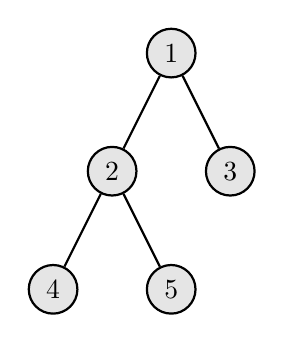
\begin{tikzpicture}
[every node/.style={draw, circle, fill=gray!20!, minimum size=5mm},
thick]
\node{1}
child{node{2} child{node{4}} child{node{5}}}
child{node{3}};
\end{tikzpicture}
\end{figure}
  

\textbf{Output}: \fcj{[[4,5,3],[2],[1]]}
 

\textbf{Explanation}:

Removing the leaves \fcj{[4,5,3]} would result in this tree:

\begin{figure}[H]
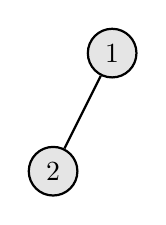
\begin{tikzpicture}
[every node/.style={draw, circle, fill=gray!20!, minimum size=5mm},
thick]
\node{1}
child{node{2}}
child[missing];
\end{tikzpicture}
\end{figure}

Now removing the leaf [2] would result in this tree:

\begin{figure}[H]

\begin{tikzpicture}
[every node/.style={draw, circle, fill=gray!20!, minimum size=5mm},
thick]
\node{1};
\end{tikzpicture}
\end{figure}


Now removing the leaf [1] would result in the empty tree.
\end{flushleft}

\subsection{Find Maximum Height}
We can see the results are sorted by the height of each node, thus we can use the similar recursive approach in finding maximum height

\setcounter{lstlisting}{0}
\begin{lstlisting}[style=customc, caption={DFS}]
vector<vector<int>> findLeaves( TreeNode* root )
{
    vector<vector<int>> ans;
    get_height( root, ans );
    return ans;
}
int get_height( TreeNode* t, vector<vector<int>>& ans )
{
    if( !t )
    {
        return 0;
    }
    //get height of node t
    int h = 1 + ( max )( get_height( t->left, ans ), get_height( t->right, ans ) );
    if( ans.empty() || ( h >= ( int )ans.size() + 1 ) )
    {
        //add another array to hold the values
        ans.emplace_back( vector<int> {} );
    }
    //add t's value to corresponding height
    ans[h - 1].push_back( t->val );
    return h;
}
\end{lstlisting}


% \section{367 --- Valid Perfect Square}
Given a positive integer $ n $, write a function which returns \texttt{true} if $ n $ is a perfect square else \texttt{false}.

\paragraph{Note:} 
\begin{itemize}
\item Do not use any built-in library function such as \texttt{sqrt}.
\end{itemize}

\paragraph{Example 1:}

\begin{flushleft}
\textbf{Input}: 16
\\
\textbf{Output}: \texttt{true}
\end{flushleft}

\paragraph{Example 2:}

\begin{flushleft}
\textbf{Input}: 14
\\
\textbf{Output}: \texttt{false}
\end{flushleft}

\subsection{Newton}
我们需要查找$x^2=n$,即找到函数$f(x)=x^2-n$的root。根据Newton插值法,迭代关系如下
\[
x_{+1} = x_k - \frac{f(x_k)}{f^{'}(x_k)}
\]
将$f(x)$代入上式,可以得到
\begin{align*}
x_{k+1} &= x_k - \frac{x_{k}^2-n}{2x_k}\\
&=\frac{x_k}{2} + \frac{n}{2x_k}
\end{align*}
因此我们从初始值$n$带入上式进行递推测试,直到$x_k^2\leq n$。
\par
另外需要注意的是,由于在计算过程中都是用整数类型,为了避免上述除以2产生误差,因此将除以2放到最后进行,即按照
\[
x_{k+1} = \dfrac{x_k + \dfrac{n}{x_k}}{2}
\]

\setcounter{lstlisting}{0}
\begin{lstlisting}[style=customc, caption={Newton Interpolation}]
bool isPerfectSquare( int num )
{
    //to avoid overflow for int type
    //convert to long long
    auto x = static_cast<long long>( num );
    auto lln = x;

    //newton interpolation
    while( x * x > lln )
    {
        x = ( x + lln / x ) / 2;
    }

    return ( x * x == lln );
}
\end{lstlisting}

\subsection{Binary Search}
这个其实也可以用leftmost binary search来获得。

\begin{lstlisting}[style=customc, caption={Binary Search}]
bool isPerfectSquare( int num )
{
    long long l = 0;
    auto r = static_cast<int>( num );
    auto lln = r;

    //binary search
    while( l < r )
    {
        auto mid = ( l + r ) / 2;

        if( mid * mid < lln )
        {
            l = mid + 1;
        }
        else
        {
            r = mid;
        }
    }

    return l * l == lln;
}
\end{lstlisting}
% \section{368 --- Largest Divisible Subset}
Given a set of distinct positive integers $S$, find the largest subset such that every pair $(S_i, S_j)$ of elements in this subset satisfies: $S_i \bmod S_j = 0$ or $S_j \bmod S_i = 0$.
\par
If there are multiple solutions, return any subset is fine.

\paragraph{Example 1:}

\begin{flushleft}
\textbf{Input}: $ [1,2,3] $
\\
\textbf{Output}: $ [1,2] $ (of course, $ [1,3] $ will also be ok)
\end{flushleft}

\paragraph{Example 2:}

\begin{flushleft}
\textbf{Input}: $ [1,2,4,8] $
\\
\textbf{Output}: $ [1,2,4,8] $
\end{flushleft}

\subsection{Dynamic Programming}
\begin{itemize}
\item 和LIS解法相类似,不过这里返回的不是长度,而是构成最佳结果的elements。
\item 首先需要排序数组,这样只要用后面的数是否能整除前面的数来判断这两个数能不能加入到一个subset中。 
\item 同样用一个array $F$来作为Dynamic Programming的递推数组,其中$F[i]$表示到index $i$所得到的最大的subset的元素个数。和LIS解法一样,对于当前index $i$,都需要从0遍历到$i-1$逐个进行测试
\item 另外用一个array $P$来记录上述过程中以$A[i]$为最后一个元素所能得到的最大subset中上一个$A[i]$能整除的数的index。
\item 用两个变量$\ell$和$t$分别记录当前全局最大的subset的元素个数,以及产生这个最大subset的最大数所在的index。
\item 最后根据数组$P$以及所记录的全局最大subset中的最大数的index,反推出构成全局最大subset的所有elements,加入到输出数组中。
\end{itemize}

\setcounter{algorithm}{0}
\begin{algorithm}[H]
\caption{Dynamic Programming}
\begin{algorithmic}[1]
\Procedure{LargestDivisibleSubset}{$A, L$}
\State $\star$ Sort $A$ by ascending order
\State $\star$ Create an array $F$ with size $L$ and set all elements to $1$ initially
\State $\star$ $F[i]$ is the number elements in the largest subset ending with number $A[i]$. 
\State $\star$ Create an array $P$ with size $L$ and set all element to $+\infty$ initially
\State $\star$ $P[i]$ is the index of last number by which $A[i]$ can be divided in that subset
\State $\ell:=1$ \Comment The number of global largest subset
\State $t:=0$ \Comment The index of largest number in the global largest subset
\For{$i:=1$ to $ L-1 $}
\For{$j:=0$ \textbf{to} $i-1$} \label{368note1}
\If{$ A[i] \bmod A[j] = 0 $}
\If{$F[i] < F[j]+1$} \label{368note2}
\State $F[i]\gets F[j]+1$
\State $P[i]\gets j$
\EndIf  \Comment End If[\ref{368note2}]
\EndIf
\EndFor   \Comment End for loop[\ref{368note1}]
\If{$\ell < F[i]$} \Comment Compare to global value
\State $\ell\gets F[i]$
\State $t\gets i$
\EndIf
\EndFor
\State $\ast$ Get the elements by starting from $t$ and loop through array $P$
\State $s:=\emptyset$ \Comment The result set
\State $\ast$ Add $A[t]$ to $s$
\While{$P[t]\neq +\infty$}
\State $t\gets P[t]$
\State $\ast$ Add $A[t]$ to $s$
\EndWhile
\State \Return $s$
\EndProcedure
\end{algorithmic}
\end{algorithm}

\setcounter{lstlisting}{0}
\begin{lstlisting}[style=customc, caption={Dynamic Programming}]
vector<int> largestDivisibleSubset( vector<int>& nums )
{
    if( nums.empty() )
    {
        return {};
    }

    sort( nums.begin(), nums.end() );

    //the number of elements in the largest subset ending in nums[i]
    vector<int> F( nums.size(), 1 );

    //the index of last number can divide nums[i]
    vector<size_t> pre( nums.size(), nums.size() );

    //global maximum
    int best = 0;
    //nums[best_i] is the largest number in the largest subset
    size_t best_i = 0;

    for( size_t i = 1; i < nums.size(); ++i )
    {
        for( size_t j = 0; j < i; ++j )
        {
            if( ( nums[i] % nums[j] ) == 0 )
            {
                if( F[i] < F[j] + 1 )
                {
                    //found a larger one
                    F[i] = F[j] + 1;
                    //update the index of last number
                    pre[i] = j;
                }
            }
        }

        //compare to global value
        if( F[i] > best )
        {
            best = F[i];
            best_i = i;
        }
    }

    auto x = best_i;

    vector<int> ans;

    //get elements by loop through array pre
    do
    {
        ans.push_back( nums[x] );
        x = pre[x];
    }
    while( x < nums.size() );

    return ans;

}
\end{lstlisting}
% \section{369 --- Plus One Linked List}

\textbf{Medium}

Given a non-negative integer represented as non-empty a singly linked list of digits, plus one to the integer.

You may assume the integer do not contain any leading zero, except the number 0 itself.

The digits are stored such that the most significant digit is at the head of the list.

\paragraph{Example:}

\begin{flushleft}
\textbf{Input}: \fcj{[1,2,3]}

\textbf{Output}: \fcj{[1,2,4]}
\end{flushleft}

\subsection{Find Rightmost Non Nine Node}
We will find the right most non nine node, and change the values of all the nodes after it to zero

\setcounter{lstlisting}{0}
\begin{lstlisting}[style=customc, caption={Sentinel Node}]
ListNode* plusOne( ListNode* head )
{
    auto p = head;
    //find rightmost node which
    //is not 9
    ListNode* non_9 = nullptr;
    while( p )
    {
        if( p->val != 9 )
        {
            non_9 = p;
        }
        p = p->next;
    }
    if( !non_9 )
    {
        //if no such node exists
        //all nodes have value 9
        //thus create a new node before head
        auto new_head = new ListNode( 0 );
        new_head->next = head;
        head = new_head;
        non_9 = head;
    }
    //increments the value of this rightmost
    //non nine node
    non_9->val += 1;
    //change the values of nodes after it
    //to zero
    p = non_9->next;
    while( p )
    {
        p->val = 0;
        p = p->next;
    }
    return head;
}
\end{lstlisting}

\paragraph{Similar Problems}
\begin{itemize}
\item \textbf{66. Plus One}
\end{itemize}


% \section{370 --- Range Addition}

\textbf{Medium}

Assume you have an array of length $n$ initialized with all 0's and are given $k$ update operations.

Each operation is represented as a triplet: \fcj{[startIndex, endIndex, inc]} which increments each element of subarray \fcj{A[startIndex ... endIndex]} (\fcj{startIndex} and \fcj{endIndex} inclusive) with \fcj{inc}.

Return the modified array after all $k$ operations were executed.

\paragraph{Example:}

\begin{flushleft}
\textbf{Input}: \fcj{length = 5}, \fcj{updates = [[1,3,2],[2,4,3],[0,2,-2]]}

\textbf{Output}: \fcj{[-2,0,3,5,3]}

\textbf{Explanation}:

Initial state:

\fcj{[0,0,0,0,0]}

After applying operation \fcj{[1,3,2]}:

\fcj{[0,2,2,2,0]}

After applying operation \fcj{[2,4,3]}:

\fcj{[0,2,5,5,3]}

After applying operation \fcj{[0,2,-2]}:

\fcj{[-2,0,3,5,3]}
\end{flushleft}

\subsection{Prefix Sum}
Apply update \fcj{[start, end]} with value $n$, we can update \fcj{[start, length-1]} with value $n$ and then update \fcj{[end+1, length-1]} with value $-n$.

There is only one read query on the entire range, and it occurs at the end of all update queries. Additionally, the order of processing update queries is irrelevant.

Cumulative sums operations apply the effects of past elements to the future elements in the sequence.

\setcounter{lstlisting}{0}
\begin{lstlisting}[style=customc, caption={Prefix Sum}]
vector<int> getModifiedArray( int length, vector<vector<int>>& updates )
{
    vector<int> ans( length, 0 );
    for( const auto& update : updates )
    {
        //set arr[start] = arr[start] + n
        ans[update[0]] += update[2];
        //set arr[end+1] = arr[end+1]-n
        if( update[1] < length - 1 )
        {
            ans[update[1] + 1] -= update[2];
        }
    }
    //apply cumulative sum
    // partial_sum applies the following operation (by default) for the parameters {x[0], x[n], y[0]}:
    // y[0] = x[0]
    // y[1] = y[0] + x[1]
    // y[2] = y[1] + x[2]
    // ...  ...  ...
    // y[n] = y[n-1] + x[n]
    partial_sum( begin( ans ), end( ans ), begin( ans ) );
    return ans;
}
\end{lstlisting}

\paragraph{Similar Problems}
\begin{itemize}
\item \textbf{598. Range Addition II}
\end{itemize}
% \section{371 --- Sum of Two Integers}
Calculate the sum of two integers $ a $ and $ b $, but you are not allowed to use the operator $ + $ and $ - $.

\paragraph{Example 1:}

\begin{flushleft}
\textbf{Input}: $ a = 1 $, $ b = 2 $
\\
\textbf{Output}: 3
\end{flushleft}

\paragraph{Example 2:}

\begin{flushleft}
\textbf{Input}: $ a = -2 $, $ b = 3 $
\\
\textbf{Output}: 1
\end{flushleft}


% \section{372 --- Super Pow}
Your task is to calculate $ a^b \bmod 1337$ where $ a $ is a positive integer and $ b $ is an extremely large positive integer given in the form of an array.

\paragraph{Example 1:}

\begin{flushleft}
\textbf{Input}:$  a = 2 $, $ b = [3] $
\\
\textbf{Output}: 8
\end{flushleft}

\paragraph{Example 2:}

\begin{flushleft}
\textbf{Input}:$  a = 2 $, $ b = [1,0] $
\\
\textbf{Output}: 1024
\end{flushleft}

\subsection{Digital Logarithmic}
\begin{enumerate}
\item 首先注意到$(x\times y)\bmod k = (x\bmod k)\times (y\mod k)$ \item 根据1, 还可以得到$(a^b)\bmod k = (a^{b-c}\bmod k)\times (a^c\bmod k)$。例如$(a^{12345}\bmod k) = (a^{12340}\bmod k)\times (a^5\bmod k)$。
\item 而$a^{12340}\bmod k = (a^{1234}\bmod k)^{10}$。
\item 依据上述分析,假设$f(a, b) = (a^b)\bmod k$,那么$f(a,b) = f(f(a, b/10), 10)\times f(a, b\bmod 10)$。而由于$b$在题目中是以数组的形式给出,因此只要从数组最后面的数字往前面递推即可。
\end{enumerate}

\setcounter{algorithm}{0}
\begin{algorithm}[H]
\caption{Digital Logarithmic}
\begin{algorithmic}[1]
\Procedure{SuperPow}{$a, b, L$}
\If{$b$ is empty}
\State \Return 1
\EndIf
\State $t:=b[L-1]$
\State $\star$ Remove the last number from $b$, so $b$'s length decrease to $L-1$
\State $u:$=\Call{SuperPow}{$a, b, L-1$} \Comment $(a^{b/10}\bmod 1337)$
\State $x:=$\Call{GetMod}{$ u , 10$} \Comment $ (a^{b/10}\bmod 1337) ^ {10}\bmod 1337 $
\State $y:=$\Call{GetMod}{$ a, t $} \Comment $a^{(b\bmod 10)}\bmod 1337$
\State \Return $(x\times y)\bmod 1337$ \Comment Need to modular 1337 again to ensure the result is less than 1337
\algstore{372algo}
\end{algorithmic}
\end{algorithm}
\begin{algorithm}[H]
\begin{algorithmic}[1]
\algrestore{372algo}
\EndProcedure
\end{algorithmic}
\end{algorithm}

Function \texttt{GetMod}则计算$(a^e)\bmod 1337$,其中$e$是个位数。

\begin{algorithm}[H]
\caption{Get $a^e$ modular}
\begin{algorithmic}[1]
\Function{GetMod}{$a, e$}
\State $c:=1$
\For{$w:=1$ \textbf{to} $e$}
\State $c\gets (c\times a)\bmod 1337$
\EndFor
\State \Return $c$
\EndFunction
\end{algorithmic}
\end{algorithm}

\setcounter{lstlisting}{0}
\begin{lstlisting}[style=customc, caption={Digital Modular}]
int superPow( int a, vector<int>& b )
{
    if( b.empty() )
    {
        return 1;
    }

    int t = b.back();
    b.pop_back();

    int u = superPow( a, b ); //a^(b/10) % 1337

    return ( get_mod( u, 10 ) * get_mod( a, t ) ) % 1337;

}

int get_mod( int a, int b )
{
    //get (a^b)%k

    long long c = 1;

    for( int e = 0; e < b; ++e )
    {
        c = ( ( c * a ) % 1337 );

    }

    return c;
}
\end{lstlisting}
% \section{373 --- Find K Pairs with Smallest Sums}
You are given two integer arrays $ A $ and $ B $ sorted in ascending order and an integer $ k $.
\par
Define a pair $ (u,v) $ which consists of one element from the first array and one element from the second array.
\par
Find the $ k $ pairs $ (u_1,v_1),\; (u_2,v_2), \; \ldots,\;  (u_k,v_k) $ with the smallest sums.

\paragraph{Example 1:}

\begin{flushleft}
\textbf{Input}: $ A = [1,7,11] $, $ B = [2,4,6] $, $ k = 3 $
\\
\textbf{Output}: $[\;[1,2],[1,4],[1,6]\;]$ 
\\
\textbf{Explanation}: The first 3 pairs are returned from the sequence: 
            $  [1,2],\;[1,4],\;[1,6],\;[7,2],\;[7,4],\;[11,2],\;[7,6],\;[11,4],\;[11,6] $
\end{flushleft}

\paragraph{Example 2:}

\begin{flushleft}
\textbf{Input}:$  A = [1,1,2] $, $ B = [1,2,3] $, $ k = 2 $
\\
\textbf{Output}: $ [1,1] $, $ [1,1] $
\\
\textbf{Explanation}: The first 2 pairs are returned from the sequence: 
             $ [1,1],\;[1,1],\;[1,2],\;[2,1],\;[1,2],\;[2,2],\;[1,3],\;[1,3],\;[2,3] $
\end{flushleft}
             
             
\paragraph{Example 3:}

\begin{flushleft}
\textbf{Input}: $A = [1,2]$, $B = [3]$, $ k = 3 $
\\
\textbf{Output}: $ [1,3],\;[2,3] $
\\

\textbf{Explanation}: All possible pairs are returned from the sequence: $ [1,3],\;[2,3] $
\end{flushleft}

\subsection{Priority Queue}
\begin{enumerate}
\item 创建一个minimum priority queue $ Q $,其元素为$A$和$B$中的index pair $ (i,j) $,然后能产生最小的$A[i]+B[j]$的index pair在栈顶。
\item 接着向$Q$中加入$(0,0)$,$ (1,0) $,$\ldots$直到$(\min(k, L_A),0)$。相当于把$A$中前$\min(k, L_A)$个数与$B[0]$加入到了$Q$中,由于$B[0]$是$B$中最小的,因此这样就把$B$中元素与$A$中元素之和的$\min(k, L_A)$个最小的放入$ Q $中。
\item 然后开始逐步将$Q$中的元素弹出,加入到输出结果数组中,在弹出的元素中,将对应$B$的index increment,然后重新加入$Q$中排序,重复这个过程直到$k$为零或者$Q$为empty。
\end{enumerate}

\setcounter{lstlisting}{0}
\begin{lstlisting}[style=customc, caption={Priority Queue}]
vector<vector<int>> kSmallestPairs( vector<int>& nums1, vector<int>& nums2, int k )
{
    if( nums1.empty() || nums2.empty() || ( k == 0 ) )
    {
        return {};
    }
    //define comparison functino to sort when push into queue
    auto cmp = [&nums1, &nums2]( const pair<int, int>& p1, const pair<int, int>& p2 )
    {
        return nums1[p1.first] + nums2[p1.second] >
               nums1[p2.first] + nums2[p2.second];
    };
    priority_queue<pair<int, int>, vector<pair<int, int>>, decltype( cmp )> pq( cmp );
    vector<vector<int>> ans( k, vector<int>( 2 ) );
    int l1 = (int)nums1.size();
    int l2 = (int)nums2.size();
    int max_i = ( min )( l1, k );
    //add max_i index in A and 0 index in B to the queue
    for( int i = 0; i < max_i; ++i )
    {
        pq.emplace( i, 0 );
    }
    int ki = 0;
    while( ( ki < k ) && !pq.empty() )
    {
        auto i1 = pq.top().first;
        auto i2 = pq.top().second;
        pq.pop();
        ans[ki][0] = nums1[i1];
        ans[ki][1] = nums2[i2];
        ++ki;
        //increment index in B
        //so that we can get possible smaller sum from
        //other elements in B
        if( i2 + 1 < l2 )
        {
            pq.emplace( i1, i2 + 1 );
        }
    }
    if( ki < k )
    {
        ans.resize( ki );
    }
    return ans;
}
\end{lstlisting}

\paragraph{Similar Problems}
\begin{itemize}
\item \textbf{378. Kth Smallest Element in a Sorted Matrix}
\item \textbf{719. Find K-th Smallest Pair Distance}
\end{itemize}
% \section{374 --- Guess Number Higher or Lower}
We are playing the Guess Game. The game is as follows:
\par
I pick a number from 1 to $ n $. You have to guess which number I picked.
\par
Every time you guess wrong, I'll tell you whether the number is higher or lower.
You call a pre-defined API \texttt{guess} which returns 3 possible results ($ -1 $, 1, or 0):
\begin{itemize}
\item $ -1 $ : My number is lower
\item  1 : My number is higher
\item  0 : Congrats! You got it!
\end{itemize}

\paragraph{Example:}

\begin{flushleft}
\textbf{Input}: $  n = 10 $, pick $ = 6 $
\\
\textbf{Output}: 6
\end{flushleft}

\subsection{Binary Search}
典型的binary search。

\setcounter{lstlisting}{0}
\begin{lstlisting}[style=customc, caption={Binary Search}]
int guessNumber( int n )
{
    int l = 1;
    int r = n;

    while( l <= r )
    {
        //not use (l+r)/2 to avoid
        //type overflow for (l+r)
        int mid = l + ( r - l ) / 2;
        int x = guess( mid );

        if( x < 0 )
        {
            r = mid - 1;
        }
        else if( x > 0 )
        {
            l = mid + 1;
        }
        else
        {
            return mid;
        }

    }

    return -1;

}
\end{lstlisting}
\section{375 --- Guess Number Higher or Lower II}
We are playing the Guess Game. The game is as follows:

\begin{itemize}
\item I pick a number from 1 to $ n $. You have to guess which number I picked.

\item Every time you guess wrong, I'll tell you whether the number I picked is higher or lower.

\item However, when you guess a particular number $ x $, and you guess wrong, you pay \$$x$. You win the game when you guess the number I picked.
\end{itemize}

\paragraph{Example:}

\begin{flushleft}
$ n = 10 $, I pick 8.
\\
First round:  You guess 5, I tell you that it's higher. You pay \$5.
\\
Second round: You guess 7, I tell you that it's higher. You pay \$7.
\\
Third round:  You guess 9, I tell you that it's lower. You pay \$9.
\\
Game over. 8 is the number I picked.
\\
You end up paying $\$5 + \$7 + \$9 = \$21$
\end{flushleft}

Given a particular $n \geq 1$, find out how much money you need to have to guarantee a win.

\subsection{MinMax Algorithm}
\begin{itemize}
\item 建立一个二维的数组$F$用于Dynamic Programming,其中$F[i][j]$表示从数字$i$到$j$之间猜中任意一个数字最少需要花费的钱数。
\item 需要遍历每一段可能的区间$[x, y]$,用$t$表示全局最小值,然后遍历$ [x,y] $的中每一个数字$k$,猜中$k$所需要花费的money $u_k = k + \max(F[x][k - 1], F[k + 1][i])$,也就是是将区间$ [x,y] $在每一个位置$k$都分为两段,然后取当前位置的花费加上左右两段中较大的花费之和。
\item 取两者之间的较大值的原因是在MinMax中,需要从最坏的情况下获得最佳值。
\item 最后取$\underbrace{\min}_{x< k < y}u_k$作为$F[x][y]$。
\item 如果$y=x+1$,很显然$F[x][y]=x$。
\end{itemize}

\setcounter{algorithm}{0}
\begin{algorithm}[H]
\caption{Dynamic Programming}
\begin{algorithmic}[1]
\Procedure{GetMoneyAmount}{$n$}
\State $\star$ 创建二维数组$F$作为递推数组,大小为$n\times n$
\State $ \star $We use $[0,n-1]$ to represent integers in $[1,n]$
\For{$i:=0$ \textbf{to} $n-1$}
\State $F[i][i]=0$ \Comment Since $i$ is the guess number, so no money is needed
\EndFor
\For{$i:=0$ \textbf{to} $n-2$}
\State $F[i][i+1]=i+1$ \Comment We try to guess the smaller number $i+1$ to put less money $i+1$
\EndFor
\For{$\ell:=3$ \textbf{to} $n$}  \label{375note1}
\For{$x:=0$ \textbf{to} $n-\ell$} \label{375note2}
\State $y:=x+\ell-1$ \Comment range $[x,y]$
\State $F[x][y] \gets +\infty$
\For{$k:=x+1$ \textbf{to} $y-1$} \label{375note3}
\State $u := k+1+\max(F[x][k-1], F[k+1][y])$ \Comment The money needed to guess number $k+1$
\State $F[x][y]\gets \min(F[x][y], u)$ \Comment Update the money to guess number in range $[x,y]$
\EndFor \Comment End loop[\ref{375note3}]
\EndFor \Comment End loop[\ref{375note2}]
\EndFor \Comment End loop[\ref{375note1}]
\State \Return $F[0][n-1]$
\EndProcedure
\end{algorithmic}
\end{algorithm}

\setcounter{lstlisting}{0}
\begin{lstlisting}[style=customc, caption={Dynamic Programming}]
int getMoneyAmount( int n )
{
    //we use [0,n-1] to represent range [1,n]
    vector<vector<int>> F( n, vector<int>( n, INT_MAX ) );

    for( int i = 0; i < n; ++i )
    {
        //i is the correct guessed number
        //no money is needed
        F[i][i] = 0;
    }

    for( int i = 0; i < n - 1; ++i )
    {
        //we want to guess smaller number i+1
        //to put less money i+1
        //notice we use [0,n-1] to represent range [1,n]
        F[i][i + 1] = i + 1;
    }

    for( int l = 3; l <= n; ++l )
    {
        for( int x = 0; x + l - 1 < n; ++x )
        {
            int y = x + l - 1;

            //find minimum money for guessing number in range
            //[x+1][y+1]
            for( int k = x + 1; k < y; ++k )
            {
                //for each number k+1
                //the cost to guess this number
                int u = k + 1 + ( max )( F[x][k - 1], F[k + 1][y] );
                F[x][y] = ( min )( F[x][y], u );
            }
        }
    }

    return F[0][n - 1];
}
\end{lstlisting}
% \section{376 --- Wiggle Subsequence}
A sequence of numbers is called a \textbf{wiggle sequence} if the differences between successive numbers strictly alternate between positive and negative. The first difference (if one exists) may be either positive or negative. A sequence with fewer than two elements is trivially a wiggle sequence.

For example, \fcj{[1,7,4,9,2,5]}  is a wiggle sequence because the differences  \fcj{(6,-3,5,-7,3)}  are alternately positive and negative. In contrast, \fcj{[1,4,7,2,5]} and \fcj{[1,7,4,5,5]} are not wiggle sequences, the first because its first two differences are positive and the second because its last difference is zero.

Given a sequence of integers $A$, return the length of the longest subsequence that is a wiggle sequence. A subsequence is obtained by deleting some number of elements (eventually, also zero) from the original sequence, leaving the remaining elements in their original order.

\paragraph{Example 1:}

\begin{flushleft}
\textbf{Input}: \fcj{[1,7,4,9,2,5]}

\textbf{Output}: 6

\textbf{Explanation}: The entire sequence is a wiggle sequence.
\end{flushleft}

\paragraph{Example 2:}

\begin{flushleft}
\textbf{Input}: \fcj{[1,17,5,10,13,15,10,5,16,8]}

\textbf{Output}: 7

\textbf{Explanation}: There are several subsequences that achieve this length. One is \fcj{[1,17,10,13,10,16,8]}.
\end{flushleft}

\paragraph{Example 3:}

\begin{flushleft}
\textbf{Input}: \fcj{[1,2,3,4,5,6,7,8,9]}
\\
\textbf{Output}: 2
\end{flushleft}

\paragraph{Follow up:}
\begin{itemize}
\item Can you do it in $ O(n) $ time?
\end{itemize}

\subsection{Linear Dynamic Programming}
采用Dynamic Programming,利用两个递推数组$U$ and $D$。
\begin{enumerate}
\item $U[i]$ is the length of a longest wiggle subsequence of $A[0],\ldots,A[i]$, with a \textbf{positive} difference between its last two numbers. This subsequence may or may not include $A[i]$ and there may be several such subsequences (of the same length). 称这种类型的subsequence为$U$.
\item $D[i]$ is the length of a longest wiggle subsequence of $A[0],\ldots,A[i]$, with a \textbf{negative} difference between its last two numbers. This subsequence may or may not include $A[i]$ and there may be several such subsequences (of the same length). 称这种类型的subsequence为$D$.
\end{enumerate}
然后可以得到如下的递推关系式
\begin{enumerate}
%那么可以用$A[i]$构成一个更长的subsequence $U$
\item 如果$A[i]>A[i-1]$,假设有一个类型为$D$的subsequence $S_d$ from $A[0],\ldots,A[i-1]$,其length为$D[i-1]$,而$A[x]$ is the last element of $S_d$。那么有两种情况
\begin{enumerate}
\item If $A[i] > A[x]$,显然可以把$A[i]$加入$S_d$从而构成一个类型为$U$的subsequence。
\item Otherwise, since $A[x]$ cannot be $A[i-1]$ (because $A[i-1] < A[i]\leq A[x]$), replace $A[x]$ by $A[i-1]$ gives another type $D$ subsequence $\hat{S}_d$ with same length. And then we can also add $A[i]$ to $\hat{S}_d$ to get a subsequence of type $U$.
\end{enumerate}
Both cases give $U[i]=D[i-1]+1$,而$D[i]$显然是不变的,所以$D[i] = D[i-1]$
\item 类似的,如果$A[i] < A[i-1]$,可以得到$D[i] = U[i-1]+1$,$U[i]=U[i-1]$。
\item 如果$A[i]=A[i-1]$,显然不会改变已有的type $U$和$D$ subsequences,因此$U[i]=U[i-1]$, $D[i]=D[i-1]$
\end{enumerate}

\setcounter{lstlisting}{0}
\begin{lstlisting}[style=customc, caption={Dynamic Programming}]
int wiggleMaxLength( vector<int>& nums )
{
    if( nums.empty() )
    {
        return 0;
    }

    vector<int> U( nums.size(), 1 );
    vector<int> D( nums.size(), 1 );

    for( size_t i = 1; i < nums.size(); ++i )
    {
        if( nums[i] > nums[i - 1] )
        {
            U[i] = D[i - 1] + 1;
            D[i] = D[i - 1];
        }
        else if( nums[i] < nums[i - 1] )
        {
            //D can be longer by adding nums[i]
            //to subsquence U
            D[i] = U[i - 1] + 1;
            U[i] = U[i - 1];
        }
        else
        {
            //no changes to the lengths of U and D
            U[i] = U[i - 1];
            D[i] = D[i - 1];
        }
    }

    return ( max )( U.back(), D.back() );
}
\end{lstlisting}

\subsection{O(1) Memory Dynamic Programming}
从上面的递推式可以看到,$U[i]$和$D[i]$仅仅取决于$U[i-1]$和$D[i-1]$,因此可以把数组替换为两个变量$U$和$D$。
\begin{lstlisting}[style=customc, caption={$O(1)$ Memory Dynamic Programming}]
int wiggleMaxLength( vector<int>& nums )
{
    if( nums.empty() )
    {
        return 0;
    }
    //the maximum length of type U subsequence so far
    int U = 1;
    //the maximum length of type D subsequence so far
    int D = 1;
    for( size_t i = 1; i < nums.size(); ++i )
    {
        if( nums[i] > nums[i - 1] )
        {
            //nums[i] can make a longer U subsequence
            U = D + 1;
        }
        else if( nums[i] < nums[i - 1] )
        {
            //nums[i] can make a longer D subsequence
            D = U + 1;
        }
    }
    return ( max )( U, D );
}
\end{lstlisting}
% \section{377 --- Combination Sum IV}
Given an integer array $A$ with all positive numbers and no duplicates, find the number of possible combinations that add up to a positive integer target $T$.

\paragraph{Example:}

\begin{flushleft}
\textbf{Input}: $A = [1, 2, 3]$, $T = 4$
\\
\textbf{Output}: 7
\\
\textbf{Explanation}: The possible combination ways are:
\begin{table}[H]
\begin{tabular}{llll}
1 & 1 & 1 & 1\\
1 & 1 & 2 & \\
1 & 2 & 1  & \\
1 & 3  &  & \\
2 & 1 & 1 & \\
2 & 2 &  & \\
3 & 1 &  & 
\end{tabular}
\end{table}
Note that different sequences are counted as \textbf{different} combinations.
\end{flushleft}

\paragraph{Follow up:}
\begin{itemize}
\item What if negative numbers are allowed in the given array?
\item How does it change the problem?
\item What limitation we need to add to the question to allow negative numbers?
\end{itemize}

\subsection{Dynamic Programming}
We need a DP array $F$, where $F[i]$ means the count of possible combinations add up to $i$.

\setcounter{lstlisting}{0}
\begin{lstlisting}[style=customc, caption={DP}]
int combinationSum4( vector<int>& nums, int target )
{
    //we need a slove space of [0, target];
    vector<int> F( target + 1, 0 );
    //Base case: we have only one way to achieve target zero
    //i.e. select nothing from nums
    F[0] = 1;
    //for each element in the solve space
    //try possible number from input array
    for( int i = 1; i <= target; ++i )
    {
        for( int n : nums )
        {
            if( i >= n )
            {
                F[i] += F[i - n];
            }
        }
    }
    return F.back();
}
\end{lstlisting}

However, in some cases, if we use \fcc{int} type, the result will be datatype overflow. We need to skip impossible target with recursion and memorization

\begin{lstlisting}[style=customc, caption={DP With Memo}]
int combinationSum4( vector<int>& nums, int target )
{
    unordered_map<int, int> m;
    return dfs( target, nums, m );
}
//recursion helper function
int dfs( int t, vector<int>& nums, unordered_map<int, int>& m )
{
    if( t < 0 )
    {
        return 0;
    }
    if( t == 0 )
    {
        return 1;
    }
    auto it = m.find( t );
    if( it != m.end() )
    {
        return it->second;
    }
    int count = 0;
    //test each number of input array
    for( int n :  nums )
    {
        //accumulate the result for each target (t-n)
        count += dfs( t - n, nums, m );
    }
    m.emplace( t, count );
    return count;
}
\end{lstlisting}
 
\subsection{Follow Up}
If negative numbers exist in input array, then the combinations could be infinite length. If we limit the length of the combination sequence, the problem will have a finite solution.

% \section{378 --- Kth Smallest Element in a Sorted Matrix}
Given a $ n \times n $ matrix $M$ where each of the rows and columns are sorted in ascending order, find the $k$th smallest element in the matrix.
\par
Note that it is the $k$th smallest element in the sorted order, not the $k$th distinct element.

\paragraph{Example:}
\begin{flushleft}
\textbf{Input}: $k=8$ and $M$ is 
\begin{table}[H]
\begin{tabular}{ccc}
1 & 5 & 9\\
10 & 11 & 13\\
12 & 13 & 15
\end{tabular}
\end{table}
\textbf{Output}: 13
\end{flushleft}

\paragraph{Note: }
\begin{itemize}
\item You may assume $ k $ is always valid, $ 1 \leq k \leq n^2 $.
\end{itemize}

\subsection{Binary Search}
在binary search中,首先需要定义Search Space。对于数组搜索来说,有两种类型的Search Space: index和range。大部分情况下,当数组是在一个方向上是sorted,就用index作为Search Space。而当数组没有排序,而需要寻找某个特定数时,需要用range作为Search Space。这里的range指的是数组中最小和最大数之间的range。
\par
这道题的Search Space只能是用range,这是因为整个matrxi实际上是在row和column两个方向上是sorted,但row与column之间并不是,所以也就找不到一个线性的方式来建立某个数和其index的映射。
\par
采用range作为search space,
\begin{enumerate}
\item 首先以当前range的中间数作为target,在matrix中寻找不大于这个target的元素的个数$\delta$,如果$\delta$小于$k$,说明target小了,将range的左边界更新为这个中间数加1。
\item 而如果$\delta$大于或者等于$k$,说明目标数大了,将range的右边界更新为中间数。
\item 而在matrix中计算$\delta$时,最佳的方法是从$M[C-1][0]$开始,逐行逐列的搜索。假设当前搜索到了位置$(r,c)$,
\begin{itemize}
\item 如果$M[r][c]$比目标值小,。由于column $c$中,小于$r$的所有元素都比$M[r][c]$小,因此$\delta$增加$r+1$(因为$r$是从0开始的),另外,increment column $c$,即$c\gets c+1$,即向右移动。
\item 反之,则decrement $r$,即向上移动。
\end{itemize}
\end{enumerate}
可以看到上面的过程其实就是leftmost binary search,只不过Search Space是range,不是index。需要在range中找到第一个数,使得range中小于等于这个数的count为$k$。


\setcounter{lstlisting}{0}
\begin{lstlisting}[style=customc, caption={Binary Search}]
int kthSmallest( vector<vector<int>>& matrix, int k )
{
    int l = matrix[0][0];
    int r = matrix.back().back();

    //leftmost binary search
    //search space is range
    while( l < r )
    {
        int mid = l + ( r - l ) / 2;
        int count = get_numbers( matrix, mid );

        if( count < k )
        {
            l = mid + 1;
        }
        else
        {
            r = mid;
        }
    }

    return l;

}
//Helper function
//get count of numbers that are no larger than target in matrix
int get_numbers( vector<vector<int>>& matrix, int target )
{
    //matrix size is n x n
    int n = static_cast<int>( matrix[0].size() );

    int c = 0;
    int r = n - 1;
    int count = 0;

    while( ( r >= 0 ) && ( c < n ) )
    {
        if( matrix[r][c] <= target )
        {
            count += ( r + 1 );
            ++c;
        }
        else
        {
            --r;
        }
    }

    return count;
}
\end{lstlisting}

We can use iterator to simplify some code

\begin{lstlisting}[style=customc, caption={STL Iterator}]
int kthSmallest( vector<vector<int>>& matrix, int k )
{
    //the search space is [lo, hi]
    int lo = matrix[0][0];
    int hi = matrix.back().back();
    //get count of elements inside matrix
    //which is less than x
    auto less_count = [ &matrix ]( int x )
    {
        int count = 0;
        auto rp = rbegin( matrix );
        size_t col{};
        while( ( rp != matrix.rend() ) && ( col < matrix[0].size() ) )
        {
            if( ( *rp )[col] <= x )
            {
                //from first row to current row
                //the element at this column
                //are all no larger than x
                //notice, we want to get count of rows from 0 to current row
                //matrix.rend() is the row before 0, and rp is current row
                //so distance( rp, matrix.rend() ) give the number of rows
                count += ( int ) distance( rp, matrix.rend() );
                ++col;
            }
            else
            {
                ++rp;
            }
        }
        return count;
    };
    //leftmost binary search
    while( lo < hi )
    {
        auto mid = lo + ( hi - lo ) / 2;
        auto count = less_count( mid );
        if( count < k )
        {
            lo = mid + 1;
        }
        else
        {
            hi = mid;
        }
    }
    return lo;
}
\end{lstlisting}

\paragraph{Similar Problems}
\begin{itemize}
\item \textbf{373. Find K Pairs with Smallest Sums}
\item \textbf{668. Kth Smallest Number in Multiplication Table}
\item \textbf{719. Find K-th Smallest Pair Distance}
\item \textbf{786. K-th Smallest Prime Fraction}
\end{itemize}
% \section{379 --- Design Phone Directory}

\textbf{Medium}

Design a Phone Directory which supports the following operations:

\begin{itemize}
\item \fcc{get}: Provide a number which is not assigned to anyone.

\item \fcc{check}: Check if a number is available or not.

\item \fcc{release}: Recycle or release a number.
\end{itemize}

\paragraph{Example:}

\begin{flushleft}
\fcc{// Init a phone directory containing a total of 3 numbers: 0, 1, and 2.}

\fcc{PhoneDirectory directory = new PhoneDirectory(3);}

\fcc{// It can return any available phone number. Here we assume it returns 0.}

\fcc{directory.get();}

\fcc{// Assume it returns 1.}

\fcc{directory.get();}

\fcc{// The number 2 is available, so return true.}

\fcc{directory.check(2);}

\fcc{// It returns 2, the only number that is left.}

\fcc{directory.get();}

\fcc{// The number 2 is no longer available, so return false.}

\fcc{directory.check(2);}

\fcc{// Release number 2 back to the pool.}

\fcc{directory.release(2);}

\fcc{// Number 2 is available again, return true.}

\fcc{directory.check(2);}
\end{flushleft}

\subsection{Queue With Hash Set}
In order to achieve average $O(1)$ time complexity for each operation, we have to push each number into the queue.

\setcounter{lstlisting}{0}
\begin{lstlisting}[style=customc, caption={Queue}]
class PhoneDirectory
{
public:
    /** Initialize your data structure here
        @param maxNumbers - The maximum numbers that can be stored in the phone directory. */
    PhoneDirectory( int maxNumbers )
    {
        //add all numbers into the queue
        for( int i = 0; i < maxNumbers; ++i )
        {
            q.push( i );
        }
    }
    /** Provide a number which is not assigned to anyone.
        @return - Return an available number. Return -1 if none is available. */
    int get()
    {
        if( q.empty() )
        {
            //we have used all numbers
            return -1;
        }
        int num = q.front();
        q.pop();
        used.insert( num );
        return num;
    }
    /** Check if a number is available or not. */
    bool check( int number )
    {
        return used.find( number ) == used.end();
    }
    /** Recycle or release a number. */
    void release( int number )
    {
        if( used.find( number ) == used.end() )
        {
            //this number is not used
            //no need to recycle
            return;
        }
        q.push( number );
        used.erase( number );
    }
    queue<int> q;
    unordered_set<int> used;
};
\end{lstlisting} 
% \section{380 --- Insert Delete GetRandom O(1)}
Design a data structure that supports all following operations in average O(1) time.

\begin{lstlisting}[style=customc]
insert(val) //Inserts an item val to the set if not already present.
remove(val) //Removes an item val from the set if present.
getRandom // Returns a random element from current set of elements. Each element must have the same probability of being returned.
\end{lstlisting}

\paragraph{Example:}

\begin{lstlisting}[style=customc]
// Init an empty set.
RandomizedSet randomSet = new RandomizedSet();

// Inserts 1 to the set. Returns true as 1 was inserted successfully.
randomSet.insert(1);

// Returns false as 2 does not exist in the set.
randomSet.remove(2);

// Inserts 2 to the set, returns true. Set now contains [1,2].
randomSet.insert(2);

// getRandom should return either 1 or 2 randomly.
randomSet.getRandom();

// Removes 1 from the set, returns true. Set now contains [2].
randomSet.remove(1);

// 2 was already in the set, so return false.
randomSet.insert(2);

// Since 2 is the only number in the set, getRandom always return 2.
randomSet.getRandom();
\end{lstlisting}

\subsection{Hash Map}
\begin{itemize}
\item Maintain one array $X$ and one hash map $M$.
\item Use $X$ to store numbers and $M$ to map the number and its index in $X$
\item \texttt{Insert} operation: 
\begin{enumerate}
\item Check if the number exists in $M$. If Yes, then return \texttt{false}。Otherwise, we insert the number into the end of $X$, and insert to $M$ with its index in $X$.
\end{enumerate}
\item \texttt{Delete} operation:
\begin{enumerate}
\item To delete the number from the array $X$ in $O(1)$ time, swap the number with the last number. 
\item Since the number's index is changed, we also need to modify its mapping in $M$.
\item Then, we just only delete the last number in $X$.
\end{enumerate}
\item \texttt{getRandom} operation: Generate a random integer $i$ between $[0, \lvert X\rvert-1]$, and returns the number at index $i$.
\end{itemize}

\setcounter{lstlisting}{0}
\begin{lstlisting}[style=customc, caption={Hash Map}]
class RandomizedSet
{
public:
    /** Initialize your data structure here. */
    RandomizedSet()
    {
    }

    /** Inserts a value to the set. Returns true if the set did not already contain the specified element. */
    bool insert( int val )
    {
        auto it = M.find( val );
        if( it != M.end() )
        {
            return false;
        }

        X.push_back( val );
        M.emplace( val, X.size() - 1 );

        return true;
    }

    /** Removes a value from the set. Returns true if the set contained the specified element. */
    bool remove( int val )
    {
        auto it = M.find( val );
        if( it == M.end() )
        {
            return false;
        }

        auto pos = it->second;
        if( pos != X.size() - 1 )
        {
            //Copy the last element
            //to the position of val
            X[pos] = X.back();
            auto it_back = M.find( X.back() );
            it_back->second = pos;
        }

        //remove the last element
        X.pop_back();
        M.erase( it );

        return true;
    }

    /** Get a random element from the set. */
    int getRandom()
    {
        return X[rand() % X.size()];
    }

    vector<int> X;
    unordered_map<int, size_t> M;
};
\end{lstlisting}
% \section{381 --- Insert Delete GetRandom O(1) - Duplicates allowed}
Design a data structure that supports all following operations in average $ O(1) $ time.

\paragraph{Note:} 
\begin{itemize}
\item Duplicate elements are allowed.
\end{itemize}


\begin{lstlisting}[style=customc]
insert(val): //Inserts an item val to the collection.
remove(val): //Removes an item val from the collection if present.
getRandom: //Returns a random element from current collection of elements. The probability of each element being returned is linearly related to the number of same value the collection contains.
\end{lstlisting}

\paragraph{Example:}

\begin{lstlisting}[style=customc]
// Init an empty collection.
RandomizedCollection collection = new RandomizedCollection();

// Inserts 1 to the collection. Returns true as the collection did not contain 1.
collection.insert( 1 );

// Inserts another 1 to the collection. Returns false as the collection contained 1. Collection now contains [1,1].
collection.insert( 1 );

// Inserts 2 to the collection, returns true. Collection now contains [1,1,2].
collection.insert( 2 );

// getRandom should return 1 with the probability 2/3, and returns 2 with the probability 1/3.
collection.getRandom();

// Removes 1 from the collection, returns true. Collection now contains [1,2].
collection.remove( 1 );

// getRandom should return 1 and 2 both equally likely.
collection.getRandom();
\end{lstlisting}

\subsection{Hash Map}
\begin{itemize}
\item Similar to problem 380. To deal with duplicate, we change the value type of hash map to hash set.
\item When remove a value $v$
\begin{enumerate}
\item Find if one of $v$ is at the end of the array $X$. If it is, remove the end index from $v$'s positions.
\item Otherwise, put the last element of $X$ into a position of $v$. We choose the first element in $v$'s hash set as this position, and then remove the end index for last element's positions after inserting the new position.
\end{enumerate}
\end{itemize}

\setcounter{lstlisting}{0}
\begin{lstlisting}[style=customc, caption={Similar to 380}]
class RandomizedCollection
{
public:
    /** Initialize your data structure here. */
    RandomizedCollection()
    {
    }

    /** Inserts a value to the collection. Returns true if the collection did not already contain the specified element. */
    bool insert( int val )
    {
        X.push_back( val );

        auto it = M.find( val );

        if( it == M.end() )
        {
            //insert new val
            M.emplace( val, initializer_list<size_t> {X.size() - 1} );
            return true;
        }

        //val exists, just insert to its positions
        it->second.insert( X.size() - 1 );

        return false;
    }

    /** Removes a value from the collection. Returns true if the collection contained the specified element. */
    bool remove( int val )
    {
        auto it_val = M.find( val );
        if( it_val == M.end() )
        {
            return false;
        }

        //find if val has position equal to last index of X
        auto it_val_idx = it_val->second.find( X.size() - 1 );
        if( it_val_idx == it_val->second.end() )
        {
            //find the last element of X in M
            int last = X.back();
            auto it_last = M.find( last );
            size_t i_val = *( it_val->second.begin() );

            //put last at index i_val
            X[i_val] = last;
            //add the new position into the positions
            it_last->second.insert( i_val );

            //remove the end index from last's positions
            it_last->second.erase( X.size() - 1 );

            //remove begin element from val's positions
            it_val->second.erase( it_val->second.begin() );
        }
        else
        {
            //we just only remove the end index from val's positions
            it_val->second.erase( it_val_idx );
        }

        if( it_val->second.empty() )
        {
            //val does not exist in X
            //remove from M
            M.erase( it_val );
        }


        X.pop_back();

        return true;
    }

    /** Get a random element from the collection. */
    int getRandom()
    {
        return X[rand() % X.size()];
    }

    unordered_map<int, unordered_set<size_t>> M;
    vector<int> X;
};

\end{lstlisting}


% \section{382 --- Linked List Random Node}
Given a singly linked list, return a random node's value from the linked list. Each node must have the same probability of being chosen.

\paragraph{Follow up:}
\begin{itemize}
\item What if the linked list is extremely large and its length is unknown to you? 
\item Could you solve this efficiently without using extra space?
\end{itemize}

\paragraph{Example:}

\begin{lstlisting}[style=customc]
// Init a singly linked list [1,2,3].
ListNode head = new ListNode( 1 );
head.next = new ListNode( 2 );
head.next.next = new ListNode( 3 );
Solution solution = new Solution( head );

// getRandom() should return either 1, 2, or 3 randomly. Each element should have equal probability of returning.
solution.getRandom();
\end{lstlisting}

\subsection{Introduction To Reservoir Sampling}

%\paragraph{Problem:}
%
%\begin{flushleft}
%    Choose $ k $ entries from $ n $ numbers. Make sure each number is selected with the probability of $ k/n $
%\end{flushleft}
%
%\paragraph{Basic idea:}
%
%\begin{enumerate}
%\item Choose $1, 2, 3, \ldots, k$ first and put them into the reservoir.
%\item For $k+1$, pick it with a probability of $k/(k+1)$, and randomly replace a number in the reservoir.
%\item For $k+i$, pick it with a probability of $k/(k+i)$, and randomly replace a number in the reservoir.
%\item Repeat until $  k+i $ reaches $  n $
%\end{enumerate}
%
%\paragraph{Proof:}
%
%\begin{enumerate}
%\item For $ k+i $, the probability that it is selected and will replace a number in the reservoir is $k/(k+i)$
%\item For a number in the reservoir before (let's say $X$), the probability that it keeps staying in the reservoir is the product of two probabilities
%\begin{itemize}
%\item The probability that $X$ was in the reservoir last time, say $P_1$. $P_1 = k/(k+i-1)$
%\item The probability that $X$ is not replaced by $ k+i $, say $P_2$. $P_2$ is the complement for the probability that $k+i$ is selected and replaces $X$, say $P_3$, i.e. $P_2=1-P_3$. $P_3=k/(k+i)\times 1/k$.
%\end{itemize}
%which is 
%\[
%P_1\times P_2 = (k/(k+i-1))\times (1-k/(k+i)\times 1/k) = k/(k+i)
%\]
%\item When $ k+i $ reaches $ n $, the probability of each number staying in the reservoir is $ k/n $
%\end{enumerate}

\paragraph{Example: Sample size 10}
\begin{flushleft}
Suppose we see a sequence of items, one at a time. We want to keep ten items in memory, and we want them to be selected at random from the sequence. If we know the total number of items $ n $, then the solution is easy: select 10 distinct indices i between 1 and $ n $ with equal probability, and keep the $ i $-th elements. The problem is that we do not always know the exact $ n $ in advance. A possible solution is the following:

\begin{itemize}
\item Keep the first 10 items in memory.
\item When the $i$-th item arrives (for i > 10):
\begin{enumerate}
\item with probability $ 10 / i $, keep the new item (discard an old one, selecting which to replace at random, each with chance 1/10)
\item with probability $1 − 10 / i$, keep the old items (ignore the new one)
\end{enumerate}
\end{itemize}
Thus, 
\begin{itemize}
\item when there are 10 items or fewer, each is kept with probability 1;
\item when there are 11 items, each of them is kept with probability 10/11; for the old items, that is $(1)(1/11 + (10/11)(9/10)) = 1/11 + 9/11 = 10/11$. In other words, the 10 old items are kept either if the new one is not selected $ 1/11 $ or the new one is selected to replace one of the other 9 items $10/11 \times 9/10$.
\item when there are 12 items, the twelfth item is kept with probability $ 10/12 $, and each of the previous 11 items are also kept with probability $(10/11)(2/12 + (10/12)(9/10)) = (10/11)(11/12) = 10/12$;
\end{itemize}

by induction, it is easy to prove that when there are $ n $ items, each item is kept with probability $ 10 / n $.
\end{flushleft}

The algorithm is shown as below. $S$ has $n$ items to sample, and $R$ is reservoir array which contains $k$ items.
\setcounter{algorithm}{0}
\begin{algorithm}[H]
\caption{Reservoir Sampling}
\begin{algorithmic}[1]
\Procedure{ReservoirSample}{$S, n, R, k$}
\For{$i:=0$ to $k-1$}
\State $R[i] = S[i]$ \Comment fill the reservoir array
\EndFor
\State $\ast$ replace elements with gradually decreasing probability
\For{$i:=k$ \textbf{to} $n-1$}
\State $\star$ generate a random number $j$ in $[0, i]$
\If{$j< k$}
\State $R[j]\gets S[i]$
\EndIf
\EndFor
\EndProcedure
\end{algorithmic}
\end{algorithm}
从上述算法可以看出
\begin{itemize}
\item The algorithm creates a\textbf{ reservoir} array of size $k$ and populates it with the first $k$ items of $S$. 
\item It then iterates through the remaining elements of $S$ it is exhausted.
\item At the $ i $-th element of $S$, the algorithm generates a random number $j$ between 0 and $i-1$. If $j<k$, the $j$-th element of the reservoir array is replaced with the $ i $-th element of $ S $. 
\item In effect, for all $i$, the $i$-th element of $S$ is chosen to be included in the reservoir with probability $k/i$.
\item Similarly, at each iteration the $j$-th element of the reservoir array is chosen to be replaced with probability $(1/k)\times (k/i)$, which simplifies to $1/i$.
\item It can be shown that when the algorithm has finished executing, each item in $ S $ has equal probability (i.e. $k/n$) of being chosen for the reservoir.
\end{itemize}

\subsection{Weighted Random Sampling using Reservoir}
In many applications sampling is required to be according to the weights that are assigned to each items available in set. For example, it might be required to sample queries in a search engine with weight as number of times they were performed so that the sample can be analyzed for overall impact on user experience. There are two ways to interpret weights assigned to each item in the set:

\begin{enumerate}
\item Let the weight of each item be $w_i$ and sum of all weights be $ W $.  We can convert weight to probability of item getting selected in sample as $P_i=w_i/W$.
\item  Let the weight of two items $ i $ and $ j $ be $w_i$ and $w_j$.  Let the probability of item $ i $ getting selected in sample be $p_i$, then we give $p_j=\min(1, p_i\times \dfrac{w_j}{w_i})$
\end{enumerate}

对于第一种解释,相应的reservoir sampling算法如下,其中$S$是数据集,事先并不知道大小。$R$ 是大小为$k$的rservoir array。其中用到了一个min prority queue $Q$.
\begin{algorithm}[H]
\caption{A-Res}
\begin{algorithmic}[1]
\Procedure{ReservoirSample}{$S, R, k$}
\State $\star$ Create a minimum priority queue $Q$.
\While{$S$ has data}
\State $\star$ Get current data $x$ from $S$
\State $\star$ Get an random number $r$ between $[0,1]$
\State $\star$ Get the weight $w$ of $x$ in $S$
\State $r\gets r^{1/w}$
\algstore{382algo}
\end{algorithmic}
\end{algorithm}
\begin{algorithm}[H]
\begin{algorithmic}[1]
\algrestore{382algo}
\If{size of $Q$ is less than $k$}
\State $Q\gets Q + (r, x)$ \Comment put $x$ and its related probability into $Q$
\Else
\If{the probability of top element in $Q$ is less than $r$}
\State $\star$ Pop top element from $ Q $
\State $Q\gets Q + (r, x)$
\EndIf
\EndIf
\EndWhile
\EndProcedure
\end{algorithmic}
\end{algorithm}

对于第二种解释,相应的reservoir sampling算法如下,其中$S$是大小为$n$的数据集,而$R$ 是大小为$k$的rservoir array。
\begin{algorithm}[H]
\caption{A-Chao}
\begin{algorithmic}[1]
\Procedure{WeightedReservoirChao}{$S, n, R, k$}
\State $W:=0$
\State $\ast$ fill the reservoir array $R$
\For{$i:=0$ \textbf{to} $k-1$}
\State $R[i]\gets S[i]$
\State $W\gets W + w_i$ \Comment $w_i$ is the weight of $S[i]$
\EndFor
\State $\ast$ Replace sampling
\For{$i:=k$ \textbf{to} $n-1$}
\State $ W\gets W+w_i $
\State $p:=w_i/W$ \Comment probability for $S[i]$
\State $\star$ generate a random number $j$ in range $[0, 1]$
\If{$j \leq p$} \Comment select item according to probability
\State $\star$ generate a random number $x$ in range $[0,k-1]$
\State $R[x]\gets S[i]$\Comment Uniform selection in reservoir for replacement
\EndIf
\EndFor
\EndProcedure
\end{algorithmic}
\end{algorithm}
In this algorithm, 
\begin{enumerate}
\item for each item, its relative weight is calculated and used to randomly decide if the item will be added into the reservoir.
\item If the item is selected, then one of the existing items of the reservoir is uniformly selected and replaced with the new item.
\item The trick here is that, if the probabilities of all items in the reservoir are already proportional to their weights, then by selecting uniformly which item to replace, the probabilities of all items remain proportional to their weight after the replacement. 
\end{enumerate}

\subsection{Relation to Fisher-Yates shuffle}
Suppose one wanted to draw $ k $ random cards from a deck of playing cards (i.e., $ n=52 $). A natural approach would be to shuffle the deck and then take the top $ k $ cards. In the general case, the shuffle also needs to work even if the number of cards in the deck is not known in advance, a condition which is satisfied by the inside-out version of the \texttt{Fisher-Yates shuffle}: The algorithm shuffles an array $S$ with size $n$ into another array $A$ with same size.
\begin{algorithm}[H]
\caption{Normal shuffle}
\begin{algorithmic}[1]
\Procedure{Shuffle}{$S, A, n$}
\State $A[0]\gets S[0]$
\For{$i:=1$ \textbf{to} $n-1$}
\State $\star$ generate a random number $r$ in range $[0, i-1]$
\State $a[i]\gets a[r]$
\State $a[r]\gets S[i]$
\EndFor
\EndProcedure
\end{algorithmic}
\end{algorithm}

Note that although the rest of the cards are shuffled, only the top $k$ are important in the present context. Therefore, the array $A$ need only track the cards in the top $k$ positions while performing the shuffle, reducing the amount of memory needed. Truncating a to length $k$, the algorithm is modified accordingly: 

\begin{algorithm}[H]
\caption{Modified shuffle}
\begin{algorithmic}[1]
\Procedure{Shuffle}{$S, A, n$}
\State $A[0]\gets S[0]$
\For{$i:=1$ \textbf{to} $k-1$}
\State $\star$ generate a random number $r$ in range $[0, i-1]$
\State $a[i]\gets a[r]$
\State $a[r]\gets S[i]$
\EndFor
\For{$i:=k$ \textbf{to} $n-1$}
\State $\star$ generate a random number $r$ in range $[0, i-1]$
\If{$r < k$}
\State $a[r]\gets S[i]$
\EndIf
\EndFor
\EndProcedure
\end{algorithmic}
\end{algorithm}

Since the order of the first $ k $ cards is immaterial, the first loop can be removed and $A$ can be initialized to be the first $k$ items of S. This is actually the first algorithm of reservoir sampling.

\subsection{Application Of Reservoir Sampling}
This problem is the special case where $k=1$ which means the size of reservoir is only \textbf{1}.
\begin{enumerate}
\item At first, we put the head's value into the reservoir.
\item Maintain a integer counter $i$, initially set to $1$
\item Then iterate from the next node of head. Each time, we get a random number $y$ from $[0,i]$
\item If $y< 1$, i.e. $y=0$, we replace the number in reservoir as current node's value.
\end{enumerate}

\setcounter{lstlisting}{0}
\begin{lstlisting}[style=customc, caption={Reservoir Sampling}]
class Solution
{
public:
    Solution( ListNode* head )
    {
        m_head = head;
    }

    /** Returns a random node's value. */
    int getRandom()
    {
        int R = -1; //reservoir array R[0]

        auto node = m_head;

        int i = 1;

        while( node )
        {
            //generate random number between [0, i-1]
            int j = ( rand() % i );

            if( j == 0 )
            {
                //replace the number in reservoir array
                //by current node's value
                R = node->val;
            }

            ++i;
            node = node->next;
        }

        return R;
    }

    ListNode* m_head;
};
\end{lstlisting}
% \section{383 --- Ransom Note}
Given an arbitrary ransom note string $S$ and another string containing letters from all the magazines $M$, write a function that will return true if the ransom note can be constructed from the magazines; otherwise, it will return \texttt{false}.
\par
Each letter in the magazine string $M$ can only be used once in your ransom note $S$.

\paragraph{Note:}
\begin{itemize}
\item You may assume that both strings contain only lowercase letters.
\end{itemize}

\begin{lstlisting}[style=customc]
canConstruct("a", "b") // false
canConstruct("aa", "ab") // false
canConstruct("aa", "aab") // true
\end{lstlisting}

\subsection{Counter}
Very easy problem
\begin{enumerate}
\item get counts of each letter in $M$
\item iterate each letter in $S$, and decrements its counts. When the counts is less than zero, it means some letters in $M$ are not used only once.
\end{enumerate}

\setcounter{lstlisting}{0}
\begin{lstlisting}[style=customc, caption={Counter}]
bool canConstruct( string ransomNote, string magazine )
{
    vector<int> counts( 256, 0 );

    for( char c : magazine )
    {
        counts[c] += 1;
    }

    for( char c : ransomNote )
    {
        counts[c] -= 1;
        if( counts[c] < 0 )
        {
            //non match is found
            return false;
        }
    }

    return true;
}
\end{lstlisting}

\paragraph{Similar Problems}
\begin{itemize}
\item \textbf{691. Stickers to Spell Word}
\end{itemize}

\section{384 --- Shuffle an Array}
Shuffle a set of numbers without duplicates.

\paragraph{Example:}

\begin{lstlisting}[style=customc]
// Init an array with set 1, 2, and 3.
int[] nums = {1, 2, 3};
Solution solution = new Solution( nums );

// Shuffle the array [1,2,3] and return its result. Any permutation of [1,2,3] must equally likely to be returned.
solution.shuffle();

// Resets the array back to its original configuration [1,2,3].
solution.reset();

// Returns the random shuffling of array [1,2,3].
solution.shuffle();

\end{lstlisting}

\subsection{Fisher–Yates shuffle}
On each iteration of the algorithm, we generate a random integer between the current index and the last index of the array. Then, we swap the elements at the current index and the chosen index -- this simulates drawing (and removing) the element from the hat, as the next range from which we select a random index will not include the most recently processed one. One small, yet important detail is that it is possible to swap an element with itself -- otherwise, some array permutations would be more likely than others. 

算法描述如下
\setcounter{algorithm}{0}
\begin{algorithm}[H]
\caption{Fisher–Yates shuffle}
\begin{algorithmic}[1]
\Procedure{Shuffle}{$A, L$}
\For{$i:=L-1$ \textbf{to} 1}
\State $\star$ generate a random number $r$ in $[0, i]$
\State $\star$ Swap $A[i]$ and $A[j]$
\EndFor
\EndProcedure
\end{algorithmic}
\end{algorithm}

\setcounter{lstlisting}{0}
\begin{lstlisting}[style=customc, caption={Fisher–Yates shuffle}]
class Solution
{
public:
    Solution( vector<int>& nums ): X( nums.begin(), nums.end() )
    {
    }

    /** Resets the array to its original configuration and return it. */
    vector<int> reset()
    {
        return X;
    }

    /** Returns a random shuffling of the array. */
    vector<int> shuffle()
    {
        vector<int> Y( X.begin(), X.end() );

        int n = static_cast<int>( X.size() );

        for( int i = n - 1; i >= 1; --i )
        {
            //generate random number in [0, i]
            //so the size is (i+1)
            int r = ( rand() % ( i + 1 ) );
            swap( Y[r], Y[i] );
        }

        return Y;
    }

    vector<int> X;
};

\end{lstlisting}
\section{385 --- Mini Parser}
Given a nested list of integers represented as a string, implement a parser to deserialize it.
\par
Each element is either an integer, or a list -- whose elements may also be integers or other lists.

\paragraph{Note:} 
\begin{itemize}
\item You may assume that the string is well-formed:
\begin{itemize}
\item String is non-empty.
\item String does not contain white spaces.
\item String contains only digits 0-9, left and right bracket, comma and dash.
\end{itemize}

\end{itemize}


\paragraph{Example 1:}
\begin{flushleft}
\textbf{Input}: $S=324$
\\
\textbf{Output}:
\\
You should return a \texttt{NestedInteger} object which contains a single integer 324.
\end{flushleft}

\paragraph{Example 2:}
\begin{flushleft}
\textbf{Input}: $[123,[456,[789]]]$
\\
\textbf{Output}:
\\
Return a \texttt{NestedInteger} object containing a nested list with 2 elements:
\begin{enumerate}
\item An integer containing value 123.
\item A nested list containing two elements:
\begin{enumerate}
\item An integer containing value 456.
\item A nested list with one element:
\begin{enumerate}
\item An integer containing value 789.
\end{enumerate}
\end{enumerate}
\end{enumerate}
\end{flushleft}

\subsection{Stack}
\begin{enumerate}
\item 个人觉得NestedInteger这个类必须是copyable的
\item 如果字符串只包含数字,那么stack是emtpy,需要考虑这种情况。
\item 遇到一个left bracket,就往stack中放入一个新的\texttt{NestedInteger}。
\item 遇到逗号,要么前面是数字,这时候创建一个包含该数字的\texttt{NestedInteger},并加入到stack的top element的list中。不是数字的话,则已经创建出了一个list的\texttt{NestedInteger},并已经加入到stack的top element中,所以可以跳过。
\item 遇到right bracket,检查stack是否包含两个或两个以上的元素,如果是,则将当前的top element弹出,加入到其下一层的\texttt{NestedInteger} object中。如果不是,则表示我们已经搜寻到了字符串的末尾了。可以直接跳过
\item 最后返回stack的top element
\end{enumerate}

\setcounter{lstlisting}{0}
\begin{lstlisting}[style=customc, caption={Iterative With Stack}]
NestedInteger deserialize( string s )
{
    stack<NestedInteger> stk;

    int x = 0;
    int sign = 1;

    char last = 0;

    for( auto c : s )
    {
        if( c == '[' )
        {
            //add a new NestedInteger object
            stk.push( NestedInteger() );
            continue;
        }

        if( c == '-' )
        {
            //the sign symbol
            sign = -1;
            last = c;
            continue;
        }

        if( ( c >= '0' ) && ( c <= '9' ) )
        {
            x = x * 10 + ( c - '0' );
            last = c;
            continue;
        }

        if( c == ',' )
        {
            if( ( last >= '0' ) && ( last <= '9' ) )
            {
                //last element is number
                //add to top element
                stk.top().add( NestedInteger( x * sign ) );
                x = 0;
                sign = 1;
            }

            last = c;
            continue;
        }

        if( c == ']' )
        {
            if( ( last >= '0' ) && ( last <= '9' ) )
            {
                //add a new NestedInteger object to top element
                stk.top().add( NestedInteger( x * sign ) );

                x = 0;
                sign = 1;
            }

            if( stk.size() > 1 )
            {
                //pop top and add to its parent
                auto t = stk.top();
                stk.pop();

                stk.top().add( t );
            }

            last = c;
        }
    }

    if( stk.empty() )
    {
        //s only contain numbers
        return NestedInteger( x * sign );
    }

    return stk.top();
}
\end{lstlisting}

\subsection{Recursive}
\begin{enumerate}
\item Iterate over $s$, if a left bracket is met, recursively parsing the substring starting from next index.
\item otherwise, extract a number from $s$ and add to current \texttt{NestInteger} object.
\item For comma, just skip.
\item For right bracket, end current build process
\end{enumerate}

\begin{lstlisting}[style=customc, caption={Recursion}]
NestedInteger deserialize( string s )
{
    size_t p = 0;

    if( s[p] == '[' )
    {
        //call function to create list
        return parse_list( s, p );
    }

    //call function to create number
    return parse_digit( s, p );
}

NestedInteger parse_list( string& s, size_t& start )
{
    ++start; //skip '['
    NestedInteger obj_ni;

    while( start < s.size() )
    {
        auto c = s[start];
        if( c == '[' )
        {
            obj_ni.add( parse_list( s, start ) );
        }
        else if( ( c == '-' ) || ( ( c <= '9' ) && ( c >= '0' ) ) )
        {
            obj_ni.add( parse_digit( s, start ) );
        }
        else if( c == ',' )
        {
            //skip
            ++start;
        }
        else if( c == ']' )
        {
            ++start; //skip ']' and then break
            break;
        }
    }

    return obj_ni;
}

NestedInteger parse_digit( string& s, size_t& start )
{
    int x = 0;
    int sign = 1;
    //check if the number is negative
    if( s[start] == '-' )
    {
        sign = -1;
    }
    else
    {
        x = s[start] - '0';
    }

    ++start;

    while( start < s.size() )
    {
        auto c = s[start];

        if( ( c > '9' ) || ( c < '0' ) )
        {
            break;
        }

        x = x * 10 + ( c - '0' );

        ++start;
    }

    return NestedInteger( x * sign );
}
\end{lstlisting}


%\section{386 --- Lexicographical Numbers}
Given an integer $n$, return 1 - - $n$ in lexicographical order.
\par
For example, given 13, return: $[1,\;10,\;11,\;12,\;13,\;2,\;3,\;4,\;5,\;6,\;7,\;8,\;9]$.
\par
Please optimize your algorithm to use less time and space. The input size may be as large as 5,000,000

\subsection{DFS}
Just repeatedly try from 1 to 9, $1 \to 10 \to 100$ first, and then plus 1 to the deepest number. Take 13 as example:
\begin{itemize}
\item $1\to 10 \to 100$, but 100 is larger than 13, then
\item $11\to 110$, but 110 is larger than 13, then
\item $12\to 120$, but 120 is larger than 13, then
\item $13\to 130$, but 130 is larger than 13, then
\item $2 \to 20$, but 20 is larger than 13, then
\item $3 \to 30$, but 30 is larger than 13, then
\item $\ldots$
\item $9\to 90$, then we stop
\end{itemize}

\setcounter{lstlisting}{0}
\begin{lstlisting}[style=customc, caption={DFS}]
vector<int> lexicalOrder( int n )
{
    vector<int> ans;

    dfs( 1, n, ans );

    return ans;

}
//helper function to generate
//lexical order sequence from x to n
void dfs( int x, int n, vector<int>& ans )
{
    if( x > n )
    {
        return;
    }

    ans.push_back( x );

    //try to add zeros to x
    dfs( x * 10, n, ans );

    if( ( x % 10 ) != 9 )
    {
        //try next number to x
        dfs( x + 1, n, ans );
    }
}
\end{lstlisting}
%\section{387 --- First Unique Character in a String}
Given a string $S$, find the first non-repeating character in it and return it's index. If it doesn't exist, return $-1$.

\paragraph{Examples:}
\begin{flushleft}
\textbf{Input}: $S = $ \texttt{leetcode}
\\
\textbf{Output}: 0
\end{flushleft}

\begin{flushleft}
\textbf{Input}: $S = $ \texttt{loveleetcode}
\\
\textbf{Output}: 2
\end{flushleft}


\paragraph{Note:} 
\begin{itemize}
\item You may assume the string contain only lowercase letters. 
\end{itemize}

\subsection{Counter}
\begin{itemize}
\item Maintain a counter array $M$ with size 26 for lowercase letters, and initialize all elements to $-1$.
\item Iterate over $S$, for each letter, first check its slot in $M$
\begin{enumerate}
\item If the slot is $-1$, it means we have not met this letter before, assign current index to the slot.
\item Otherwise, this letter appear before, assign a unique value like $-2$ to the slot.
\end{enumerate}
\item After $S$ is completely scanned, iterate over $M$. Check the smallest slot which has value no less than zero.
\end{itemize}

\begin{algorithm}[H]
\caption{Counter}
\begin{algorithmic}[1]
\Procedure{FirstUniqChar}{$S, L$}
\State $\star$ Create a counter array $M$ with size 26 and all elements are $-1$
\For{$i:=0$ \textbf{to} $L-1$}
\State $\ast$ Process $S$
\State $c:=S[i]$
\algstore{387algo}
\end{algorithmic}
\end{algorithm}
\begin{algorithm}[H]
\begin{algorithmic}[1]
\algrestore{387algo}
\If{$M[c] = -1$}
\State $M[c]\gets i$ \Comment We have not met $c$
\Else
\State $M[c]\gets -2$ \Comment $c$ appear before
\EndIf
\EndFor
\State $\ast$ Check $M$
\State $x:=-1$ \Comment The index of first unique letter
\For{$c:=a$ \textbf{to} $z$}
\If{$M[c]\geq 0$} \Comment $c$ is a unique letter
\If{$x<0$}
\State $x\gets M[c]$ \Comment First time to assign value to $x$
\Else
\State $x\gets\min(x, M[c])$ \Comment Get minimum for $x$
\EndIf
\EndIf
\EndFor
\State \Return $x$
\EndProcedure
\end{algorithmic}
\end{algorithm}

\setcounter{lstlisting}{0}
\begin{lstlisting}[style=customc, caption={Counter}]
int firstUniqChar( string s )
{
    vector<int> m( 26, -1 );

    int l = static_cast<int>( s.size() );

    for( int i = 0; i < l; ++i )
    {
        if( m[s[i] - 'a'] == -1 )
        {
            m[s[i] - 'a'] = i;
        }
        else
        {
            //s[i] appear before
            //assign the slot to -2
            m[s[i] - 'a'] = -2;
        }
    }

    int ans = -1;

    for( int i = 0; i < 26; ++i )
    {
        if( m[i] >= 0 )
        {
            //letter 'a'+i only appear once
            if( ans < 0 )
            {
                ans = m[i];
            }
            else
            {
                //get the minimum value
                ans = ( min )( m[i], ans );
            }
        }
    }

    return ans;

}
\end{lstlisting}
%\section{388 --- Longest Absolute File Path}
Suppose we abstract our file system by a string in the following manner:

The string \path{dir\n\tsubdir1\n\tsubdir2\n\t\tfile.ext} represents:
\begin{table}[H]
\begin{tabular}{lll}
\texttt{dir} & & \\
& \texttt{subdir1} & \\
& \texttt{subdir2} & \\
&  & \texttt{file.ext}\\
\end{tabular}
\end{table}
The directory \texttt{dir} contains an empty sub-directory \texttt{subdir1} and a sub-directory \texttt{subdir2} containing a file \path{file.ext}.
\par
The string
\\
\path{dir\n\tsubdir1\n\t\tfile1.ext}
\\
\path{\n\t\tsubsubdir1}
\\
\path{\n\tsubdir2\n\t\tsubsubdir2}
\\
\path{\n\t\t\tfile2.ext} represents: 
\begin{table}[H]
\begin{tabular}{llll}
\texttt{dir} & & & \\
& \texttt{subdir1} & & \\
&  & \path{file1.ext}& \\
& \texttt{subdir2} & & \\
&  & \texttt{subsubdir2} & \\
&  & & \texttt{file2.ext}
\end{tabular}
\end{table}
The directory \texttt{dir} contains two sub-directories \texttt{subdir1} and \texttt{subdir2}. \texttt{subdir1} contains a file \path{file1.ext} and an empty second-level sub-directory \texttt{subsubdir1}. \texttt{subdir2} contains a second-level sub-directory \texttt{subsubdir2} containing a file \path{file2.ext}.
\par
We are interested in finding the longest (number of characters) absolute path to a file within our file system. For example, in the second example above, the longest absolute path is \path{dir/subdir2/subsubdir2/file2.ext}, and its length is 32 (not including the double quotes).
\par
Given a string $S$ representing the file system in the above format, return the length of the longest absolute path to file in the abstracted file system. If there is no file in the system, return 0.

\paragraph{Note:}

\begin{itemize}
\item The name of a file contains at least a . and an extension.
\item The name of a directory or sub-directory will not contain a double dots (..)
\item Time complexity required: $O(n)$ where $n$ is the size of the input string.
\end{itemize}

Notice that 
\par
\path{a/aa/aaa/file1.txt} 
\par
is not the longest file path, if there is another path
\par
\path{aaaaaaaaaaaaaaaaaaaaa/sth.png}.

\subsection{Tree Structure}
\begin{itemize}
\item Treat the path like a tree structure
\item Maintain an array $A$ to record each path element during parsing $S$.
\item Maintain a variable $l$ to record level of each path element, at start, $l=0$. Then, $l$ will updated to the number of tab symbols when parsing $S$. 
\item If a end line symbol is found, we know that we have already got a path element, put it to the slot associated with the level in $A$.
\item We always get level $l$ first and then get the path element.
\item If a path element is a file (contains dot symbol), check from the start of $A$ the length of the absolute path to this file. Also, update the maximum length so far.
\end{itemize}

\setcounter{algorithm}{0}
\begin{algorithm}[H]
\caption{Tree Structure}
\begin{algorithmic}[1]
\Procedure{LengthLongestPath}{$S, L$}
\State $\star$ Create a empty array $A$.
\State $l:=0$ \Comment the level for each path element
\State $x:=0$ \Comment The start index of a path element
\State $z:=0$ \Comment The maximum length of path
\For{$i:=0$ \textbf{to} $ L-1 $}
\If{$S[i]$ is end line symbol \path{\n}}
\State $\ast$ We know we reach end of a path element
\algstore{388algo}
\end{algorithmic}
\end{algorithm}
\begin{algorithm}[H]
\begin{algorithmic}[1]
\algrestore{388algo}
\If{$l < \lvert A\rvert$} \Comment the level this path element is less than maximum level
\State $A[l]\gets S[x,i-1]$ \Comment Put the substring $S[x,i-1]$ into slot $l$ in $A$
\Else \Comment This path element has maximum level so far
\State $A\gets A + S[x,i-1]$ \Comment Add the substring $S[x,i-1]$ to end of $A$
\EndIf 
\If{$S[x,i-1]$ is a file name}
\State $\star$ Get total size $\omega$ of all path elements from $0$ to $l$ in $A$ with the number of slashes.
\State $z\gets \max(z,\omega)$ \Comment Update $z$ to maximum size
\EndIf
\State $j:=i+1$
\State $\ast$ skip tab symbols (\path{\t})
\While{$j < L$ \textbf{and} $S[j] $ is \path{\t}}
\State $j\gets j+1$
\EndWhile
\State $\ast$ Now we are at a letter which is the start of a new path element
\State $l\gets j-i-1$ \Comment The number of tab symbols is the level
\State $x\gets j$ \Comment Update the first index of next path element
\State $i\gets j-1$ \Comment Since $i$ will be incremented next round, decrement it first.
\EndIf
\EndFor
\State \Return $z$
\EndProcedure
\end{algorithmic}
\end{algorithm}

\setcounter{lstlisting}{0}
\begin{lstlisting}[style=customc, caption={Tree}]
int lengthLongestPath( string input )
{
    //add one more \n
    //to trigger the parsing final path element
    input.push_back( '\n' );

    vector<string> v_path;

    //the start of a path element
    size_t start = 0;

    //the level of a path element
    size_t level = 0;

    size_t best = 0;

    for( size_t i = 0; i < input.size(); ++i )
    {
        if( input[i] == '\n' )
        {
            if( level < v_path.size() )
            {
                //we have already build a higher level
                v_path[level] = input.substr( start, i - start );
            }
            else
            {
                //this is a new level
                v_path.emplace_back( input.substr( start, i - start ) );
            }


            if( v_path.back().find( '.' ) != string::npos )
            {
                //found a file path
                //get the total length of path
                size_t len = 0;

                for( size_t i = 0; i <= level; ++i )
                {
                    len += v_path[i].size();
                    //increments because added slash
                    ++len;
                }

                //len-1 because we add a unnecessary slash
                //at the end
                best = ( max )( best, len - 1 );
            }


            auto j = i + 1;

            while( ( j < input.size() ) && ( input[j] == '\t' ) )
            {
                ++j;
            }


            //update the start of next path element
            start = j;
            //update level
            level = ( j - i - 1 );
            //update i
            i = j - 1;
        }
    }

    return static_cast<int>( best );
}
\end{lstlisting}
%\include{389}
%\section{390 --- Elimination Game}
There is a list of sorted integers from 1 to $ n $. Starting from left to right, remove the first number and every other number afterward until you reach the end of the list.
\par
Repeat the previous step again, but this time from right to left, remove the right most number and every other number from the remaining numbers.
\par
We keep repeating the steps again, alternating left to right and right to left, until a single number remains.
\par
Find the last number that remains starting with a list of length $ n $.

\paragraph{Example:}

\begin{flushleft}
\textbf{Input}: $n = 9$,
\begin{table}[H]
\begin{tabular}{*{9}{l}}
1&  2&  3&  4&  5&  6&  7&  8&  9\\
2 & 4& 6& 8 & & & & & \\
2 & 6 &  &  &  &  &  &  & \\
6  &  &  &  &  &  &  &  & 
\end{tabular}
\end{table}
\textbf{Output}: 6
\end{flushleft}

\subsection{Recursion}
\begin{itemize}
\item 第一轮过后,所有剩下的数字都是偶数。除以2后,得到一个新的sequence,从1到$n/2$。
\item 对这个新的sequence,其第一轮是从右到左。返回的结果应该是调用递归的结果\texttt{lastRemaining}($n / 2$)在数组1到$n/2$之间的镜像。何为镜像,比如1, 2, 3, 4这个数字,2的镜像就是3, 1的镜像是4。
\item 因此将这个新的sequence消除剩下的数字乘以2即为原数组进行第二轮消除的结果。依此类推。
\end{itemize}

\setcounter{lstlisting}{0}
\begin{lstlisting}[style=customc, caption={Recursion}]
int lastRemaining( int n )
{
    if( n == 1 )
    {
        return 1;
    }

    return 2 * ( 1 + n / 2 - lastRemaining( n / 2 ) );
}
\end{lstlisting}

下面的是比较清晰的写法
\begin{lstlisting}[style=customc, caption={Recursion Break Down}]
int lastRemaining( int n )
{
    return fromLeft( n );
}

int fromLeft( int n )
{
    if( n <= 2 )
    {
        return n;
    }

    //from left, the first element is even number
    //after elimination
    return 2 * fromRight( n / 2 );
}

int fromRight( int n )
{
    if( n <= 2 )
    {
        return 1;
    }

    if( n & 1 )
    {
        //when n is odd number
        //the first element after elimination is even number
        return 2 * fromLeft( n / 2 );
    }

    //when n is even number
    //the first element after elimination is odd number
    return 2 * fromLeft( n / 2 ) - 1;
}
\end{lstlisting}

\subsection{Iterative}
\begin{itemize}
\item The idea is to update and record first item after elimination in each turn. when the total number becomes 1, head is the only number left.
\item The first item will be updated 
\begin{enumerate}
\item If current round is starting from left.
\item If current round is starting from right and current count of remaining numbers is odd number. Why? For example, suppose current sequence is $[2, 4, 6, 8, 10]$, and now eliminating numbers from right. As a result, we will remove 10, 6 and 2. The first item is changed from 2 to 4. Now, suppose current sequence is $[2, 4, 6, 8, 10, 12]$. After elimination, the remaining numbers are $[2,6,10]$. The first item is still 2.
\end{enumerate}
\item We also maintain a variable $\delta$ as the elimination step. $\delta$ will be double each time since we eliminate every other number. Initially, $\delta=1$.
\end{itemize}


\begin{algorithm}[H]
\caption{Iterative}
\begin{algorithmic}[1]
\Procedure{LastRemaining}{$n$}
\State $x:=1$ \Comment The first number after each round
\State $\delta:=1$ \Comment The step by which the first number will move
\State $b:=0$ \Comment Indicate if current round is from left (0=left, 1=right)
\algstore{390algo}
\end{algorithmic}
\end{algorithm}
\begin{algorithm}[H]
\begin{algorithmic}[1]
\algrestore{390algo}
\While{$n>1$}
\If{$b=0$ \textbf{or} $n\bmod 2=1$}
\State $x\gets x+\delta$ \Comment The first number will be changed
\EndIf
\State $\delta\gets \delta * 2$ \Comment Double the step
\State $y\gets y/2$ \Comment Half the count of remaining numbers
\State $b=1-b$ \Comment Change to another direction
\EndWhile
\State \Return $x$
\EndProcedure
\end{algorithmic}
\end{algorithm}

\begin{lstlisting}[style=customc, caption={Iterative}]
int lastRemaining( int n )
{
    // The first number after each round
    int x = 1;
    // the jump that x will take
    int delta = 1;

    int y = n;

    bool from_left = true;

    while( y > 1 )
    {
        if( from_left || ( y & 1 ) )
        {
            //The first number is changed
            x += delta;
        }

        //double the jump
        delta *= 2;
        //change to another direction
        from_left = !from_left;
        //The count of remainings become half
        y /= 2;
    }

    return x;
}
\end{lstlisting}
%\section{391 --- Perfect Rectangle}
\definecolor{lhg}{RGB}{164,165,165}
Given $N$ axis-aligned rectangles where $N > 0$, determine if they all together form an exact cover of a rectangular region.
\par
Each rectangle is represented as a bottom-left point and a top-right point. For example, a unit square is represented as $[1,1,2,2]$. (coordinate of bottom-left point is $(1, 1)$ and top-right point is $(2, 2)$).

\paragraph{Example 1:}
\begin{flushleft}
\textbf{Input}:
\begin{table}[H]
\begin{tabular}{cccc}
1 & 1 & 3 & 3\\
3 & 1 & 4 & 2\\
3 & 2 & 4 & 4\\
1 & 3 & 2 & 4\\
2 & 3 & 3 & 4
\end{tabular}
\end{table}
\textbf{Output}: \texttt{true}
\\
\textbf{Explanation}: All 5 rectangles together form an exact cover of a rectangular region.


\begin{figure}[H]
\begin{tikzpicture}
\draw[gray!60!, thin] (0,0) grid(5,5);
\draw[fill=lhg, ultra thick] (1,1) rectangle ++(2,2);
\draw[fill=lhg, ultra thick] (1,3) rectangle ++(1,1);
\draw[fill=lhg, ultra thick] (2,3) rectangle ++(1,1);
\draw[fill=lhg, ultra thick] (3,1) rectangle ++(1,1);
\draw[fill=lhg, ultra thick] (3,2) rectangle ++(1,2);
\end{tikzpicture}
\end{figure}

\end{flushleft}

\paragraph{Example 2:}
\begin{flushleft}
\textbf{Input}:
\begin{table}[H]
\begin{tabular}{cccc}
1 & 1 & 2 & 3 \\
1 & 3 & 2 & 4\\
3 & 1 & 4 & 2 \\
3 & 2 & 4 & 4
\end{tabular}
\end{table}
\textbf{Output}: \texttt{false}
\\
\textbf{Explanation}: There is a gap between the two rectangular regions.
\begin{figure}[H]
\begin{tikzpicture}
\draw[gray!60!, thin] (0,0) grid(5,5);
\draw[fill=lhg, ultra thick] (1,1) rectangle ++(1,2);
\draw[fill=lhg, ultra thick] (1,3) rectangle ++(1,1);
\draw[fill=lhg, ultra thick] (3,1) rectangle ++(1,1);
\draw[fill=lhg, ultra thick] (3,2) rectangle ++(1,2);
\end{tikzpicture}
\end{figure}
\end{flushleft}


\paragraph{Example 3:}
\begin{flushleft}
\textbf{Input}:
\begin{table}[H]
\begin{tabular}{cccc}
1 & 1 & 3 & 3\\
3 & 1 & 4 & 2\\
1 & 3 & 2 & 4\\
3 & 2 & 4 & 4
\end{tabular}
\end{table}
\textbf{Output}: \texttt{false}
\\
\textbf{Explanation}: Because there is a gap in the top center.
\begin{figure}[H]
\begin{tikzpicture}
\draw[gray!60!, thin] (0,0) grid(5,5);
\draw[fill=lhg, ultra thick] (1,1) rectangle ++(2,2);
\draw[fill=lhg, ultra thick] (1,3) rectangle ++(1,1);
\draw[fill=lhg, ultra thick] (3,1) rectangle ++(1,1);
\draw[fill=lhg, ultra thick] (3,2) rectangle ++(1,2);
\end{tikzpicture}
\end{figure}
\end{flushleft}

\paragraph{Example 4:}
\begin{flushleft}
\textbf{Input}:
\begin{table}[H]
\begin{tabular}{cccc}
1 & 1 & 3 & 3\\
3 & 1 & 4 & 2\\
1 & 3 & 2 & 4\\
2 & 2 & 4 & 4
\end{tabular}
\end{table}
\textbf{Output}: \texttt{false}
\\
\textbf{Explanation}: Because two of the rectangles overlap with each other.
\begin{figure}[H]
\begin{tikzpicture}
\draw[gray!60!, thin] (0,0) grid(5,5);
\draw[fill=lhg, ultra thick] (1,1) rectangle (3,3);
\draw[fill=lhg, ultra thick] (3,1) rectangle (4,2);
\draw[fill=lhg, ultra thick] (1,3) rectangle (2,4);
\draw[fill=lhg, ultra thick] (2,2) rectangle (4,4);
\draw[fill=red!70!blue!, ultra thick] (2,2) rectangle ++(1,1);
\end{tikzpicture}
\end{figure}
\end{flushleft}

\subsection{Coordinate Compression}
This approach will cause LTE.

\setcounter{lstlisting}{0}
\begin{lstlisting}[style=customc, caption={Coordinate Compression}]
bool isRectangleCover( vector<vector<int>>& rectangles )
{
    if( rectangles.empty() )
    {
        return false;
    }

    map<int, int> m;

    //compress the coordinates
    for( const auto& rect :  rectangles )
    {
        for( int n :  rect )
        {
            auto it = m.find( n );
            if( it == m.end() )
            {
                m.emplace( n, 0 );
            }
        }
    }

    int rank = 0;

    //get the rank for each number
    for( auto& p : m )
    {
        p.second = rank;
        ++rank;
    }

    int min_x = INT_MAX;
    int max_x = INT_MIN;
    int min_y = INT_MAX;
    int max_y = INT_MIN;

    //reset the coordinates of the rectangles
    //to the compressed values
    for( auto& rect : rectangles )
    {
        rect[0] = m[rect[0]];
        rect[1] = m[rect[1]];
        rect[2] = m[rect[2]];
        rect[3] = m[rect[3]];

        min_x = ( min )( min_x, rect[1] );
        min_y = ( min )( min_y, rect[0] );
        max_x = ( max )( max_x, rect[3] );
        max_y = ( max )( max_y, rect[2] );
    }

    vector<vector<unsigned char>> v_cover( max_x, vector<unsigned char>( max_y, 0 ) );

    //iterate each compressed rectangle
    //check if any overlap exists
    //and then mark each unit rectangle as covered
    for( const auto& rect : rectangles )
    {
        for( int x = rect[1]; x < rect[3]; ++x )
        {
            for( int y = rect[0]; y < rect[2]; ++y )
            {
                if( v_cover[x][y] == 1 )
                {
                    return false;
                }

                v_cover[x][y] = 1;
            }
        }
    }

    //for each unit rectangle, check if it is covered
    for( int x = min_x; x < max_x; ++x )
    {
        for( int y = min_y; y < max_y; ++y )
        {
            if( v_cover[x][y] == 0 )
            {
                return false;
            }

        }
    }

    return true;
}
\end{lstlisting}

\subsection{Count Vertices}
There are three kinds of vertices for each rectangle: 
\begin{enumerate}
\item The corner of the rectangle that is formed from all inputs: This kind of vertices can only appear only once for all inputs. Otherwise, there must be overlap.
\begin{figure}[H]
\begin{tikzpicture}
\draw[gray!60!, thin] (0,0) grid (4,4);
\draw[fill=lhg, thick] (1,1) rectangle ++(1,1);
\draw[fill=lhg, thick] (2,1) rectangle ++(1,1);
\draw[fill=lhg, thick] (1,2) rectangle ++(1,1);
\draw[fill=lhg, thick] (2,2) rectangle ++(1,1);
\draw[fill=blue] (1,1) circle (3pt);
\draw[fill=blue] (3,1) circle (3pt);
\draw[fill=blue] (1,3) circle (3pt);
\draw[fill=blue] (3,3) circle (3pt);
\end{tikzpicture}
\end{figure}
\item 两个矩形并排相邻所重合的顶点
\begin{figure}[H]
\begin{tikzpicture}
\draw[gray!60!, thin] (0,0) grid (4,4);
\draw[fill=lhg, thick] (1,1) rectangle ++(1,1);
\draw[fill=lhg, thick] (2,1) rectangle ++(1,1);
\draw[fill=lhg, thick] (1,2) rectangle ++(1,1);
\draw[fill=lhg, thick] (2,2) rectangle ++(1,1);
\draw[fill=green] (2,1) circle (3pt);
\draw[fill=green] (2,3) circle (3pt);
\end{tikzpicture}
\end{figure}
\item 四个矩形相邻所重合的顶点
\begin{figure}[H]
\begin{tikzpicture}
\draw[gray!60!, thin] (0,0) grid (4,4);
\draw[fill=lhg, thick] (1,1) rectangle ++(1,1);
\draw[fill=lhg, thick] (2,1) rectangle ++(1,1);
\draw[fill=lhg, thick] (1,2) rectangle ++(1,1);
\draw[fill=lhg, thick] (2,2) rectangle ++(1,1);
\draw[fill=red] (2,2) circle (3pt);
\end{tikzpicture}
\end{figure}
\end{enumerate}
可以看出,每个绿点其实都是两个顶点的重合,每个红点都是四个顶点的重合,而每个蓝点只有一个顶点,因此,用一个hash set,来记录遇到的vertices,如果vertices在set中,就将其删除,否则将其加入到set中,由于绿点和红点都是偶数,所以最终在set中只会留下蓝点的坐标。因此在最后只需要检查在set中是否还有4个顶点坐标存在,以及所有矩形的面积之和和这四个蓝点坐标构成的矩形面积是否相等。
\par
为了能够将顶点坐标放入hash set中,这里采用一个小技巧,将坐标的数字转换成字符串并在两个数字之间用一个特殊的字符拼接起来,比如井号,例如坐标(2,3),就转换成2\#3

\begin{lstlisting}[style=customc, caption={Count Vertices}]
bool isRectangleCover( vector<vector<int>>& rectangles )
{
    if( rectangles.empty() )
    {
        return false;
    }

    unordered_set<string> verts;

    int x_min = INT_MAX;
    int x_max = INT_MIN;
    int y_min = INT_MAX;
    int y_max = INT_MIN;

    int total_area = 0;

    for( auto& rect : rectangles )
    {
        x_min = ( min )( x_min, rect[1] );
        y_min = ( min )( y_min, rect[0] );
        x_max = ( max )( x_max, rect[3] );
        y_max = ( max )( y_max, rect[2] );

        total_area += ( rect[3] - rect[1] ) * ( rect[2] - rect[0] );

        string bl = to_string( rect[0] ) + '#' + to_string( rect[1] );
        string tr = to_string( rect[2] ) + '#' + to_string( rect[3] );
        string br = to_string( rect[0] ) + '#' + to_string( rect[3] );
        string tl = to_string( rect[2] ) + '#' + to_string( rect[1] );

        //bottom-left
        auto it = verts.find( bl );
        if( it == verts.end() )
        {
            verts.emplace( bl );
        }
        else
        {
            verts.erase( bl );
        }

        //top-right
        it = verts.find( tr );

        if( it == verts.end() )
        {
            verts.emplace( tr );
        }
        else
        {
            verts.erase( tr );
        }

        //top-left
        it = verts.find( tl );

        if( it == verts.end() )
        {
            verts.emplace( tl );
        }
        else
        {
            verts.erase( tl );
        }

        //bottom-right
        it = verts.find( br );

        if( it == verts.end() )
        {
            verts.emplace( br );
        }
        else
        {
            verts.erase( br );
        }
    }


    if( verts.size() != 4 )
    {
        return false;
    }

    //we need to put y first and x second
    //to conform the way we form the string when
    //iterating the rectangles
    auto bl = to_string( y_min ) + '#' + to_string( x_min );
    auto tl = to_string( y_max ) + '#' + to_string( x_min );
    auto br = to_string( y_min ) + '#' + to_string( x_max );
    auto tr = to_string( y_min ) + '#' + to_string( x_max );

    if( verts.find( bl ) == verts.end() )
    {
        return false;
    }
    if( verts.find( tr ) == verts.end() )
    {
        return false;
    }
    if( verts.find( br ) == verts.end() )
    {
        return false;
    }
    if( verts.find( tl ) == verts.end() )
    {
        return false;
    }

    //check if the areas are equal
    return total_area == ( x_max - x_min ) * ( y_max - y_min );
}
\end{lstlisting}
%\section{392 --- Is Subsequence}
Given a string $ s $ and a string $ t $, check if $ s $ is subsequence of $ t $.
\par
You may assume that there is only lower case English letters in both $ s $ and $ t $. $ t $ is potentially a very long ( $\lvert t\rvert \approx 5\times 10^5$) string, and $ s $ is a short string ($\lvert s\rvert\leq 100$).
\par
A subsequence of a string is a new string which is formed from the original string by deleting some (can be none) of the characters without disturbing the relative positions of the remaining characters. (ie, \texttt{ace} is a subsequence of \texttt{abcde} while \texttt{aec} is not).

\paragraph{Example 1:}
\begin{flushleft}
\textbf{Input}: $s = \texttt{abc}$, $t = \texttt{ahbgdc}$
\\
\textbf{Output}: \texttt{true}
\end{flushleft}

\paragraph{Example 2:}
\begin{flushleft}
\textbf{Input}: $s = \texttt{axc}$, $t = \texttt{ahbgdc}$
\\
\textbf{Output}: \texttt{false}
\end{flushleft}

\paragraph{Follow up:}
\begin{itemize}
\item If there are lots of incoming $ S $, say $S_1, S_2, \ldots , S_k$ where $k \geq 10^9$, and you want to check one by one to see if $T$ has its subsequence. In this scenario, how would you change your code?
\end{itemize}
%\section{393 --- UTF-8 Validation}
A character in UTF8 can be from 1 to 4 bytes long, subjected to the following rules:
\begin{enumerate}
\item For 1-byte character, the first bit is a 0, followed by its unicode code.
\item For $ n $-bytes character, the first $ n $-bits are all one's, the $ n+1 $ bit is 0, followed by $ n-1 $ bytes with most significant 2 bits being 10.
\end{enumerate}
This is how the UTF-8 encoding would work:
\begin{table}[H]
\begin{tabular}{ll}
number range (hexadecimal) &  UTF-8 octet sequence (binary) \\
\hline
0000 0000 --- 0000 007F & 0xxxxxxx \\
0000 0080 --- 0000 007F & 110xxxxx 10xxxxxx \\
0000 0800 --- 0000 FFFF & 1110xxxx 10xxxxxx 10xxxxxx \\
0001 0000 --- 0010 FFFF & 11110xxx 10xxxxxx 10xxxxxx 10xxxxxx
\end{tabular}
\end{table}
Given an array of integers $A$ representing the data, return whether it is a valid \textbf{UTF}-8 encoding.

\paragraph{Note:}
\begin{itemize}
\item The input is an array of integers. Only the least significant 8 bits of each integer is used to store the data. This means each integer represents only 1 byte of data.
\end{itemize}

\paragraph{Example 1:}

\begin{flushleft}
\textbf{Input}: $A = [197, 130, 1]$, which represents the octet sequence: 11000101 10000010 00000001.
\\
\textbf{Output}: \texttt{true}.
\\
\textbf{Explaination}: It is a valid \textbf{UTF}-8 encoding for a 2-bytes character followed by a 1-byte character.
\end{flushleft}

\paragraph{Example 2:}

\begin{flushleft}
\textbf{Input}: $A = [235, 140, 4]$, which represented the octet sequence: 11101011 10001100 00000100.
\\
\textbf{Output}: \texttt{false}.
\\
\textbf{Explaination}:
\begin{itemize}
\item The first 3 bits are all one's and the 4th bit is 0 means it is a 3-bytes character.
\item The next byte is a continuation byte which starts with 10 and that's correct.
\item But the second continuation byte does not start with 10, so it is invalid.
\end{itemize}

\end{flushleft}
%\section{394 --- Decode String}
Given an encoded string $S$, return it's decoded string.
\par
The encoding rule is: $k[s]$, where the $s$ inside the square brackets is being repeated exactly $k$ times. Note that $k$ is guaranteed to be a positive integer.
\par
You may assume that the input string is always valid; No extra white spaces, square brackets are well-formed, etc.
\par
Furthermore, you may assume that the original data does not contain any digits and that digits are only for those repeat numbers, k. For example, there won't be input like $3a$ or $2[4]$.

\paragraph{Examples:}

\begin{itemize}
\item $S = 3[a]2[bc]$, return \texttt{aaabcbc}.
\item $S = 3[a2[c]]$, return \texttt{accaccacc}.
\item $S = 2[abc]3[cd]ef$, return \texttt{abcabccdcdcdef}.
\end{itemize}

%\section{395 --- Longest Substring with At Least K Repeating Characters}
Find the length of the longest substring $T$ of a given string $S$ (consists of lowercase letters only) such that every character in $T$ appears no less than $k$ times.

\paragraph{Example 1:}

\begin{flushleft}
\textbf{Input}: $S = \texttt{aaabb}$, $k = 3$
\\
\textbf{Output}: 3
\\
\textbf{Explanation}: The longest substring is \texttt{aaa}, as \texttt{a} is repeated 3 times.
\end{flushleft}

\paragraph{Example 2:}

\begin{flushleft}
\textbf{Input}: $S = \texttt{ababbc}$, $k = 2$
\\
\texttt{Output}: 5
\\
\textbf{Explanation}: The longest substring is \texttt{ababb}, as \texttt{a} is repeated 2 times and \texttt{b} is repeated 3 times.
\end{flushleft}

\subsection{Mask With Hash Map}
\begin{enumerate}
\item 用mask来解决确认当前sliding window中的字符的出现次数是否大于或者等于$k$。由于字母只有26个,而整型mask有32位,每一位代表一个letter。当该letter出现次数小于$k$,时,将对应的bit位设为1,否则设为0。
\item 遍历字符串,对于当前的遍历到的位置$i$,将其视为一个sliding window的起点,然后遍历到字符串末尾。因此需要双重循环。
\item 在遍历当前sliding window时,统计每个letter的出现次数,按照刚才的方法设定mask。然后check mask是否为0。
\begin{itemize}
\item 如果mask为0, 表示从当前index $i$到字符串末尾的sliding window中出现了一个符合题目要求的substring,然后与全局最大长度进行比较,如果这个substring的长度比全局最大长度还大,那么update全局最大长度为这个substring的长度,另外将这个substring的end position保存为$p$。
\end{itemize}
\item 当遍历完当前sliding window后,将下一个遍历的位置更新为$p+1$。以寻找可能的具有更大长度的substring。
\end{enumerate}

\setcounter{lstlisting}{0}
\begin{lstlisting}[style=customc, caption={Mask With Hash Map}]
int longestSubstring( string s, int k )
{
    int start = 0;
    int L = static_cast<int>( s.size() );

    int ans = 0;

    //only search until there are remaining k letters
    while( start + k <= L )
    {
        //counts of each letter
        int m[26] = {0};

        //the end index of the substring with maximum size
        int max_end = start;

        int mask = 0;

        for( int i = start; i < L; ++i )
        {
            int ci = s[i] - 'a';
            m[ci] += 1;

            if( m[ci] < k )
            {
                //set ci bit to 1
                mask |= ( 1 << ci );
            }
            else
            {
                //set ci bit to 0
                mask &= ( ~( 1 << ci ) );
            }

            if( mask == 0 )
            {
                //found a substring
                int l = i - start + 1;
                if( l > ans )
                {
                    //update ans
                    //and the end
                    ans = l;
                    max_end = i;
                }
            }
        }

        //next start will start from next position
        //of the substring
        start = max_end + 1;
    }

    return ans;
}
\end{lstlisting}

\subsection{Divide and Conquer}
\begin{itemize}
\item Count each letter's appearances in $S$
\item Iterate $S$ again. If current letter's counts is less than $k$, divide the string into two parts at this index
\item Recursively doing the same thing for the two parts and get the maximum results of the two parts
\end{itemize}

\begin{lstlisting}[style=customc, caption={Recursion}]
int longestSubstring( string s, int k )
{
    int m[26] = {0};

    for( auto c : s )
    {
        m[c - 'a'] += 1;
    }

    size_t p = 0;

    for( ; p < s.size(); ++p )
    {
        if( m[s[p] - 'a'] < k )
        {
            break;
        }
    }

    if( p == s.size() )
    {
        //all letters in s appear no less than k
        return static_cast<int>( s.size() );
    }

    //divide s into two parts s[0,p-1] and s[p, l-1]
    int left = longestSubstring( s.substr( 0, p ), k );
    int right = longestSubstring( s.substr( p + 1 ), k );

    return ( max )( left, right );
}
\end{lstlisting}
%\section{396 --- Rotate Function}
Given an array of integers $ A $ and let $ n $ to be its length.
\par
Assume $ B_k $ to be an array obtained by rotating the array $ A $ $k$ positions clock-wise, we define a \texttt{rotation function} $ F $ on $ A $ as follow:
\[
F(k) = 0 \times B_k[0] + 1 * B_k[1] + \ldots + (n-1) \times Bk[n-1].
\]
Calculate the maximum value of $F(0)$, $F(1)$, $\ldots$, $F(n-1)$.

\paragraph{Note:}
\begin{itemize}
\item $ n $ is guaranteed to be less than 105.
\end{itemize}

\paragraph{Example}:
\begin{flushleft}
\textbf{Input}: $A=[4,3,2,6]$
\\
\textbf{Output}: 26
\\
\textbf{Explanation}:
\\
$F(0) = (0 \times 4) + (1 \times 3) + (2 \times 2) + (3 \times 6) = 0 + 3 + 4 + 18 = 25$
\\
$F(1) = (0 \times 6) + (1 \times 4) + (2 \times 3) + (3 \times 2) = 0 + 4 + 6 + 6 = 16$
\\
$F(2) = (0 \times 2) + (1 \times 6) + (2 \times 4) + (3 \times 3) = 0 + 6 + 8 + 9 = 23$
\\
$F(3) = (0 \times 3) + (1 \times 2) + (2 \times 6) + (3 \times 4) = 0 + 2 + 12 + 12 = 26$
\\
So the maximum value of $ F(0) $, $ F(1) $, $ F(2) $, $ F(3) $ is $ F(3) = 26 $.
\end{flushleft}

\subsection{Dynamic Programming}
First, find the formula for $F[i] - F[i-1]$. 
\begin{itemize}
\item Starting from $F[0]$. $F[0] = 0\times A[0] + 1\times A[1] + \ldots + (n-1)\times A[n-1]$
\item $F[1] = (n-1)\times A[0] + 0\times A[1] + \ldots + (n-2)\times A[n-1]$.
\item $F[1] - F[0] = (n-1)\times A[0] - A[1] - A[2] - \ldots - A[n-1] = n\times A[0] - \sum\limits_{i=0}^{n-1}A[i]$. 
\item $F[2] = (n-2)\times A[0] + (n-1)\times A[1] + \ldots + (n-3)\times A[n-1]$.
\item $F[2] - F[1] = -A[0] + (n-1)\times A[1] - A[2] - \ldots - A[n-1] = n\times A[1] - \sum\limits_{i=0}^{n-1}A[i]$
\item $\ldots$
\item $F[i] = (n-i) \times A[0] + (n-i+1) \times A[1] + \ldots + (n-i-1)\times A[n-1]$
\item $F[i] - F[i-1] = n\times A[i] - \sum\limits_{i=0}^{n-1}A[i]$
\end{itemize}
From the recursive formula, we only needs to calculate the sum of $A$ and $F[0]$ first, and then get $F[i]$ by adding $n\times A[i] - \sum(A)$ to $F[i-1]$. Update the global maximum in each iteration.

\setcounter{lstlisting}{0}
\begin{lstlisting}[style=customc, caption={Dynamic Programming}]
int maxRotateFunction( vector<int>& A )
{
    //need long long type to avoid overflow for int type
    auto L = static_cast<long long>( A.size() );

    long long sum = 0;
    //Get F[0]
    long long last = 0;

    for( int i = 0; i < L; ++i )
    {
        sum += A[i];
        last += i * A[i];
    }

    long long ans = last;

    for( int i = 1; i < L; ++i )
    {
        //Get F[i]
        last += L * static_cast<long long>( A[i - 1] ) - sum;
        //update the global maximum
        ans = ( max )( ans, last );
    }

    return ans;
}
\end{lstlisting}
%\section{397 --- Integer Replacement}
Given a positive integer $ n $ and you can do operations as follow:

\begin{itemize}
\item If $ n $ is even, replace $ n $ with $ n/2 $.
\item If $ n $ is odd, you can replace $ n $ with either $ n + 1 $ or $ n - 1 $.
\end{itemize}

What is the minimum number of replacements needed for $ n $ to become 1?

\paragraph{Example 1:}

\begin{flushleft}
\textbf{Input}: 8
\\
\textbf{Output}:3
\\
\textbf{Explanation}: $8 \rightarrow 4 \rightarrow 2 \rightarrow 1$
\end{flushleft}

\paragraph{Example 2:}

\begin{flushleft}
\textbf{Input}: 7
\\
\textbf{Output}: 4
\\
\textbf{Explanation}: $7 \rightarrow 8 \rightarrow 4 \rightarrow 2 \rightarrow 1$ or 
$7 \rightarrow 6 \rightarrow 3 \rightarrow 2 \rightarrow 1$
\end{flushleft}

\subsection{Dynamic Programming}
\begin{itemize}
\item Best to use top down dynamic programming with memorization.
\item Suppose $F[n]$ is the minimum number of replacements needed for $n$ to become 1, then 
\begin{enumerate}
\item For an odd number, either we change $n$ to $n-1$ or to $n+1$ then divide by 2. There are two replacements before go to $(n+1)/2$ or $(n-1)/2$, so $F[n]=2+\min(F[(n-1)/2], F[(n+1)/2])$. 
\item For an even number, we divide $n$ by 2, so $F[n] = 1 + F[n/2]$
\end{enumerate}
\end{itemize}

\setcounter{lstlisting}{0}
\begin{lstlisting}[style=customc, caption={Top Down Dynamic Programming}]
int integerReplacement( int n )
{
    //memo
    unordered_map<long long, int> memo;

    return dfs( static_cast<long long>( n ), memo );
}

int dfs( long long n, unordered_map<long long, int>& memo )
{
    if( n == 1 )
    {
        return 0;
    }

    auto it = memo.find( n );

    if( it != memo.end() )
    {
        return it->second;
    }

    if( n & 1 )
    {
        int x = dfs( ( n + 1 ) / 2, memo );
        int y = dfs( ( n - 1 ) / 2, memo );

        //two replacements before go to (n+1)/2 or (n-1)/2
        int z = ( min )( x, y ) + 2;
        memo.emplace( n, z );

        return z;
    }

    int z = 1 + dfs( n / 2, memo );
    memo.emplace( n, z );
    return z;
}
\end{lstlisting}
%\section{398 --- Random Pick Index}
Given an array of integers with possible duplicates, randomly output the index of a given target number. You can assume that the given target number must exist in the array.

\paragraph{Note:}
\begin{itemize}
\item The array size can be very large. Solution that uses too much extra space will not pass the judge.
\end{itemize}

\paragraph{Example:}


\begin{lstlisting}[style=customc]
//Example:
int[] nums = new int[] {1,2,3,3,3};
Solution solution = new Solution(nums);

// pick(3) should return either index 2, 3, or 4 randomly. 
//Each index should have equal probability of returning.
solution.pick(3);

// pick(1) should return 0. Since in the array only nums[0] is equal to 1.
solution.pick(1);
\end{lstlisting}

\subsection{Reservoir Sampling}
\begin{itemize}
\item 仍旧是用size为1的reservoir sampling
\item Maintain two variables: $\delta$ and $x$.
\item 然后遍历数组,如果当前数不等于目标值,直接skip。
\item 否则,$\delta$ increments,然后generate a random number $r$ between $[0, \delta-1]$。如果$r=0$,将$x$ update为当前的index。
\item 遍历完成后,返回$x$。
\end{itemize}

\setcounter{lstlisting}{0}
\begin{lstlisting}[style=customc, caption={Reservoir Sampling}]
int pick( int target, vector<int>& A )
{
    int count = 0;
    int index = 0;
    int x = -1;

    for( int n : A )
    {
        if( n == target )
        {
            //reservoir sampling
            ++count;

            //generate a random number between [0, count]
            int r = ( rand() % count );

            if( r == 0 )
            {
                x = index;
            }
        }

        ++index;
    }

    return x;
}
\end{lstlisting}

\paragraph{Similar Problems}
\begin{itemize}
\item \textbf{382. Linked List Random Node}
\item \textbf{528. Random Pick with Weight}
\item \textbf{710. Random Pick with Blacklist}
\end{itemize}


%\section{399 --- Evaluate Division}

\textbf{Medium}

Equations are given in the format $A / B = k$, where $A$ and $B$ are variables represented as strings, and $k$ is a real number (floating point number). Given some queries, return the answers. If the answer does not exist, return $-1.0$.

\paragraph{Example:}

\textbf{Input}:

\begin{flushleft}
\fcj{equations = [ ["a", "b"], ["b", "c"] ]},

\fcj{values = [2.0, 3.0]},

\fcj{queries = [ ["a", "c"], ["b", "a"], ["a", "e"], ["a", "a"], ["x", "x"] ]}. 

\textbf{Ouput}: \fcj{[6.0, 0.5, -1.0, 1.0, -1.0 ]}

\end{flushleft} 

The input is always valid. You may assume that evaluating the queries will result in no division by zero and there is no contradiction.

\subsection{BFS}
We can treat the numerator and denumerator as the nodes in a graph, and the weight is the divide value. Based on the graph, we can use BFS or DFS to find the path for the given query.

\setcounter{lstlisting}{0}
\begin{lstlisting}[style=customc, caption={DFS}]
vector<double> calcEquation( vector<vector<string>>& equations, vector<double>& values, vector<vector<string>>& queries )
{
    //create graph
    //g: [numerator, denumberator] --> value
    map<pair<string_view, string_view>, double> g;
    //nodes: [numerator]-> list of denumerators
    unordered_map<string_view, vector<string_view>> nodes;
    size_t i{};
    for( const auto& eq : equations )
    {
        string_view x( eq[0].c_str(), eq[0].size() );
        string_view y( eq[1].c_str(), eq[1].size() );
        auto p = make_pair( x, y );
        g[p] = values[i];
        p = make_pair( y, x );
        g[p] = 1.0 / values[i];
        ++i;
        nodes[x].push_back( y );
        nodes[y].push_back( x );
    }
    vector<double> ans( queries.size(), -1.0 );
    i = {};
    //BFS to find the weight of path
    //from query[0] to query[1]
    for( const auto& query : queries )
    {
        string_view start( query[0].c_str(), query[0].size() );
        string_view dest( query[1].c_str(), query[1].size() );
        if( !nodes.count( start ) || !nodes.count( dest ) )
        {
            ++i;
            continue;
        }
        queue<pair<string_view, double>> q;
        q.emplace( start, 1.0 );
        //use seen to avoid infinite loop
        unordered_set<string_view> seen;
        while( !q.empty() )
        {
            auto [k, v] = q.front();
            q.pop();
            if( k == dest )
            {
                ans[i] = v;
                break;
            }
            seen.emplace( k );
            for( auto next : nodes[k] )
            {
                if( seen.count( next ) )
                {
                    continue;
                }
                auto key = make_pair( k, next );
                auto w = g[key];
                q.emplace( next, w * v );
            }
        }
        ++i;
    }
    return ans;
}
\end{lstlisting}
\end{document}









